\documentclass[authoryear, review, 11pt]{elsarticle}

\setlength{\textwidth}{6.5in}
%\setlength{\textheight}{9in}
\setlength{\topmargin}{0in}
\setlength{\oddsidemargin}{0in}
\setlength{\evensidemargin}{0in}

\usepackage{amsmath}
\usepackage{amsthm}
\usepackage{amssymb}

\usepackage{bm}

%\geometry{landscape}                % Activate for for rotated page geometry
\usepackage[parfill]{parskip}    % Activate to begin paragraphs with an empty line rather than an indent
\usepackage{graphicx}
\usepackage{epstopdf}
\usepackage{natbib}
\usepackage{verbatim}
\usepackage{subcaption}


\usepackage{relsize}
%\usepackage{fullpage}
\usepackage{booktabs}

\DeclareGraphicsRule{.tif}{png}{.png}{`convert #1 `dirname #1`/`basename #1 .tif`.png}
\DeclareMathOperator*{\argmin}{\arg\!\min}
\DeclareMathOperator*{\argmax}{\arg\!\max}
\DeclareMathOperator*{\bw}{\mbox{bw}}
\DeclareMathOperator*{\df}{\mbox{df}}
\newcommand{\vect}[1]{\bm{#1}}
\newcommand{\E}{\mathop{\mathbb E}}


\title{GW-SELECT}
\author{Wesley Brooks}
\date{}                                           % Activate to display a given date or no date

\begin{document}
\maketitle
%\section{}
%\subsection{}

\begin{figure}
	\vspace{-30mm}
	\centering
	\begin{subfigure}[b]{0.45\textwidth}
	\centering
		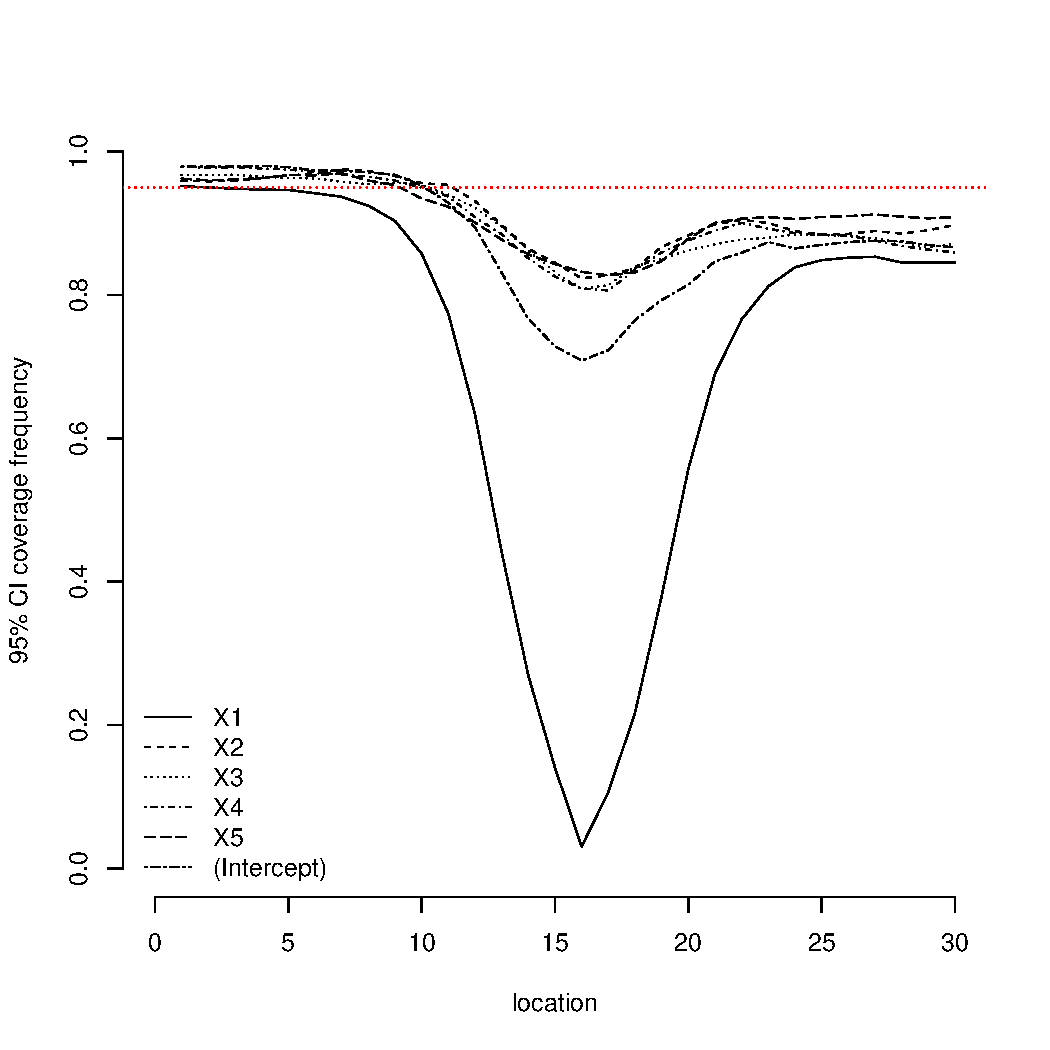
\includegraphics[width=\textwidth]{../../figures/simulation/15.1.profile_bootstrap_coverage.pdf}
		\caption{Bootstrap CI coverage}
		%\label{fig:gull}
	\end{subfigure}%
	~ %add desired spacing between images, e. g. ~, \quad, \qquad etc. 
	%(or a blank line to force the subfigure onto a new line)
	\begin{subfigure}[b]{0.45\textwidth}
	\centering
		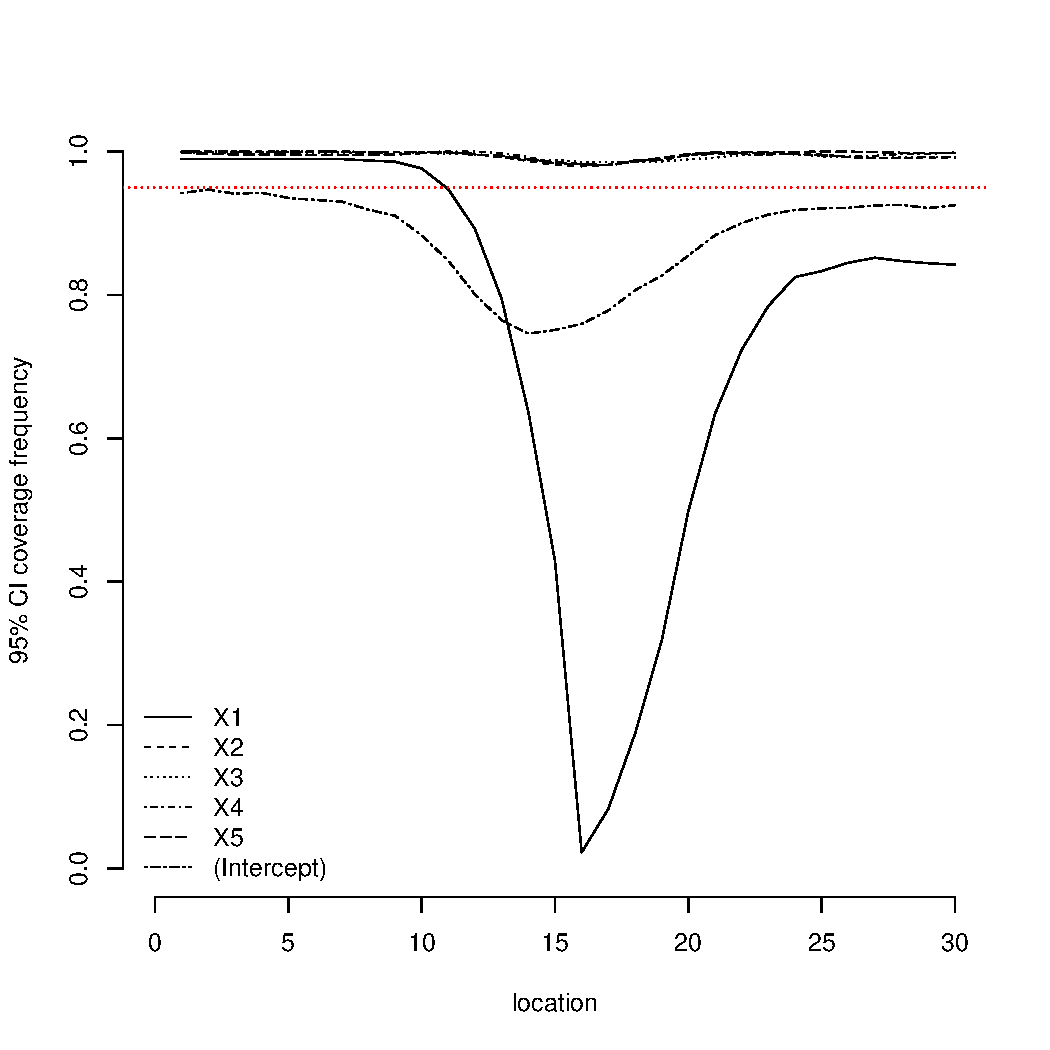
\includegraphics[width=\textwidth]{../../figures/simulation/15.1.profile_se_coverage.pdf}
		\caption{SE CI coverage}
		%\label{fig:gull}
	\end{subfigure}%
	\\%add desired spacing between images, e. g. ~, \quad, \qquad etc. 
          %(or a blank line to force the subfigure onto a new line)
	\begin{subfigure}[b]{0.45\textwidth}
	\centering
		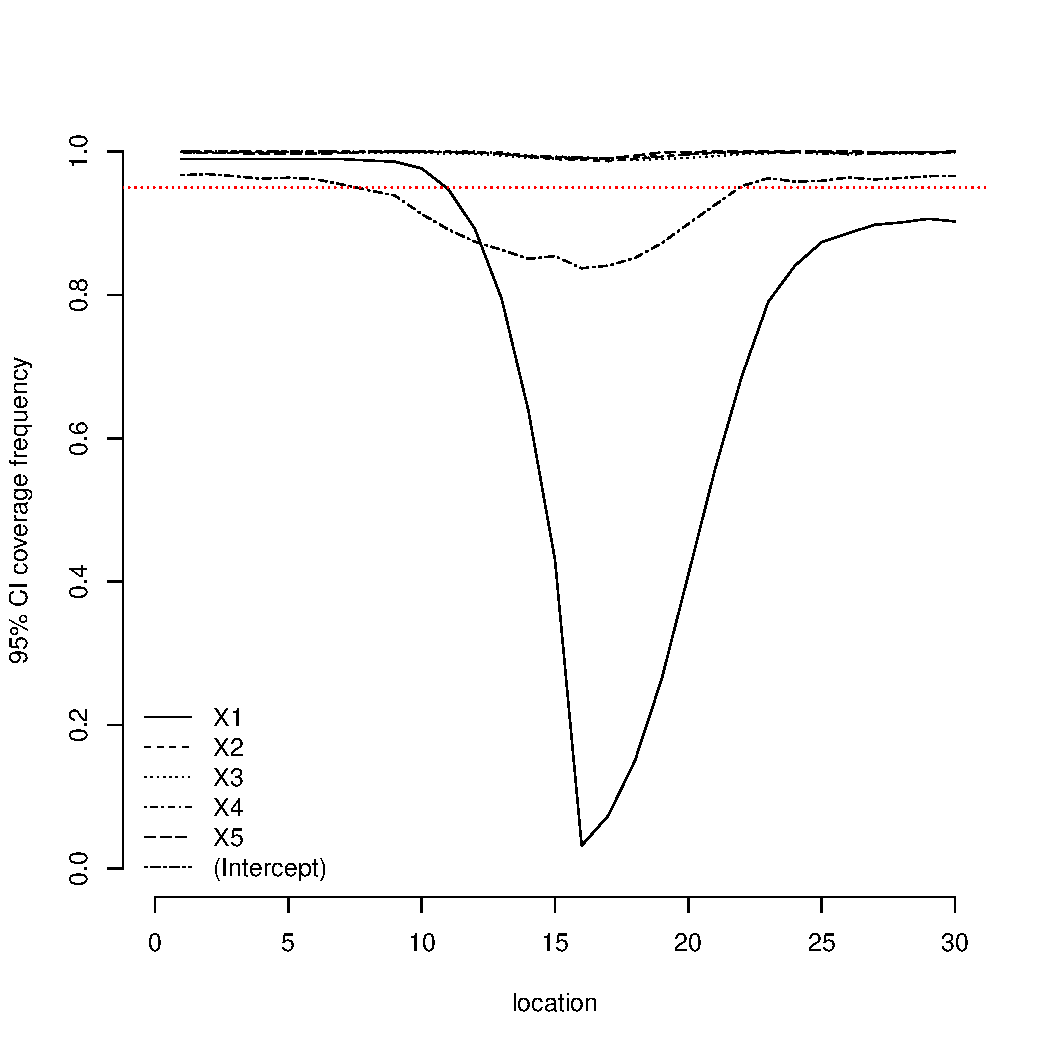
\includegraphics[width=\textwidth]{../../figures/simulation/15.1.profile_unshrunk_bootstrap_coverage.pdf}
		\caption{Unshrunk bootstrap CI coverage}
		%\label{fig:gull}
	\end{subfigure}%
	~ %add desired spacing between images, e. g. ~, \quad, \qquad etc. 
	%(or a blank line to force the subfigure onto a new line)
	\begin{subfigure}[b]{0.45\textwidth}
	\centering
		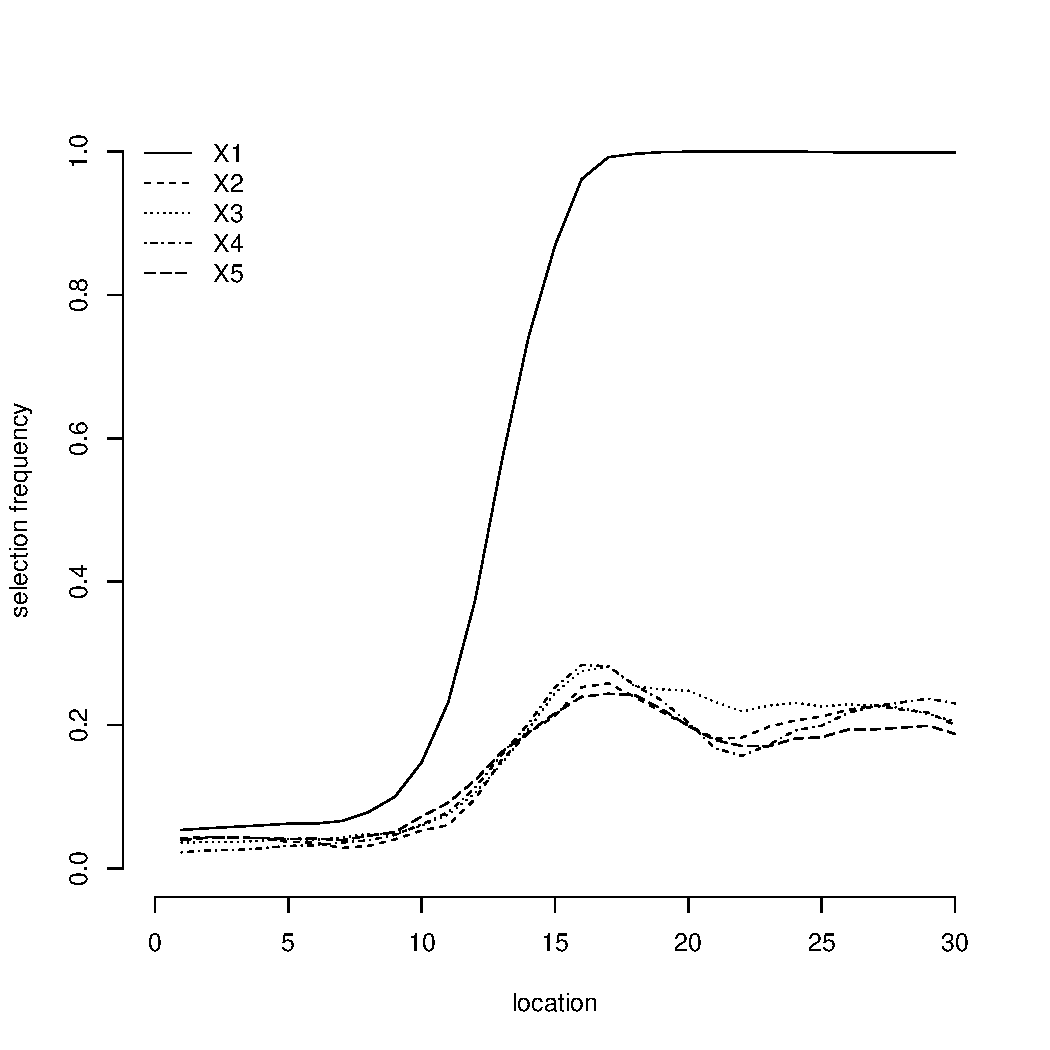
\includegraphics[width=\textwidth]{../../figures/simulation/15.1.profile_selection.pdf}
		\caption{Selection frequency}
		%\label{fig:gull}
	\end{subfigure}
	\begin{subfigure}[b]{0.45\textwidth}
	\centering
		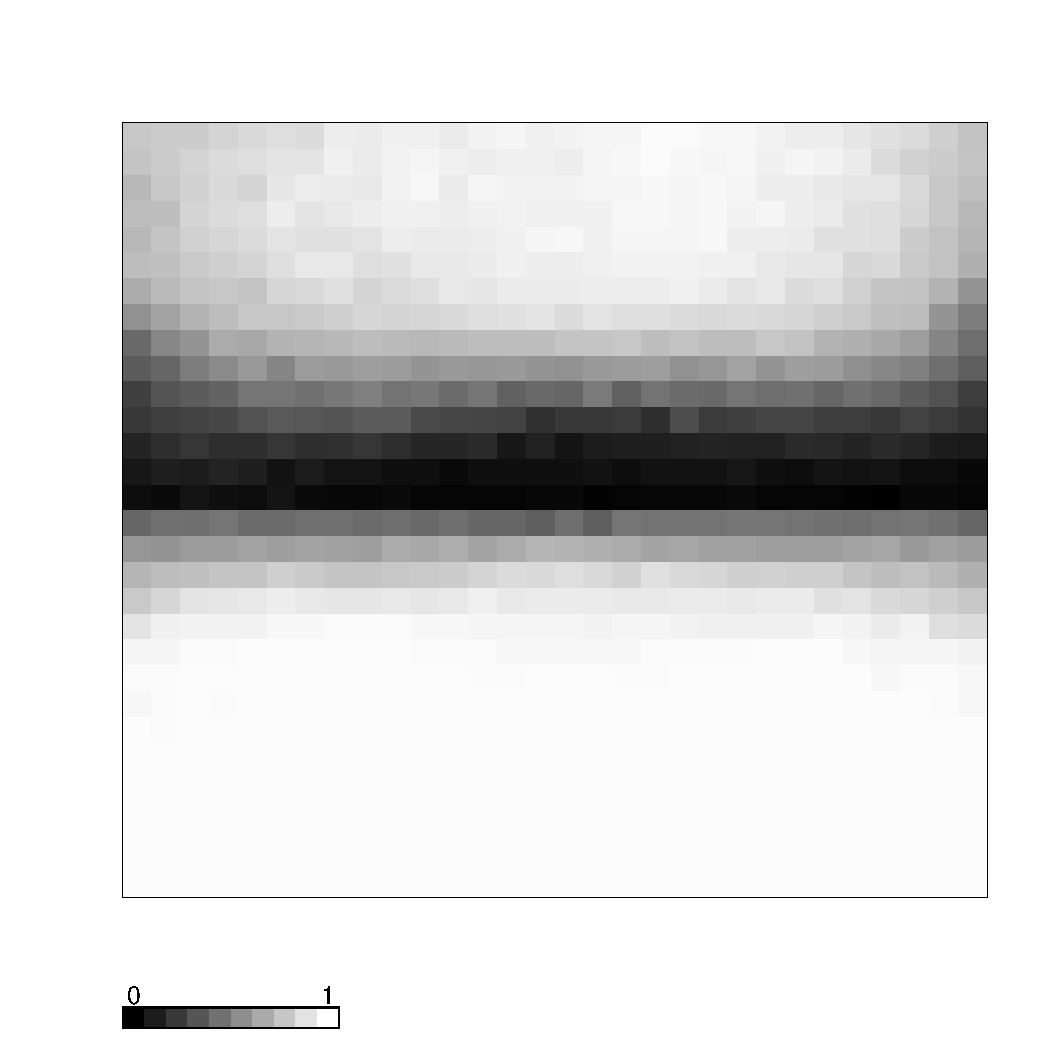
\includegraphics[width=\textwidth]{../../figures/simulation/X1.15.1.unshrunk_bootstrap_coverage.pdf}
		\caption{Unshrunk bootstrap CI coverage}
		%\label{fig:gull}
	\end{subfigure}%
	~ %add desired spacing between images, e. g. ~, \quad, \qquad etc. 
	%(or a blank line to force the subfigure onto a new line)
	\begin{subfigure}[b]{0.45\textwidth}
	\centering
		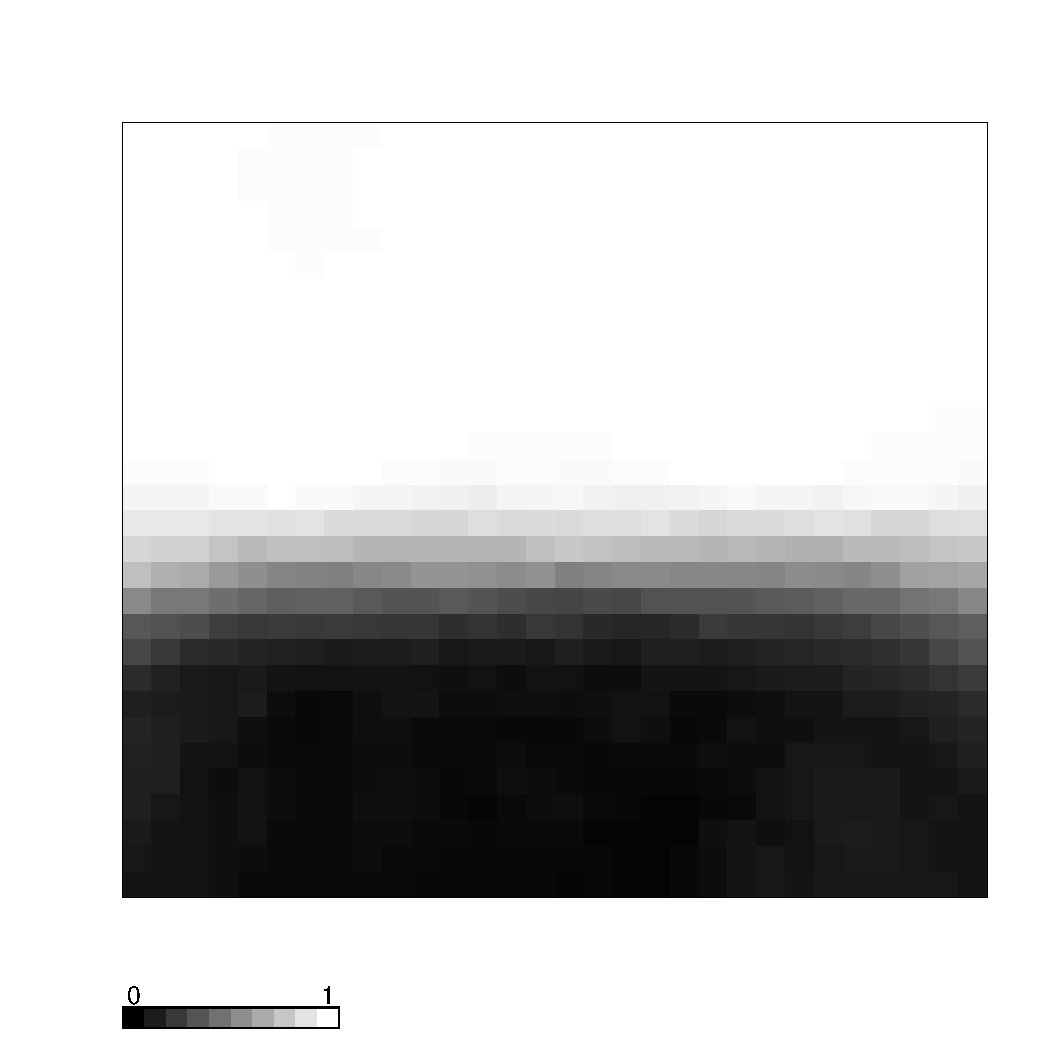
\includegraphics[width=\textwidth]{../../figures/simulation/X1.15.1.selection.pdf}
		\caption{Selection frequency}
		%\label{fig:gull}
	\end{subfigure}
	\caption{Simulation setting 1}
\end{figure}

\clearpage

\begin{figure}
	\vspace{-30mm}
	\centering
	\begin{subfigure}[b]{0.45\textwidth}
	\centering
		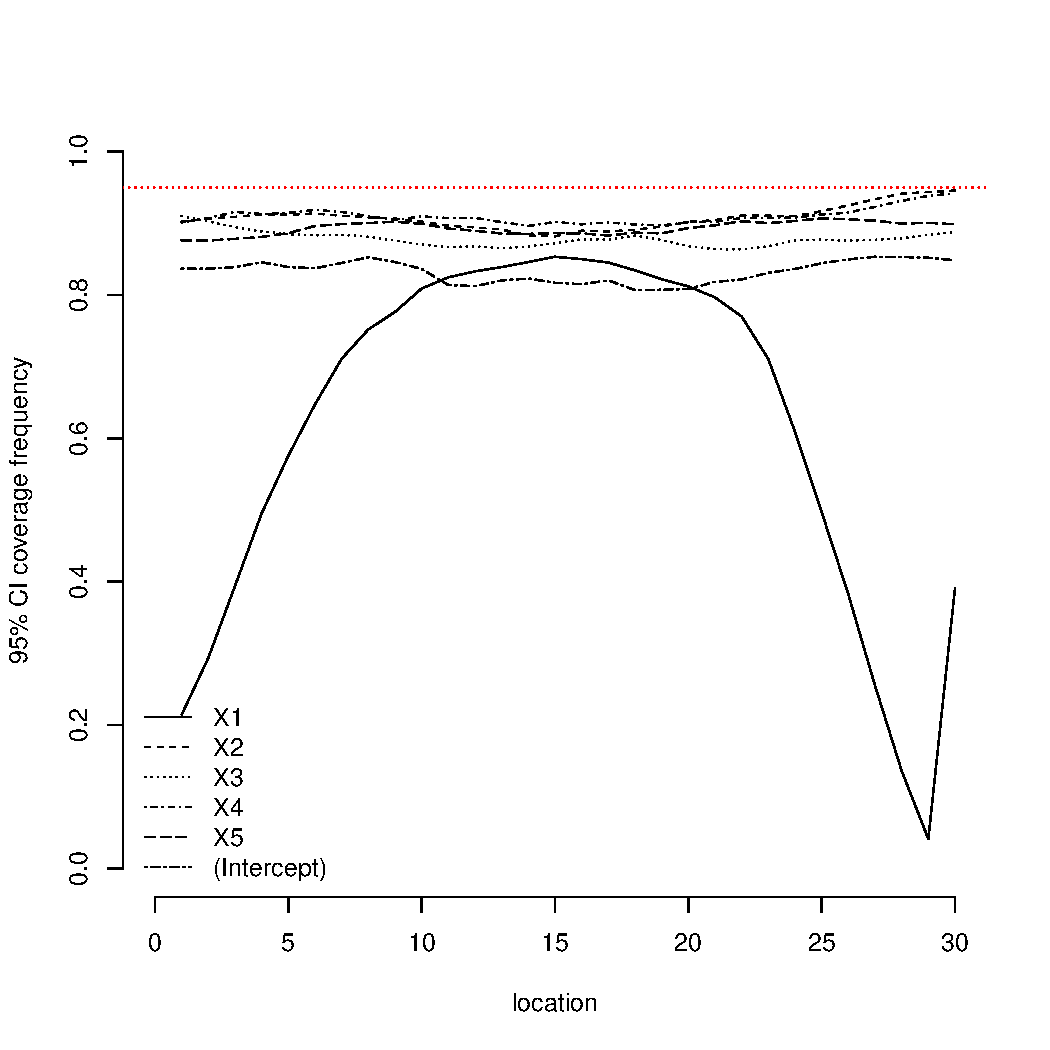
\includegraphics[width=\textwidth]{../../figures/simulation/15.2.profile_bootstrap_coverage.pdf}
		\caption{Bootstrap CI coverage}
		%\label{fig:gull}
	\end{subfigure}%
	~ %add desired spacing between images, e. g. ~, \quad, \qquad etc. 
	%(or a blank line to force the subfigure onto a new line)
	\begin{subfigure}[b]{0.45\textwidth}
	\centering
		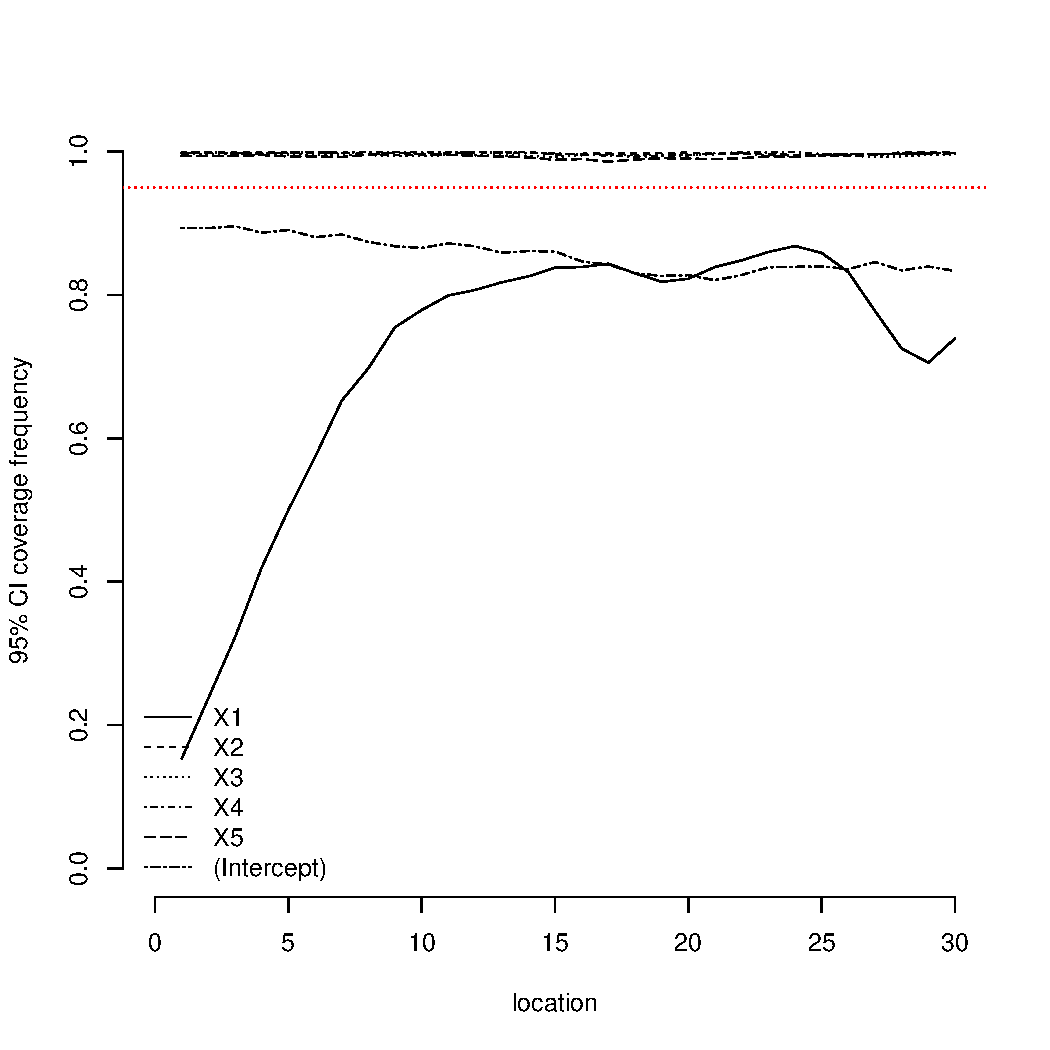
\includegraphics[width=\textwidth]{../../figures/simulation/15.2.profile_se_coverage.pdf}
		\caption{SE CI coverage}
		%\label{fig:gull}
	\end{subfigure}%
	\\%add desired spacing between images, e. g. ~, \quad, \qquad etc. 
          %(or a blank line to force the subfigure onto a new line)
	\begin{subfigure}[b]{0.45\textwidth}
	\centering
		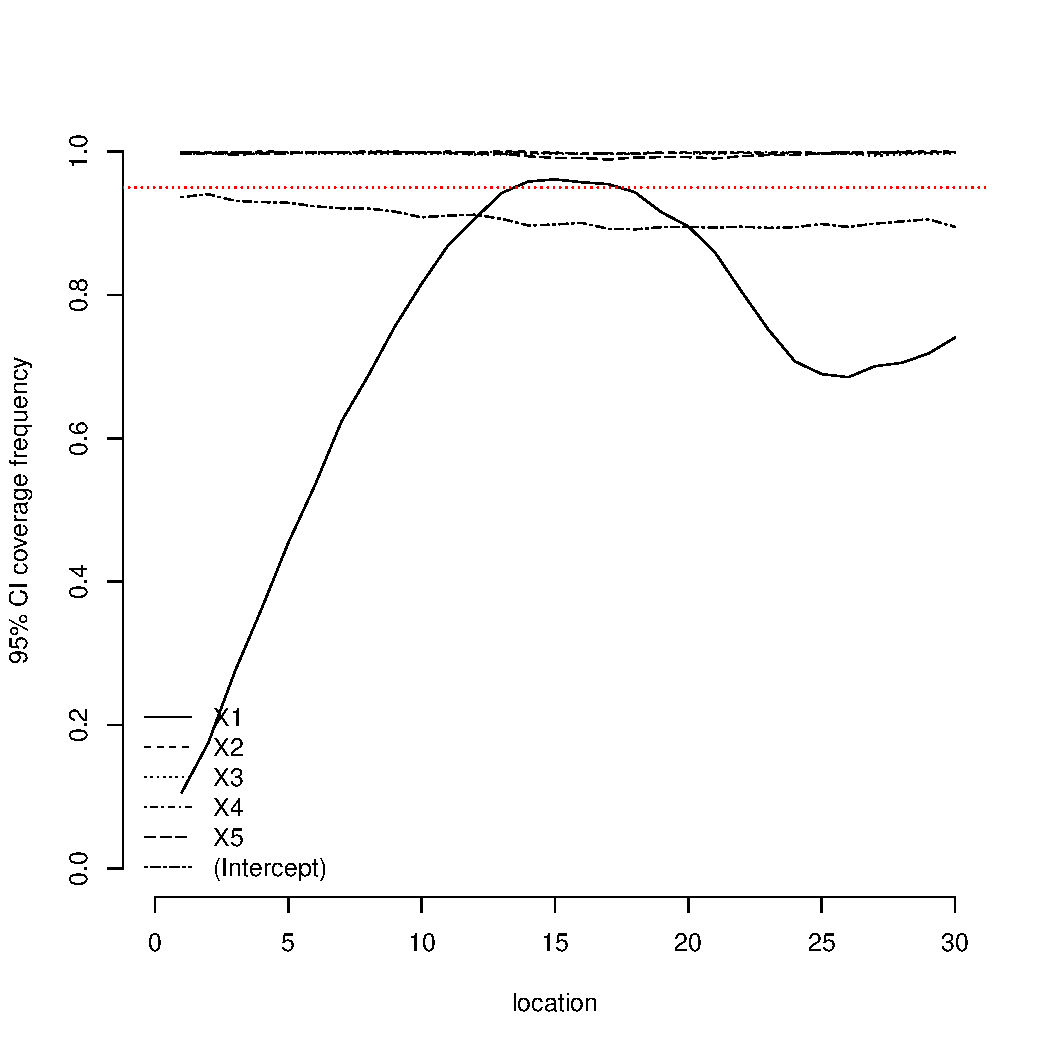
\includegraphics[width=\textwidth]{../../figures/simulation/15.2.profile_unshrunk_bootstrap_coverage.pdf}
		\caption{Unshrunk bootstrap CI coverage}
		%\label{fig:gull}
	\end{subfigure}%
	~ %add desired spacing between images, e. g. ~, \quad, \qquad etc. 
	%(or a blank line to force the subfigure onto a new line)
	\begin{subfigure}[b]{0.45\textwidth}
	\centering
		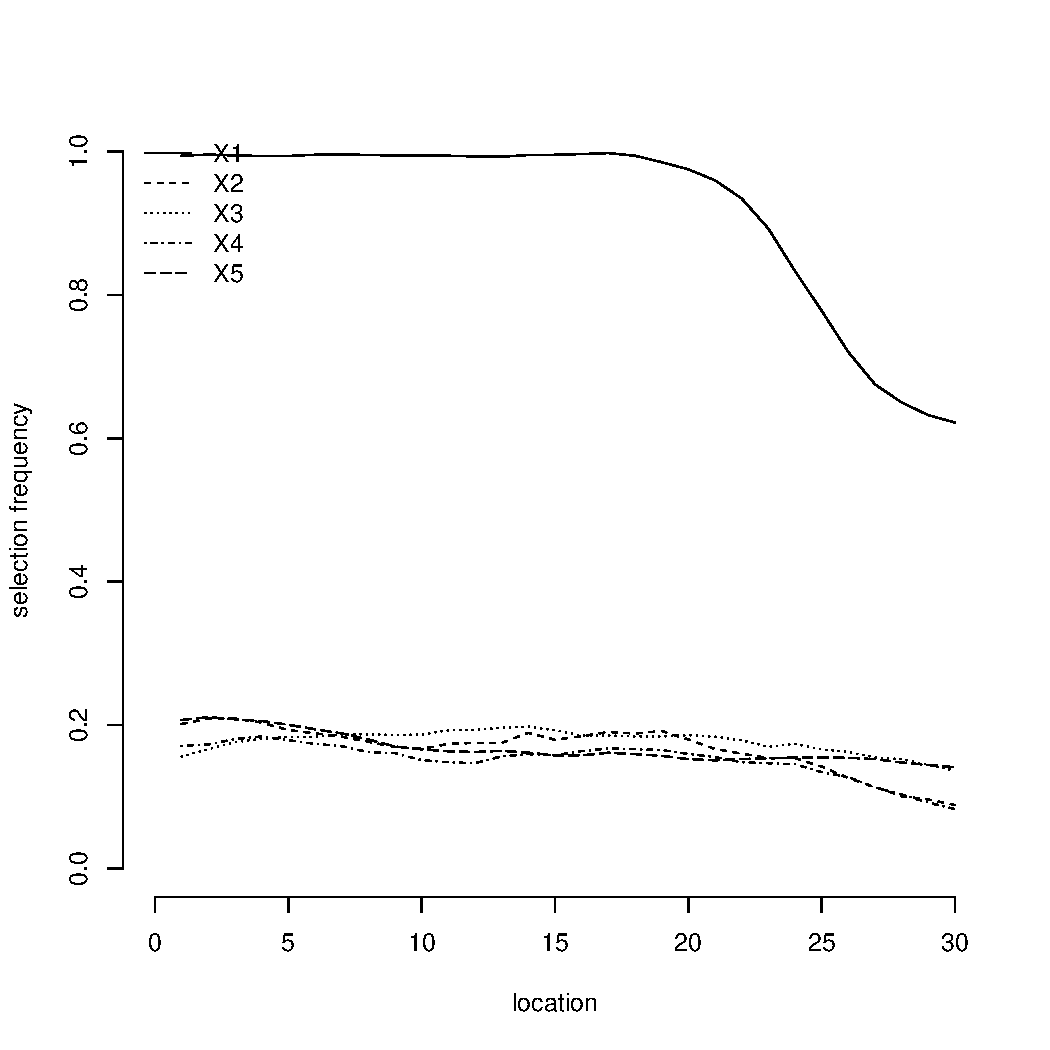
\includegraphics[width=\textwidth]{../../figures/simulation/15.2.profile_selection.pdf}
		\caption{Selection frequency}
		%\label{fig:gull}
	\end{subfigure}
	\begin{subfigure}[b]{0.45\textwidth}
	\centering
		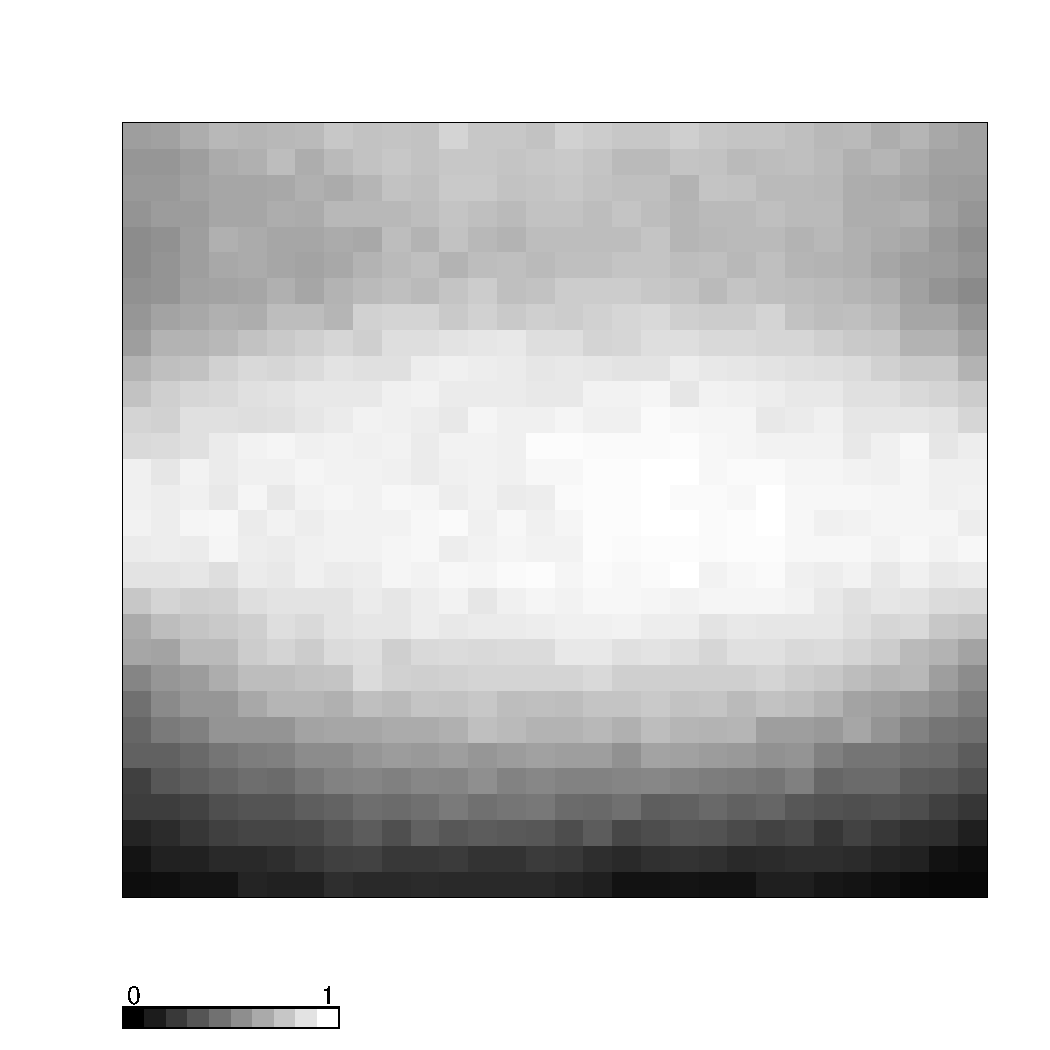
\includegraphics[width=\textwidth]{../../figures/simulation/X1.15.2.unshrunk_bootstrap_coverage.pdf}
		\caption{Unshrunk bootstrap CI coverage}
		%\label{fig:gull}
	\end{subfigure}%
	~ %add desired spacing between images, e. g. ~, \quad, \qquad etc. 
	%(or a blank line to force the subfigure onto a new line)
	\begin{subfigure}[b]{0.45\textwidth}
	\centering
		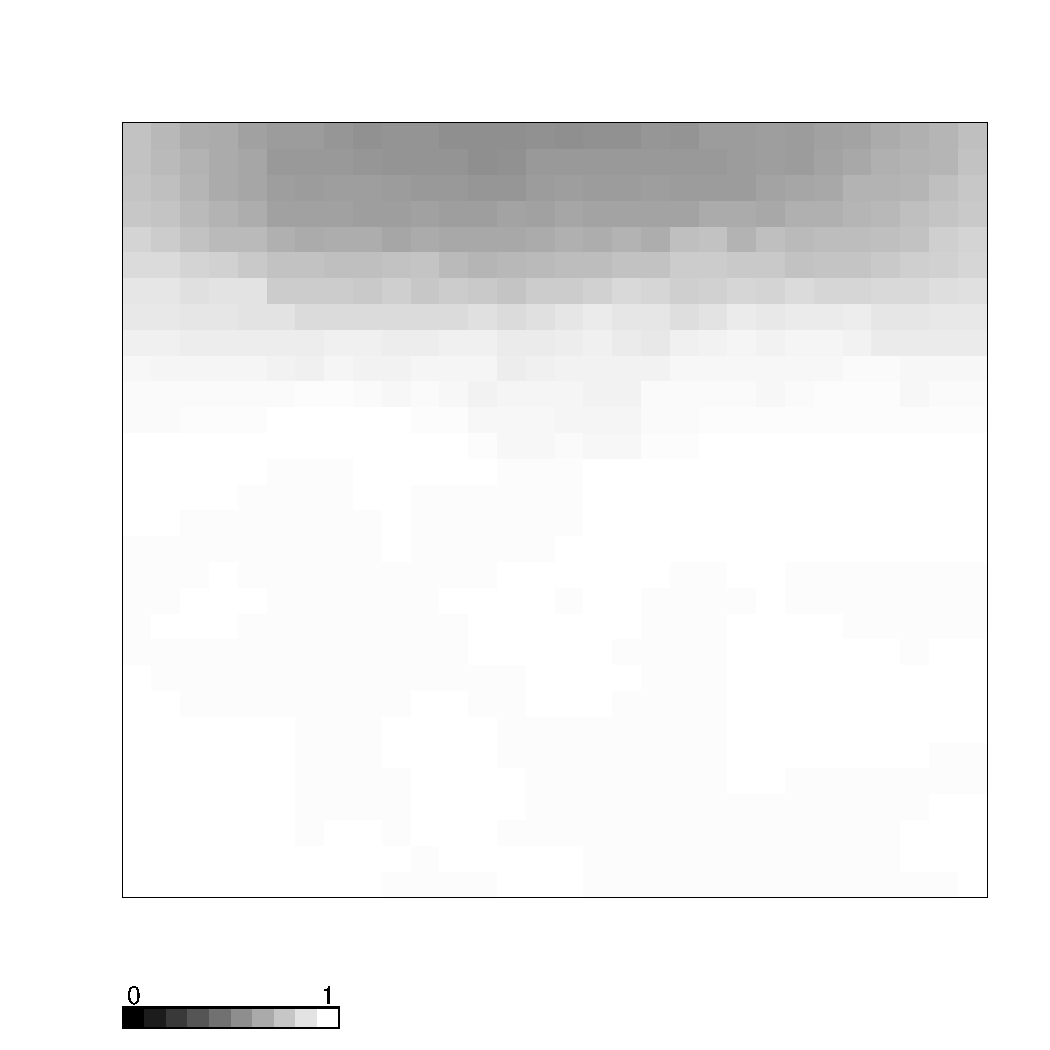
\includegraphics[width=\textwidth]{../../figures/simulation/X1.15.2.selection.pdf}
		\caption{Selection frequency}
		%\label{fig:gull}
	\end{subfigure}
	\caption{Simulation setting 2}
\end{figure}

\clearpage

\begin{figure}
	\vspace{-30mm}
	\centering
	\begin{subfigure}[b]{0.45\textwidth}
	\centering
		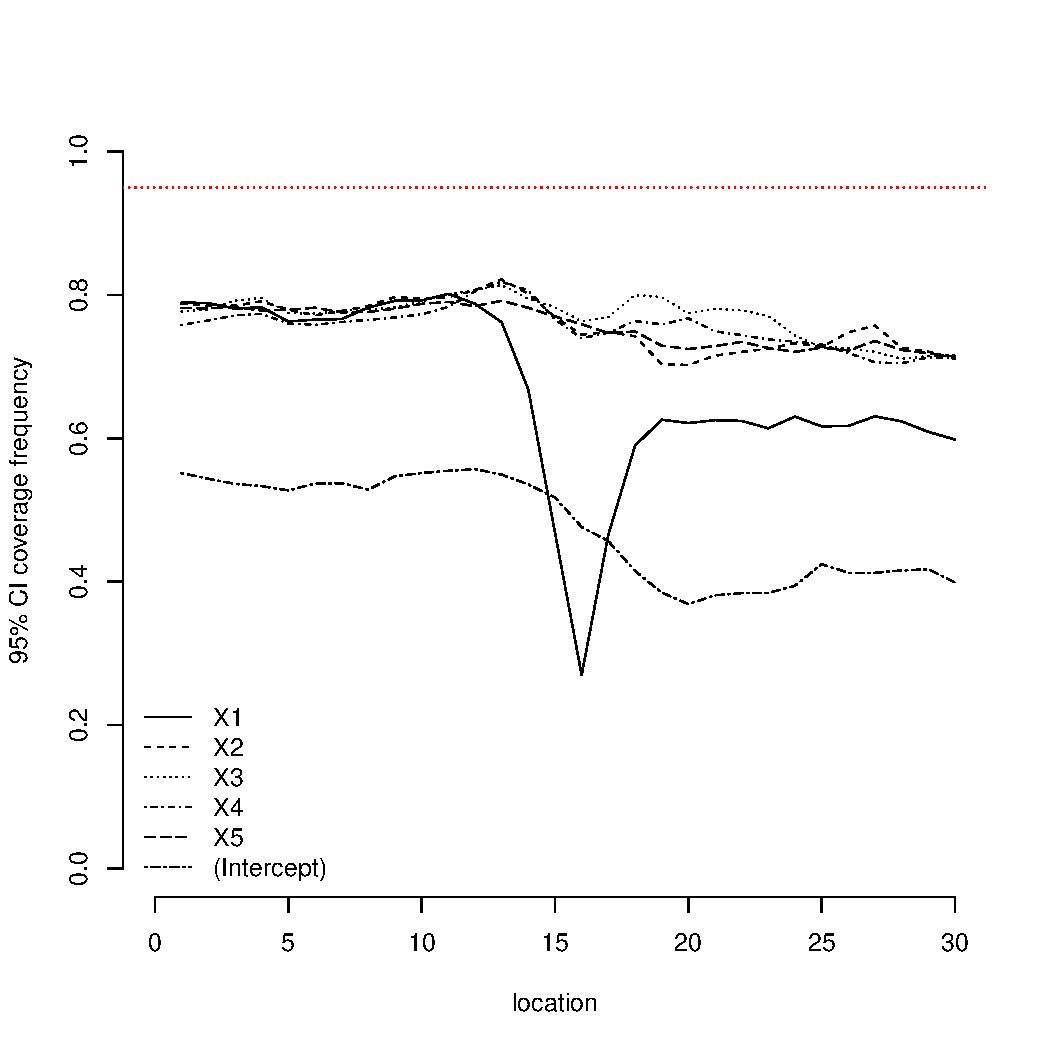
\includegraphics[width=\textwidth]{../../figures/simulation/15.3.profile_bootstrap_coverage.pdf}
		\caption{Bootstrap CI coverage}
		%\label{fig:gull}
	\end{subfigure}%
	~ %add desired spacing between images, e. g. ~, \quad, \qquad etc. 
	%(or a blank line to force the subfigure onto a new line)
	\begin{subfigure}[b]{0.45\textwidth}
	\centering
		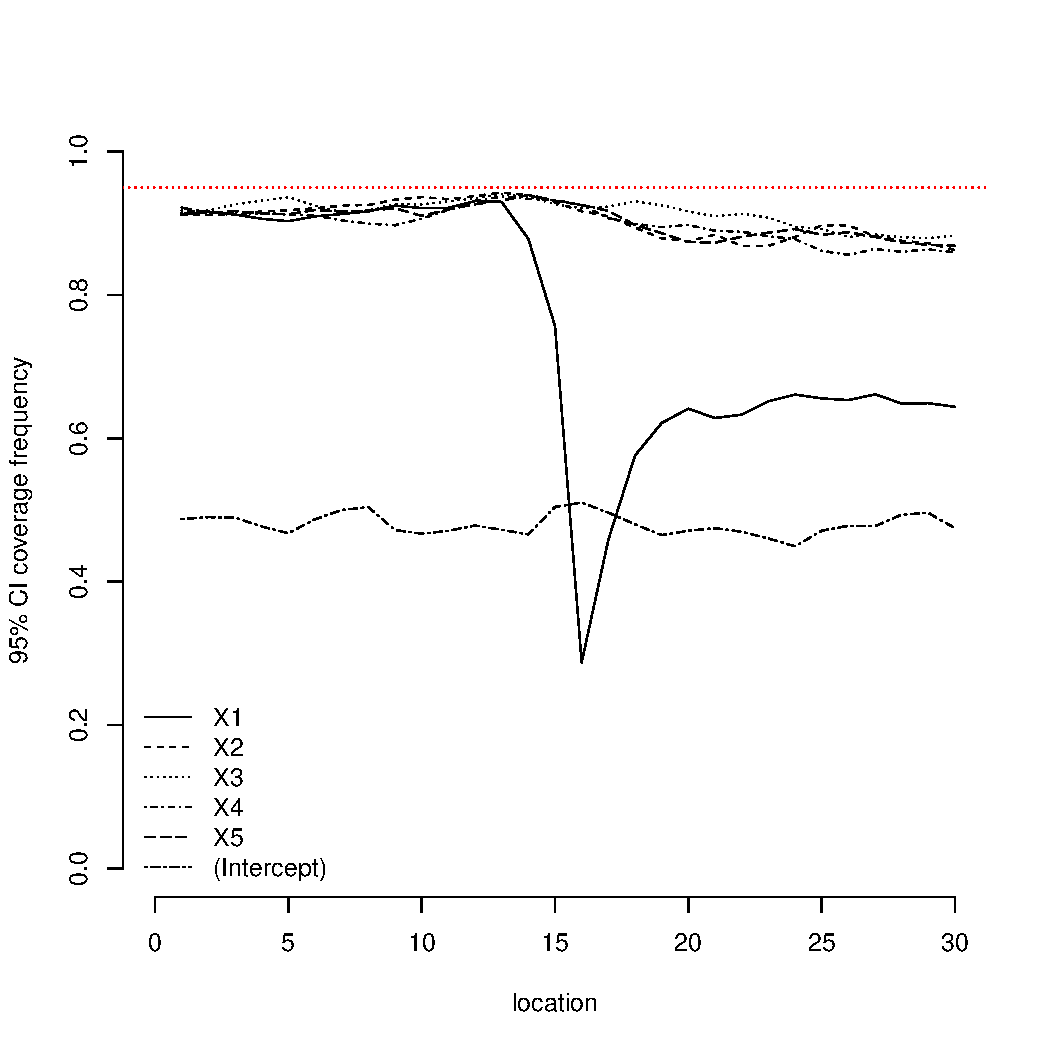
\includegraphics[width=\textwidth]{../../figures/simulation/15.3.profile_se_coverage.pdf}
		\caption{SE CI coverage}
		%\label{fig:gull}
	\end{subfigure}%
	\\%add desired spacing between images, e. g. ~, \quad, \qquad etc. 
          %(or a blank line to force the subfigure onto a new line)
	\begin{subfigure}[b]{0.45\textwidth}
	\centering
		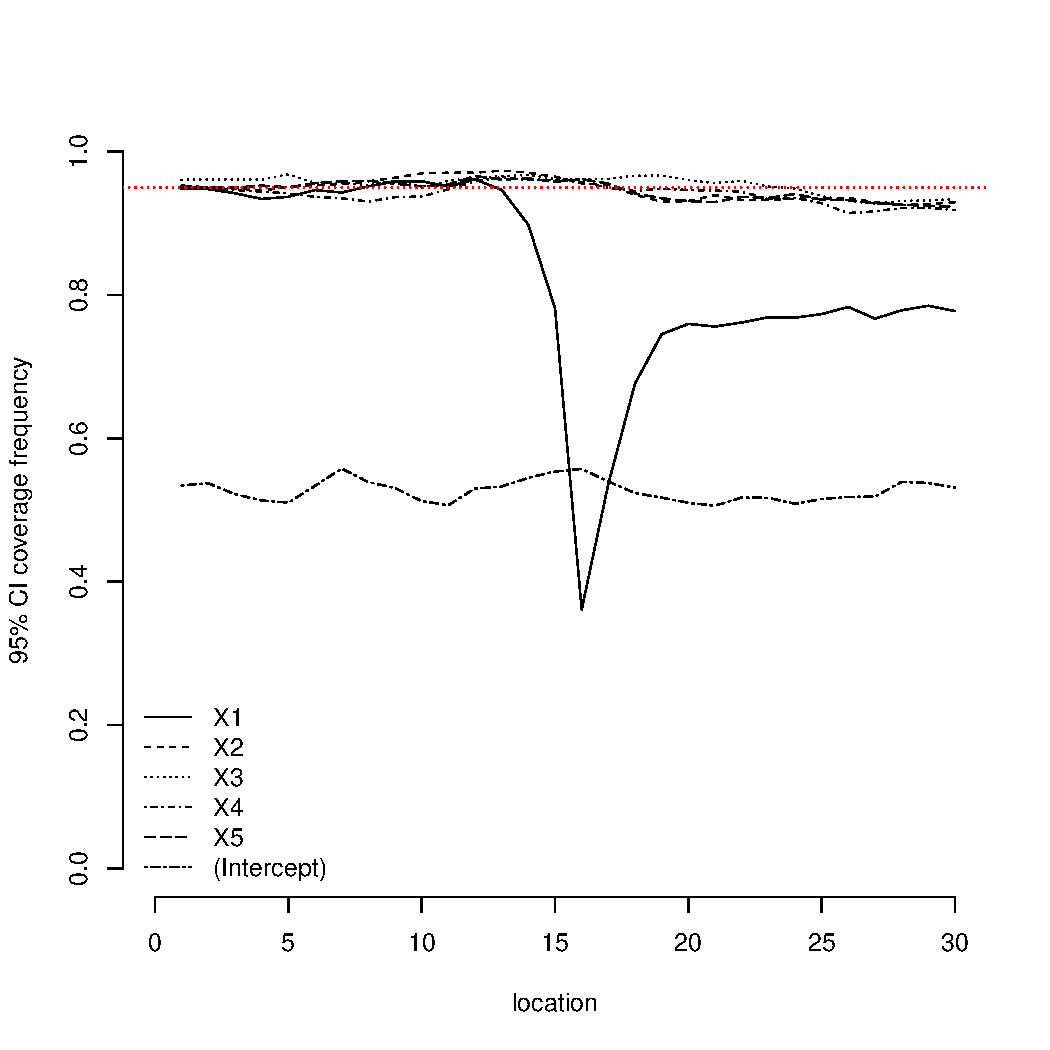
\includegraphics[width=\textwidth]{../../figures/simulation/15.3.profile_unshrunk_bootstrap_coverage.pdf}
		\caption{Unshrunk bootstrap CI coverage}
		%\label{fig:gull}
	\end{subfigure}%
	~ %add desired spacing between images, e. g. ~, \quad, \qquad etc. 
	%(or a blank line to force the subfigure onto a new line)
	\begin{subfigure}[b]{0.45\textwidth}
	\centering
		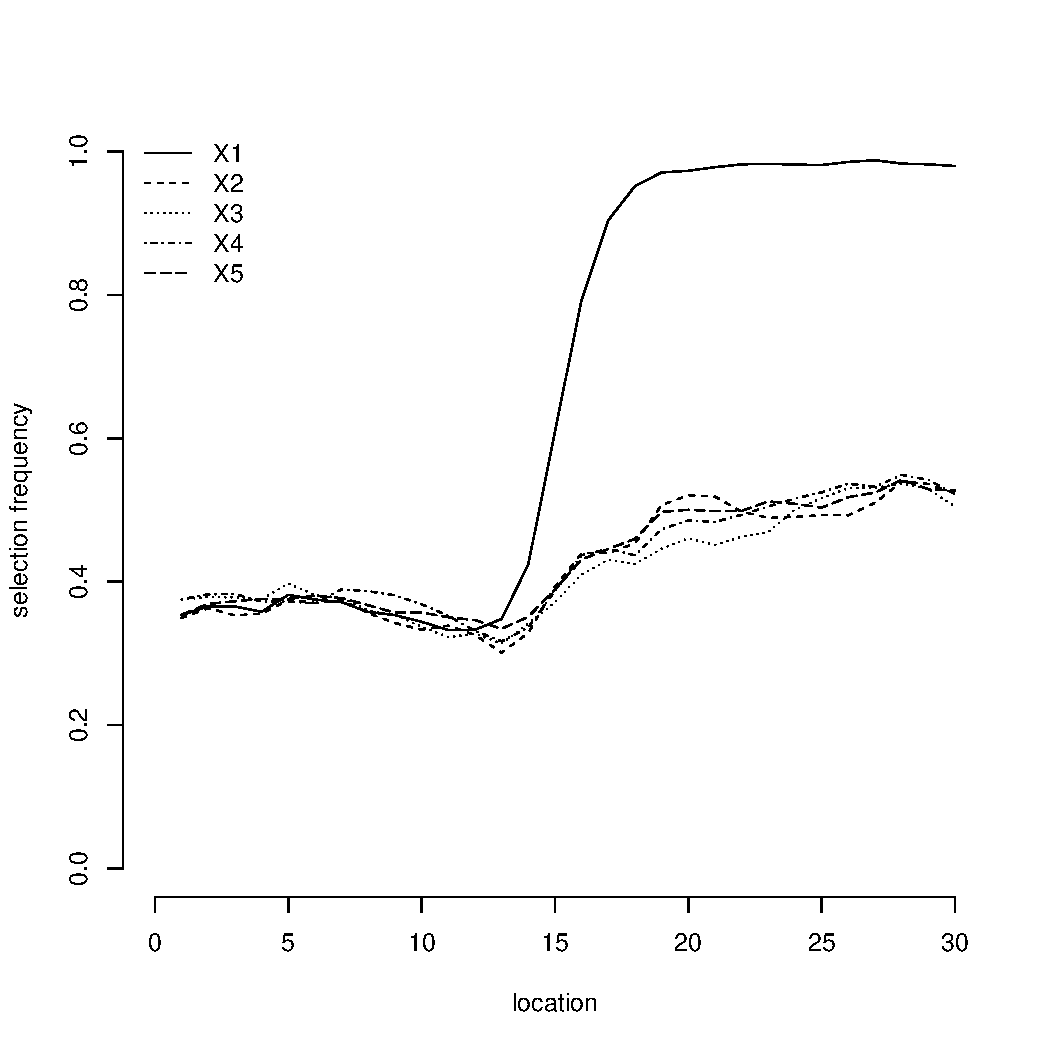
\includegraphics[width=\textwidth]{../../figures/simulation/15.3.profile_selection.pdf}
		\caption{Selection frequency}
		%\label{fig:gull}
	\end{subfigure}
	\begin{subfigure}[b]{0.45\textwidth}
	\centering
		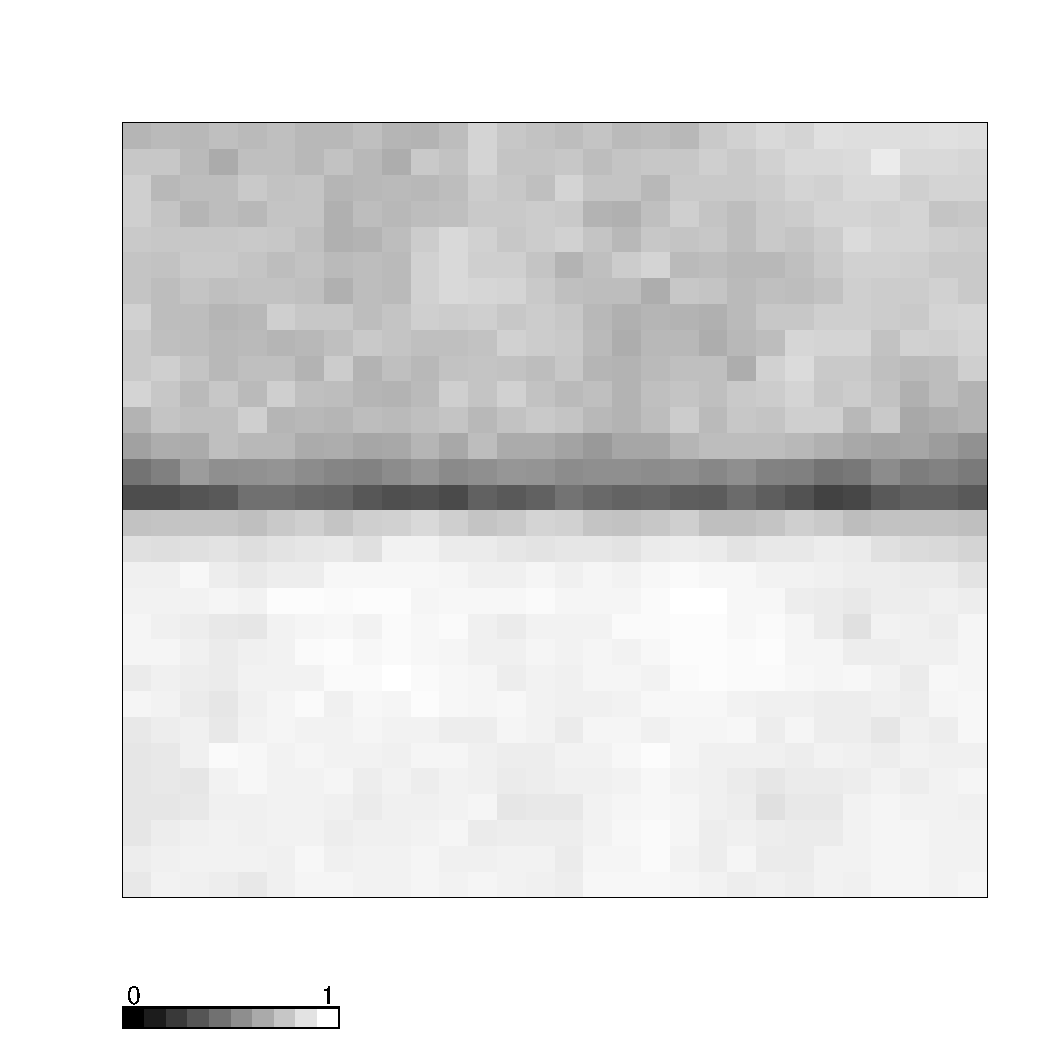
\includegraphics[width=\textwidth]{../../figures/simulation/X1.15.3.unshrunk_bootstrap_coverage.pdf}
		\caption{Unshrunk bootstrap CI coverage}
		%\label{fig:gull}
	\end{subfigure}%
	~ %add desired spacing between images, e. g. ~, \quad, \qquad etc. 
	%(or a blank line to force the subfigure onto a new line)
	\begin{subfigure}[b]{0.45\textwidth}
	\centering
		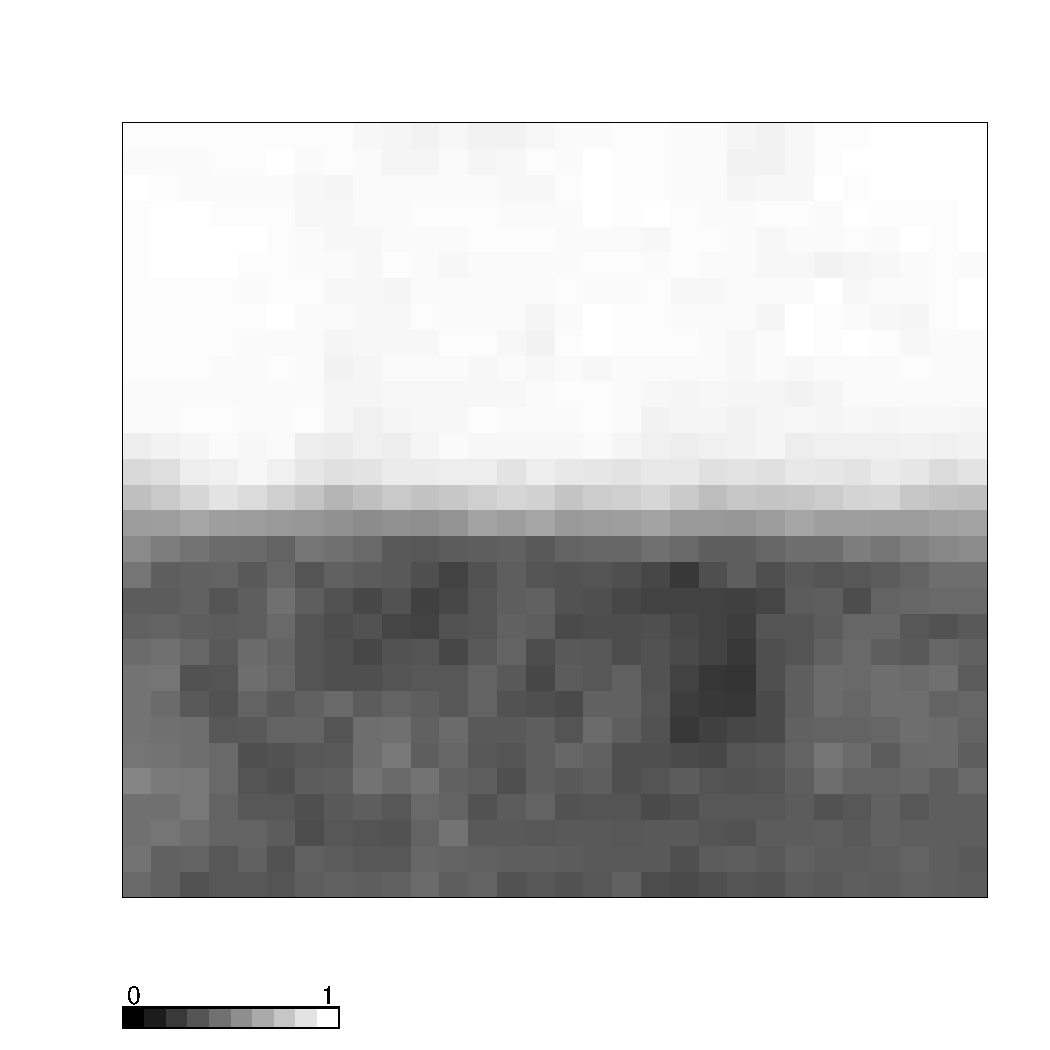
\includegraphics[width=\textwidth]{../../figures/simulation/X1.15.3.selection.pdf}
		\caption{Selection frequency}
		%\label{fig:gull}
	\end{subfigure}
	\caption{Simulation setting 3}
\end{figure}

\clearpage

\begin{figure}
	\vspace{-30mm}
	\centering
	\begin{subfigure}[b]{0.45\textwidth}
	\centering
		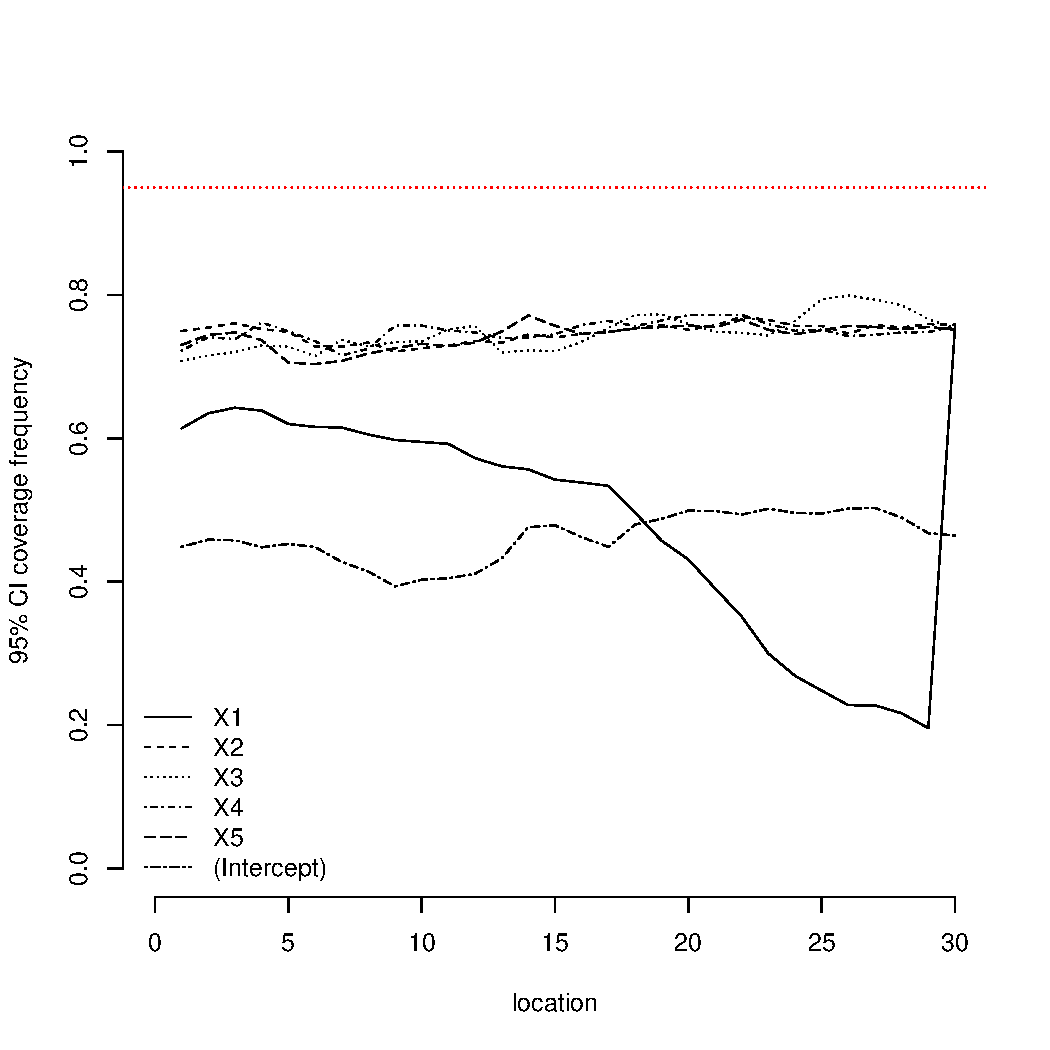
\includegraphics[width=\textwidth]{../../figures/simulation/15.4.profile_bootstrap_coverage.pdf}
		\caption{Bootstrap CI coverage}
		%\label{fig:gull}
	\end{subfigure}%
	~ %add desired spacing between images, e. g. ~, \quad, \qquad etc. 
	%(or a blank line to force the subfigure onto a new line)
	\begin{subfigure}[b]{0.45\textwidth}
	\centering
		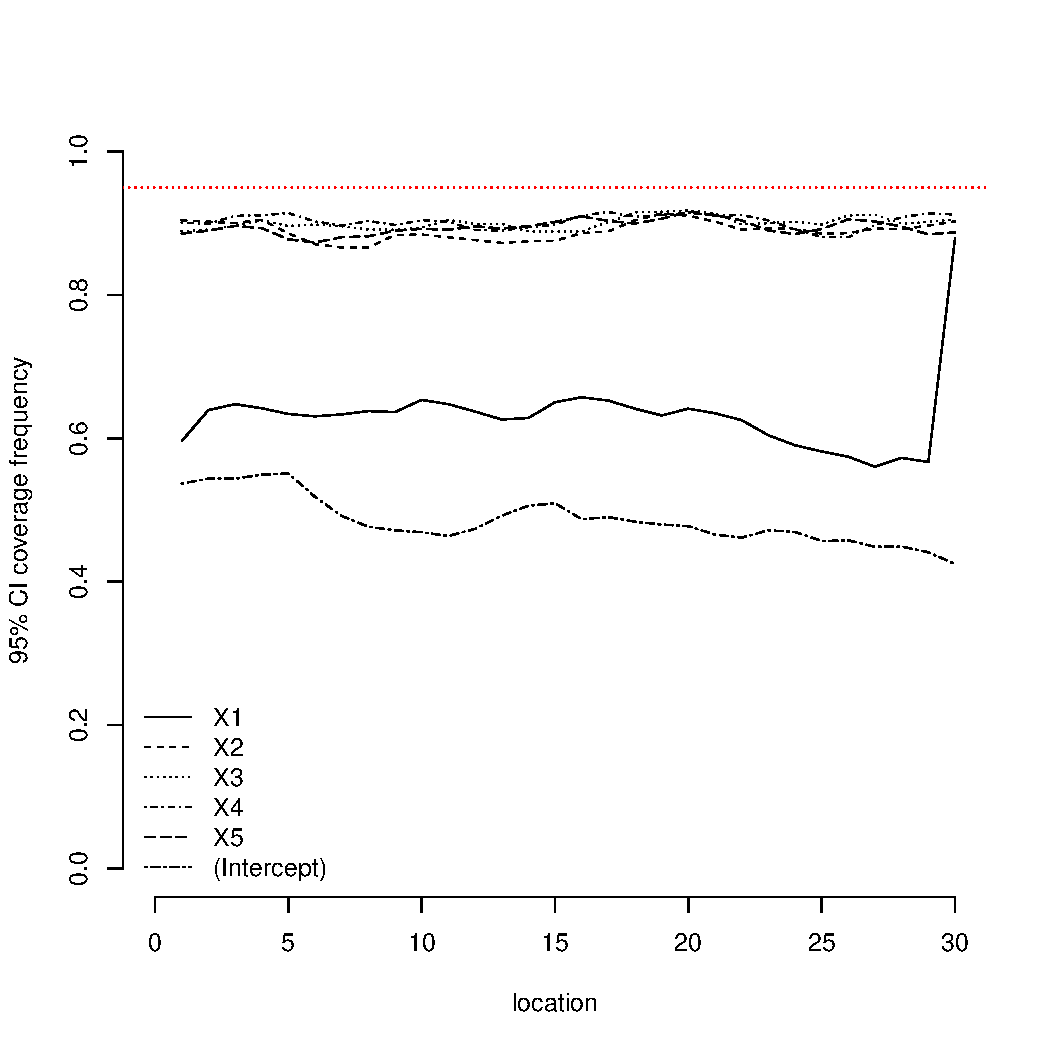
\includegraphics[width=\textwidth]{../../figures/simulation/15.4.profile_se_coverage.pdf}
		\caption{SE CI coverage}
		%\label{fig:gull}
	\end{subfigure}%
	\\%add desired spacing between images, e. g. ~, \quad, \qquad etc. 
          %(or a blank line to force the subfigure onto a new line)
	\begin{subfigure}[b]{0.45\textwidth}
	\centering
		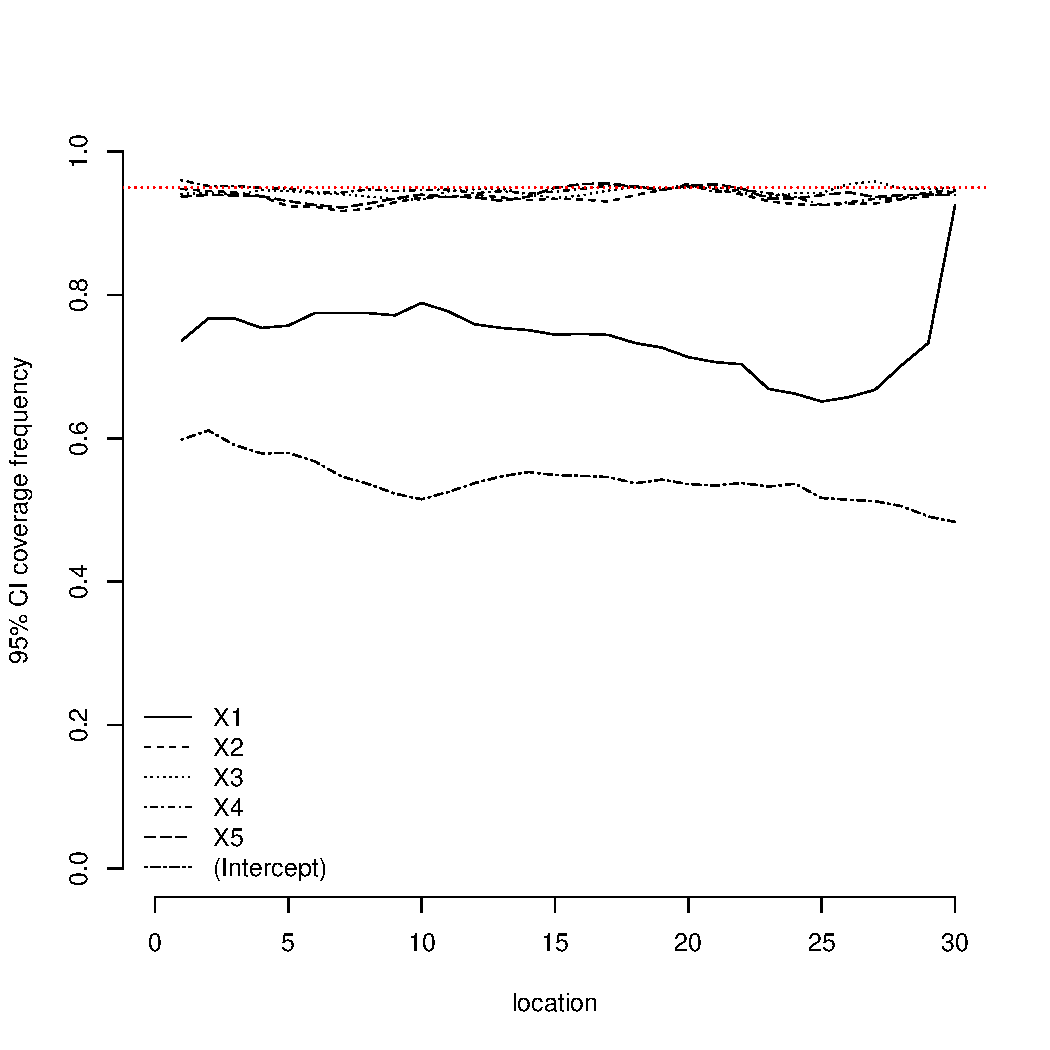
\includegraphics[width=\textwidth]{../../figures/simulation/15.4.profile_unshrunk_bootstrap_coverage.pdf}
		\caption{Unshrunk bootstrap CI coverage}
		%\label{fig:gull}
	\end{subfigure}%
	~ %add desired spacing between images, e. g. ~, \quad, \qquad etc. 
	%(or a blank line to force the subfigure onto a new line)
	\begin{subfigure}[b]{0.45\textwidth}
	\centering
		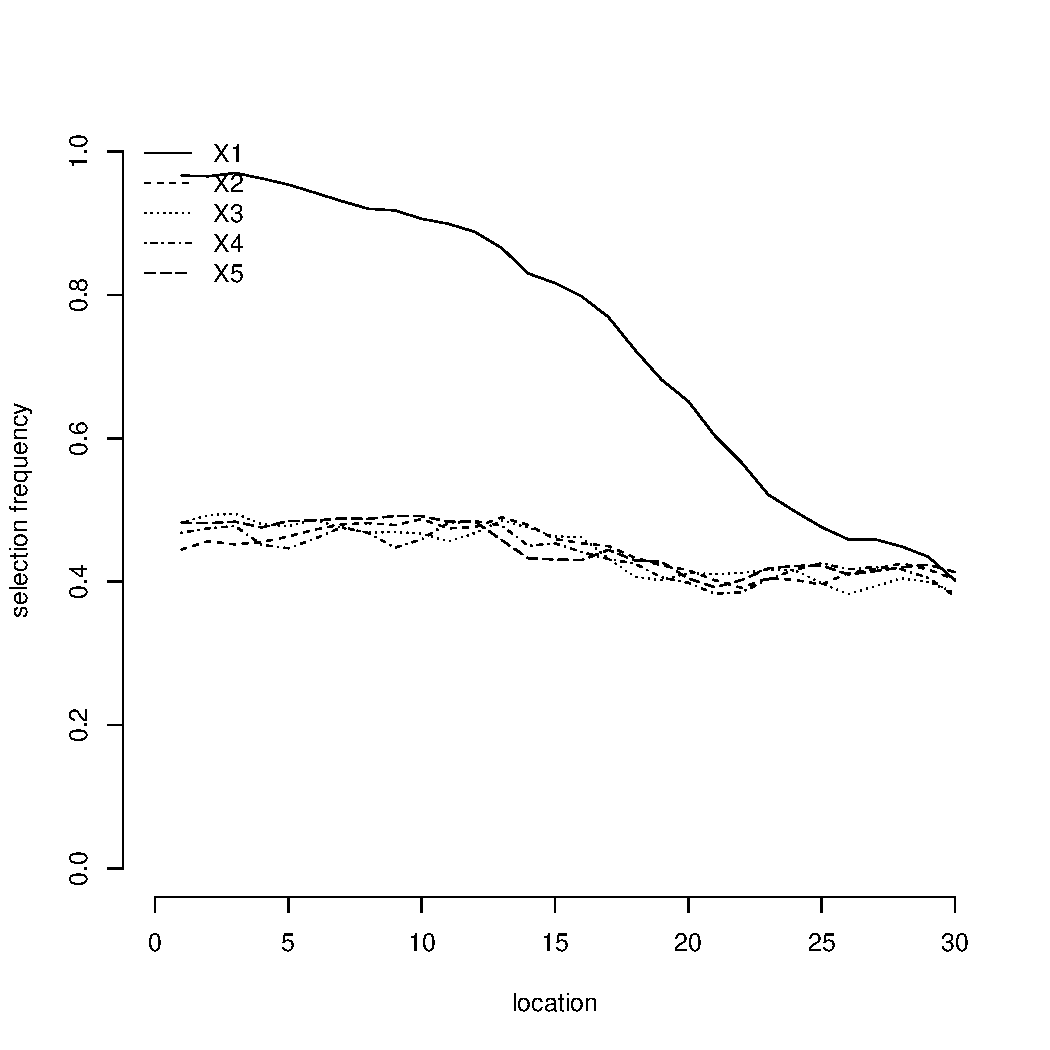
\includegraphics[width=\textwidth]{../../figures/simulation/15.4.profile_selection.pdf}
		\caption{Selection frequency}
		%\label{fig:gull}
	\end{subfigure}
	\begin{subfigure}[b]{0.45\textwidth}
	\centering
		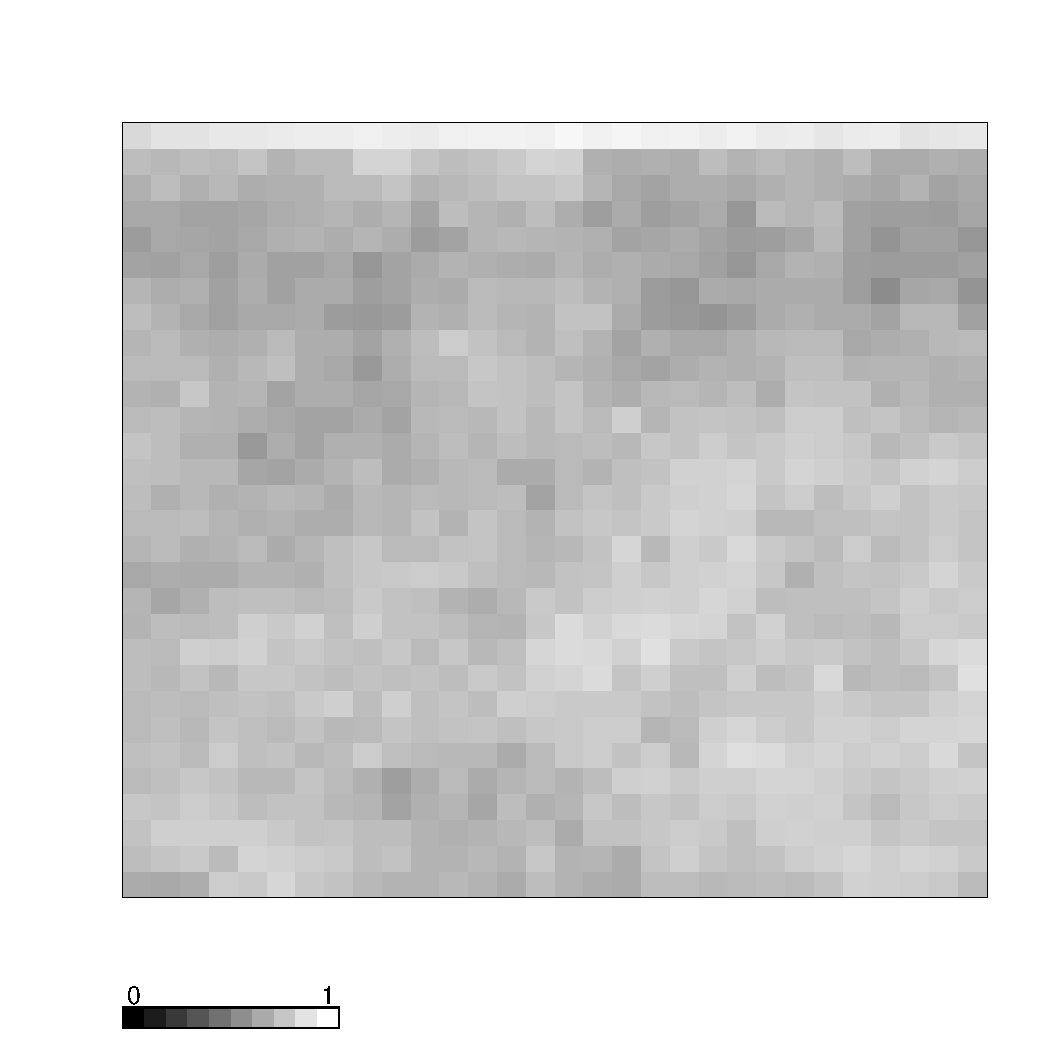
\includegraphics[width=\textwidth]{../../figures/simulation/X1.15.4.unshrunk_bootstrap_coverage.pdf}
		\caption{Unshrunk bootstrap CI coverage}
		%\label{fig:gull}
	\end{subfigure}%
	~ %add desired spacing between images, e. g. ~, \quad, \qquad etc. 
	%(or a blank line to force the subfigure onto a new line)
	\begin{subfigure}[b]{0.45\textwidth}
	\centering
		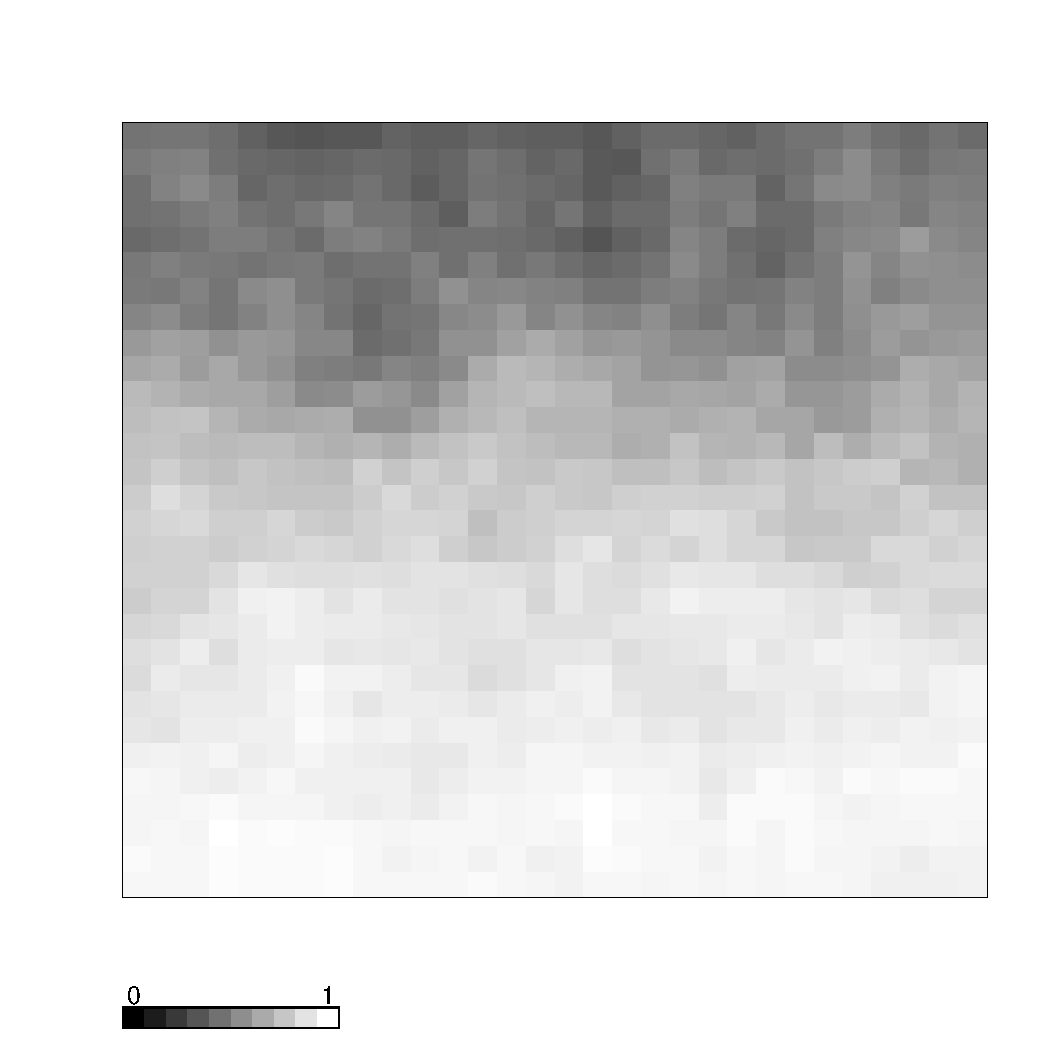
\includegraphics[width=\textwidth]{../../figures/simulation/X1.15.4.selection.pdf}
		\caption{Selection frequency}
		%\label{fig:gull}
	\end{subfigure}
	\caption{Simulation setting 4}
\end{figure}

\clearpage

\begin{figure}
	\vspace{-30mm}
	\centering
	\begin{subfigure}[b]{0.45\textwidth}
	\centering
		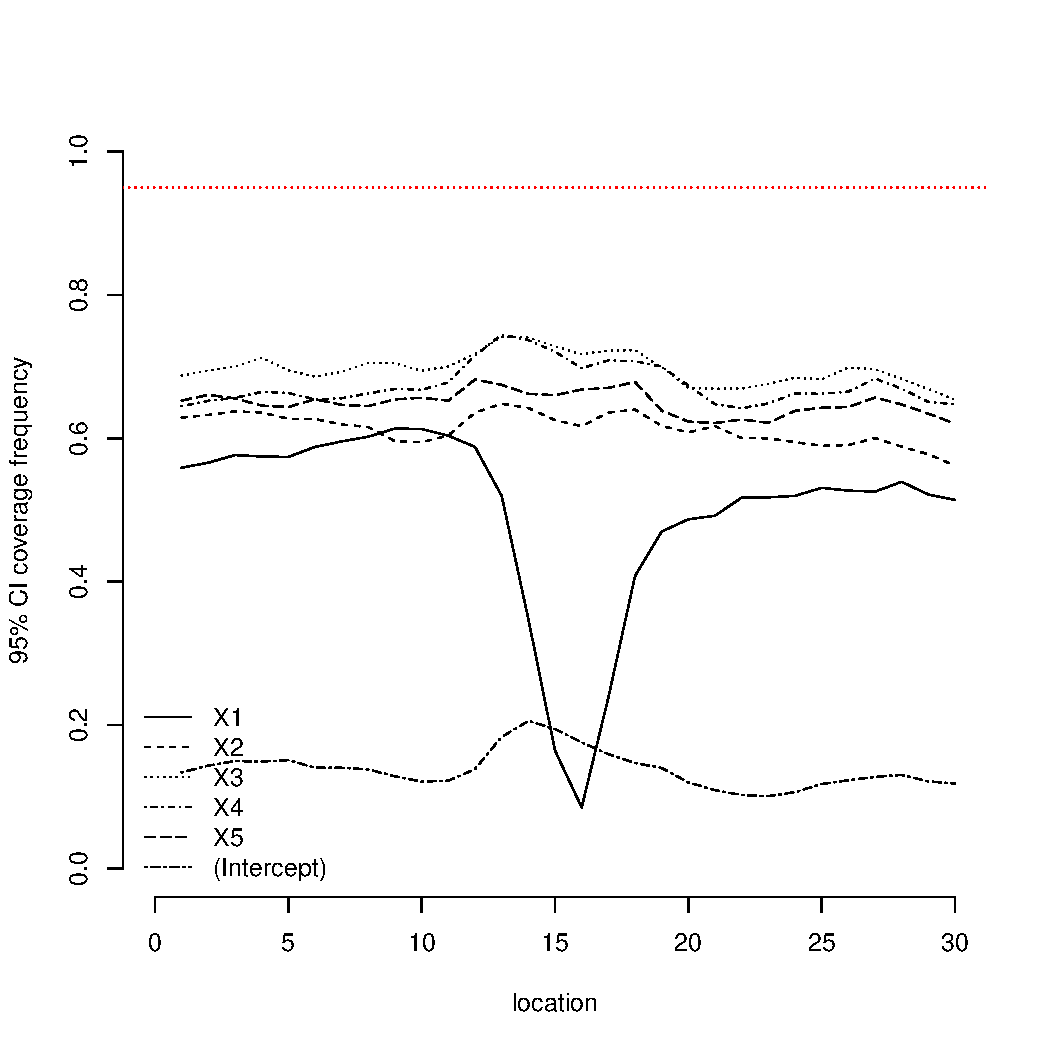
\includegraphics[width=\textwidth]{../../figures/simulation/15.5.profile_bootstrap_coverage.pdf}
		\caption{Bootstrap CI coverage}
		%\label{fig:gull}
	\end{subfigure}%
	~ %add desired spacing between images, e. g. ~, \quad, \qquad etc. 
	%(or a blank line to force the subfigure onto a new line)
	\begin{subfigure}[b]{0.45\textwidth}
	\centering
		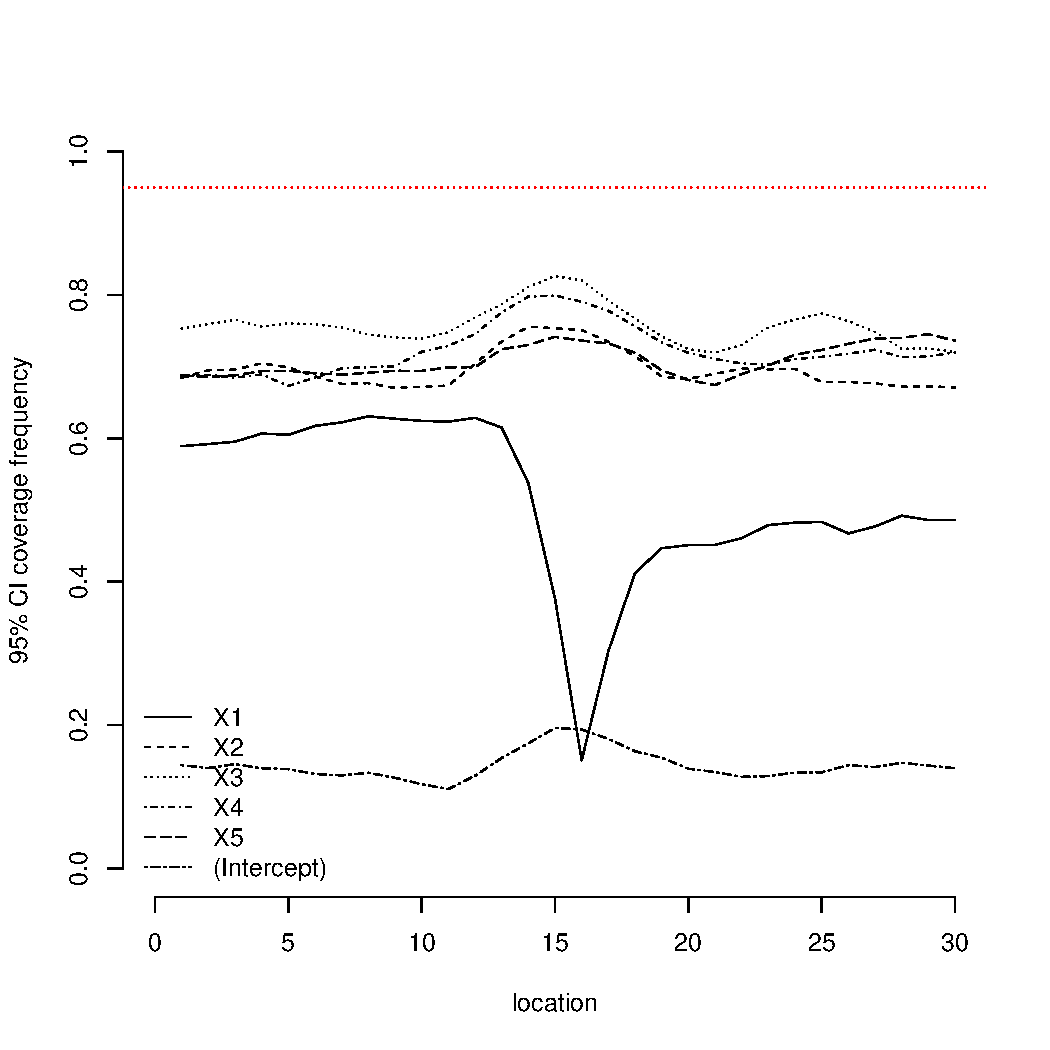
\includegraphics[width=\textwidth]{../../figures/simulation/15.5.profile_se_coverage.pdf}
		\caption{SE CI coverage}
		%\label{fig:gull}
	\end{subfigure}%
	\\%add desired spacing between images, e. g. ~, \quad, \qquad etc. 
          %(or a blank line to force the subfigure onto a new line)
	\begin{subfigure}[b]{0.45\textwidth}
	\centering
		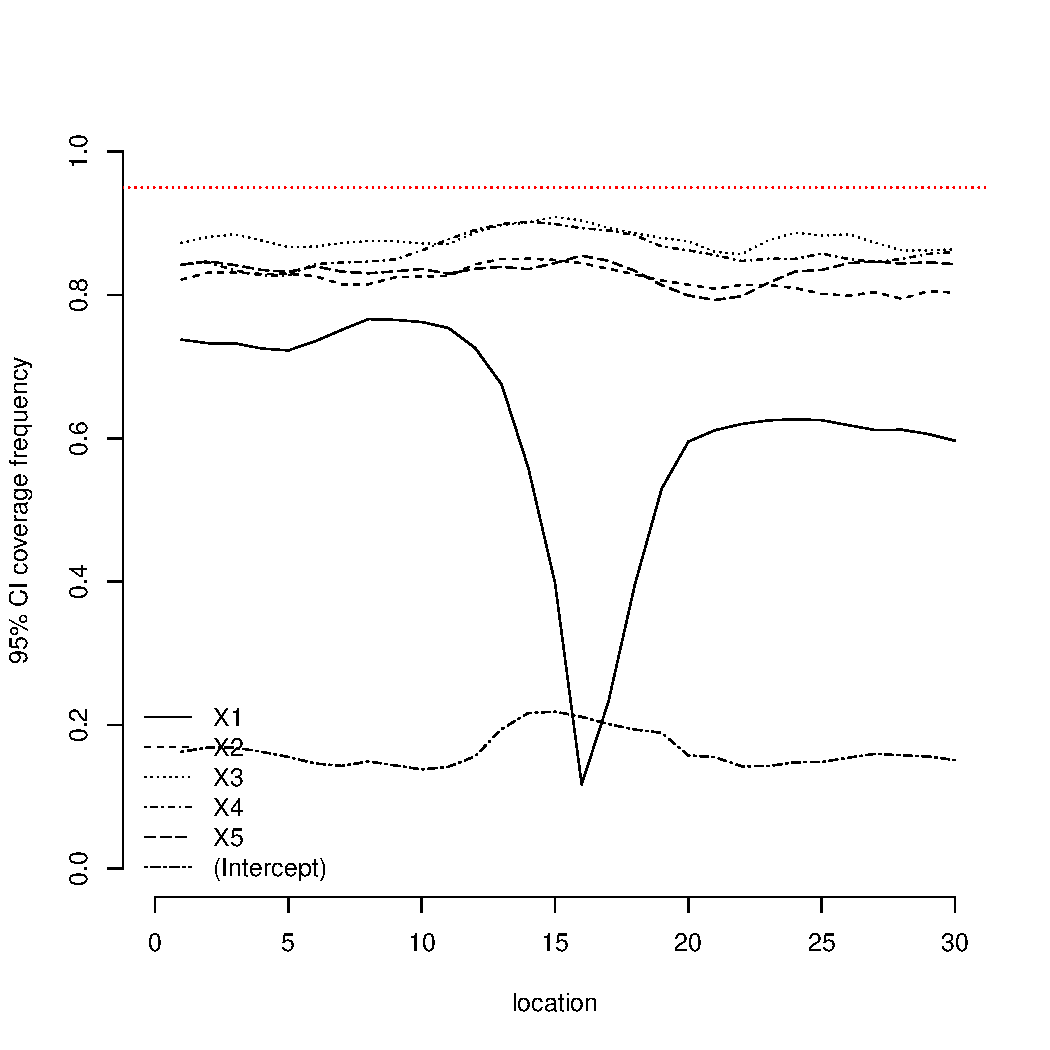
\includegraphics[width=\textwidth]{../../figures/simulation/15.5.profile_unshrunk_bootstrap_coverage.pdf}
		\caption{Unshrunk bootstrap CI coverage}
		%\label{fig:gull}
	\end{subfigure}%
	~ %add desired spacing between images, e. g. ~, \quad, \qquad etc. 
	%(or a blank line to force the subfigure onto a new line)
	\begin{subfigure}[b]{0.45\textwidth}
	\centering
		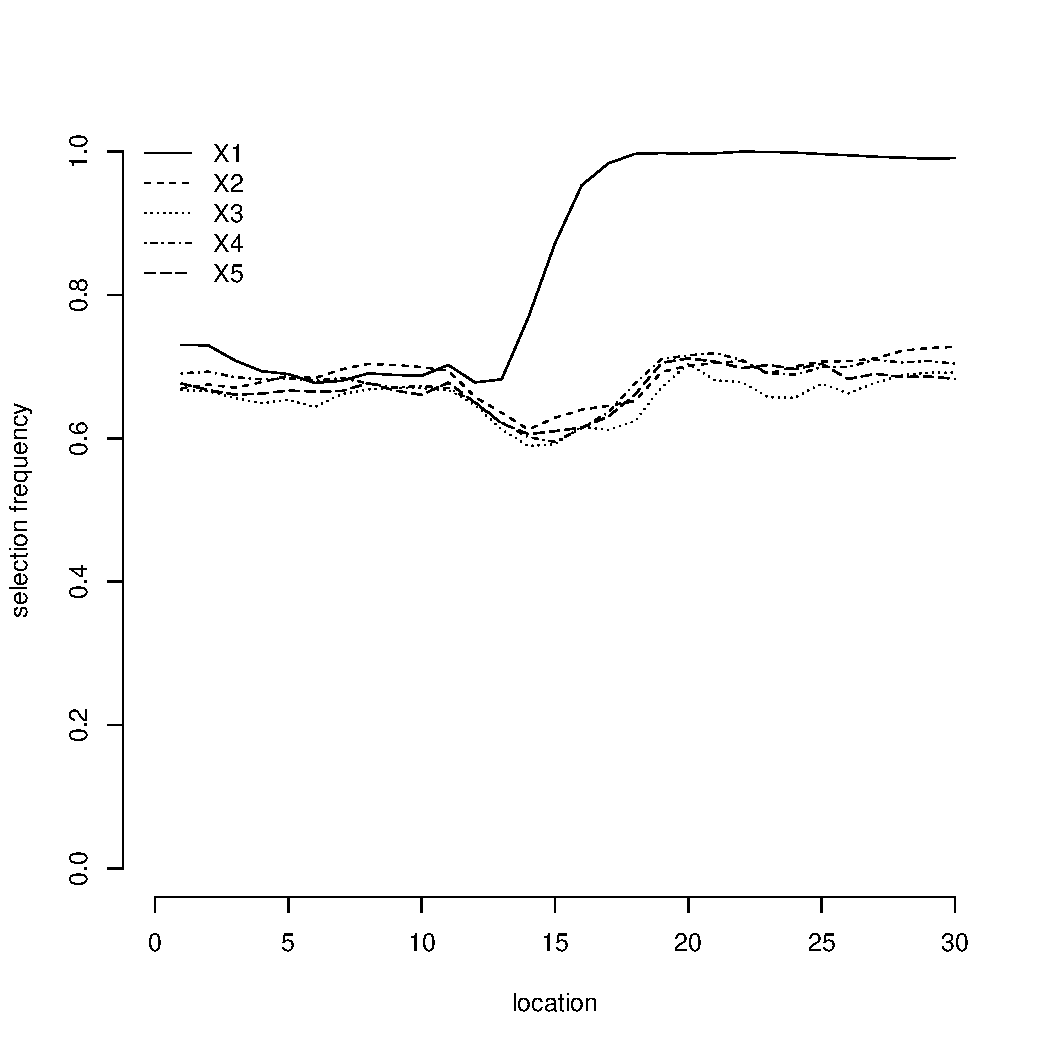
\includegraphics[width=\textwidth]{../../figures/simulation/15.5.profile_selection.pdf}
		\caption{Selection frequency}
		%\label{fig:gull}
	\end{subfigure}
	\begin{subfigure}[b]{0.45\textwidth}
	\centering
		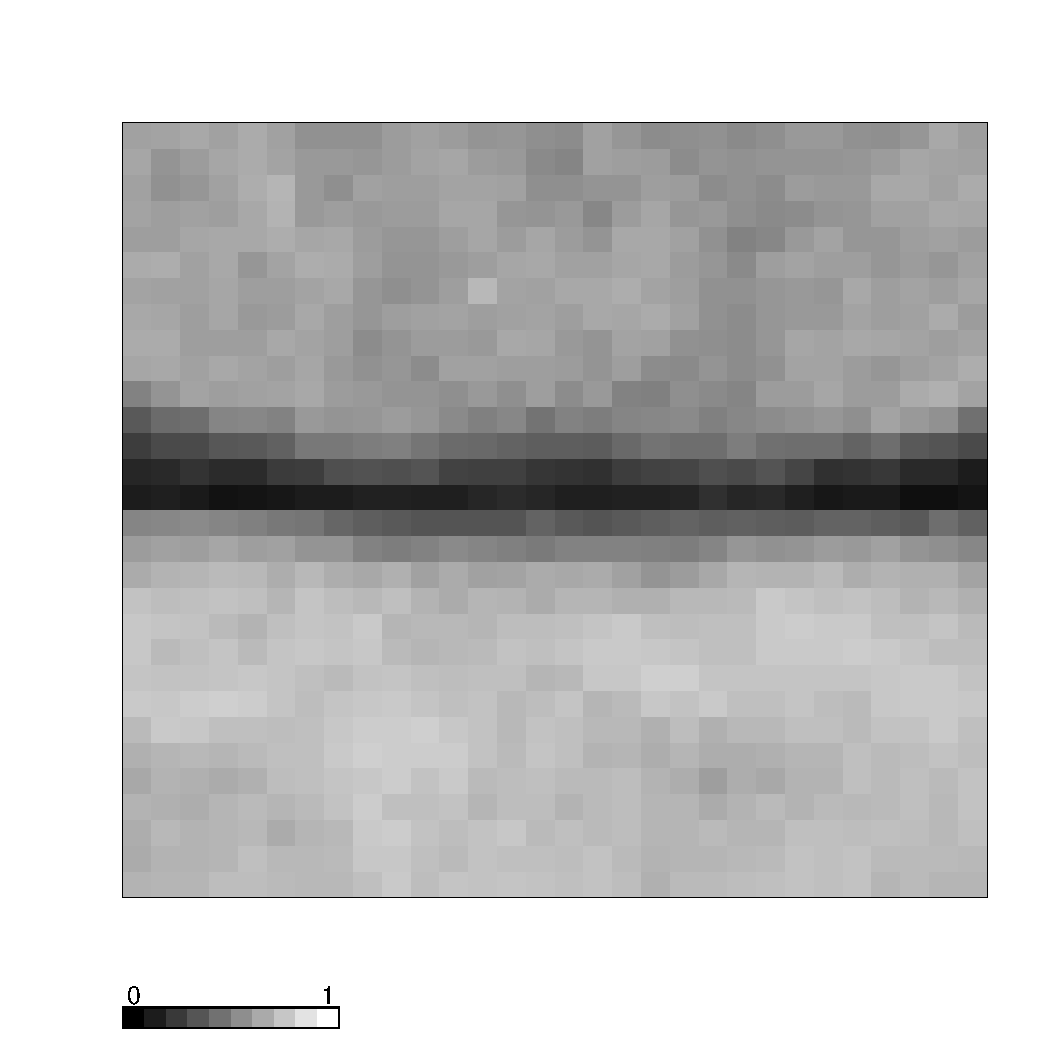
\includegraphics[width=\textwidth]{../../figures/simulation/X1.15.5.unshrunk_bootstrap_coverage.pdf}
		\caption{Unshrunk bootstrap CI coverage}
		%\label{fig:gull}
	\end{subfigure}%
	~ %add desired spacing between images, e. g. ~, \quad, \qquad etc. 
	%(or a blank line to force the subfigure onto a new line)
	\begin{subfigure}[b]{0.45\textwidth}
	\centering
		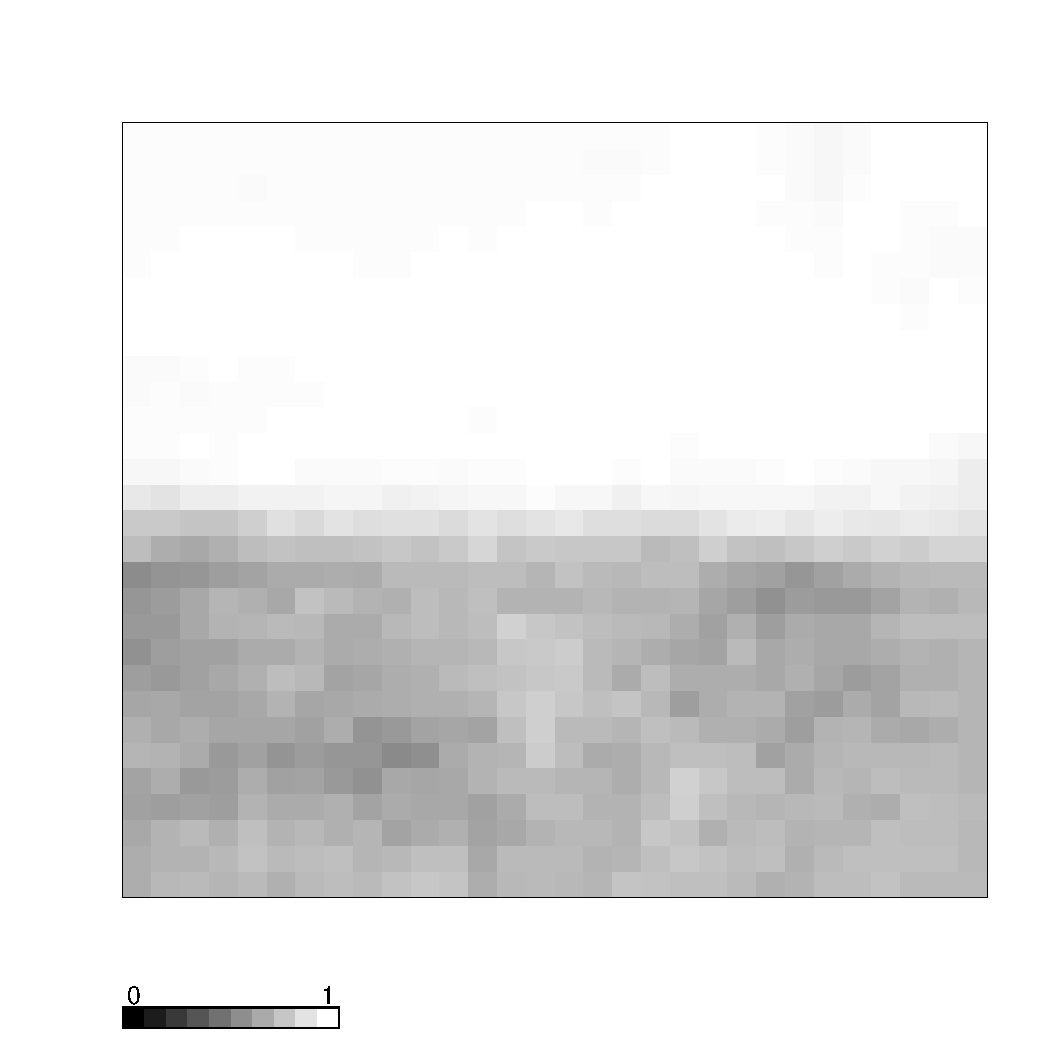
\includegraphics[width=\textwidth]{../../figures/simulation/X1.15.5.selection.pdf}
		\caption{Selection frequency}
		%\label{fig:gull}
	\end{subfigure}
	\caption{Simulation setting 5}
\end{figure}

\clearpage

\begin{figure}
	\vspace{-30mm}
	\centering
	\begin{subfigure}[b]{0.45\textwidth}
	\centering
		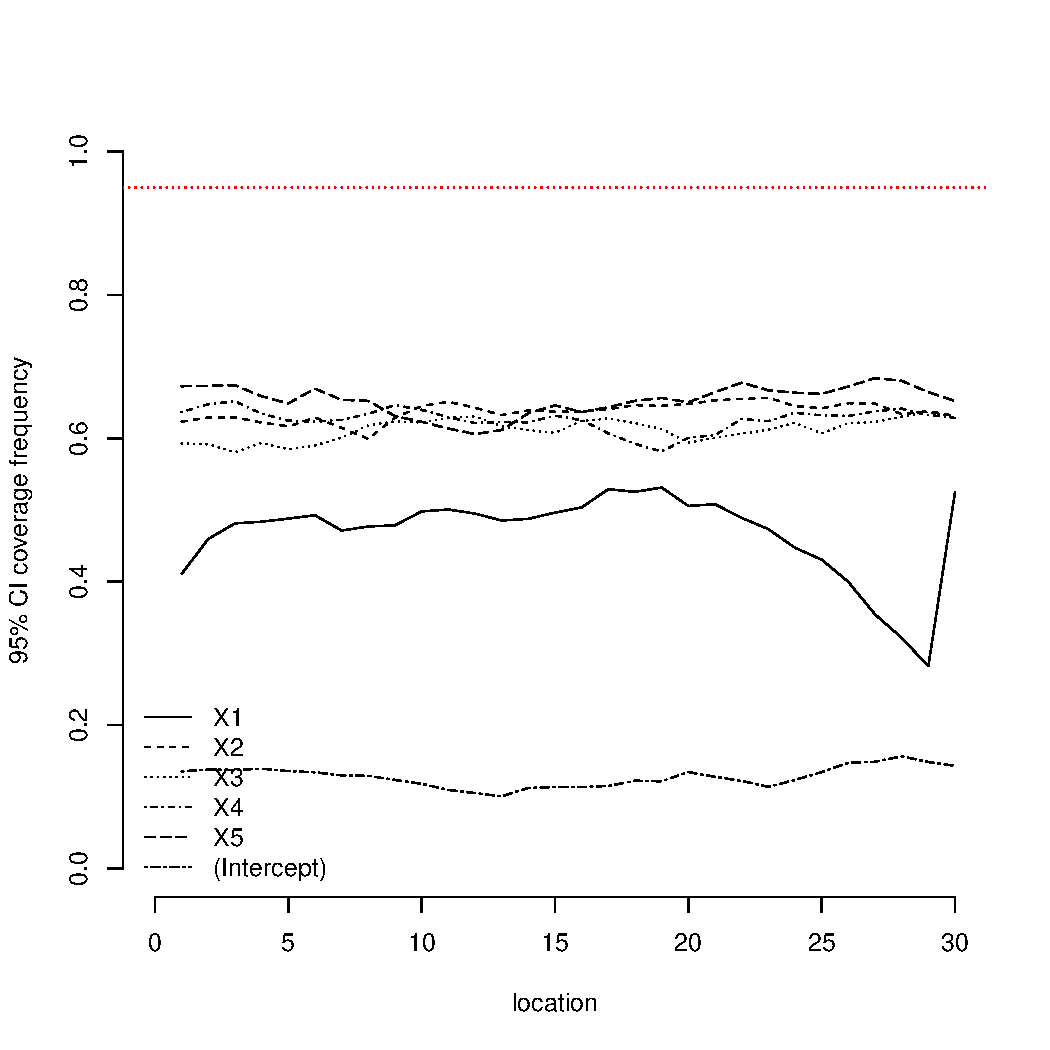
\includegraphics[width=\textwidth]{../../figures/simulation/15.6.profile_bootstrap_coverage.pdf}
		\caption{Bootstrap CI coverage}
		%\label{fig:gull}
	\end{subfigure}%
	~ %add desired spacing between images, e. g. ~, \quad, \qquad etc. 
	%(or a blank line to force the subfigure onto a new line)
	\begin{subfigure}[b]{0.45\textwidth}
	\centering
		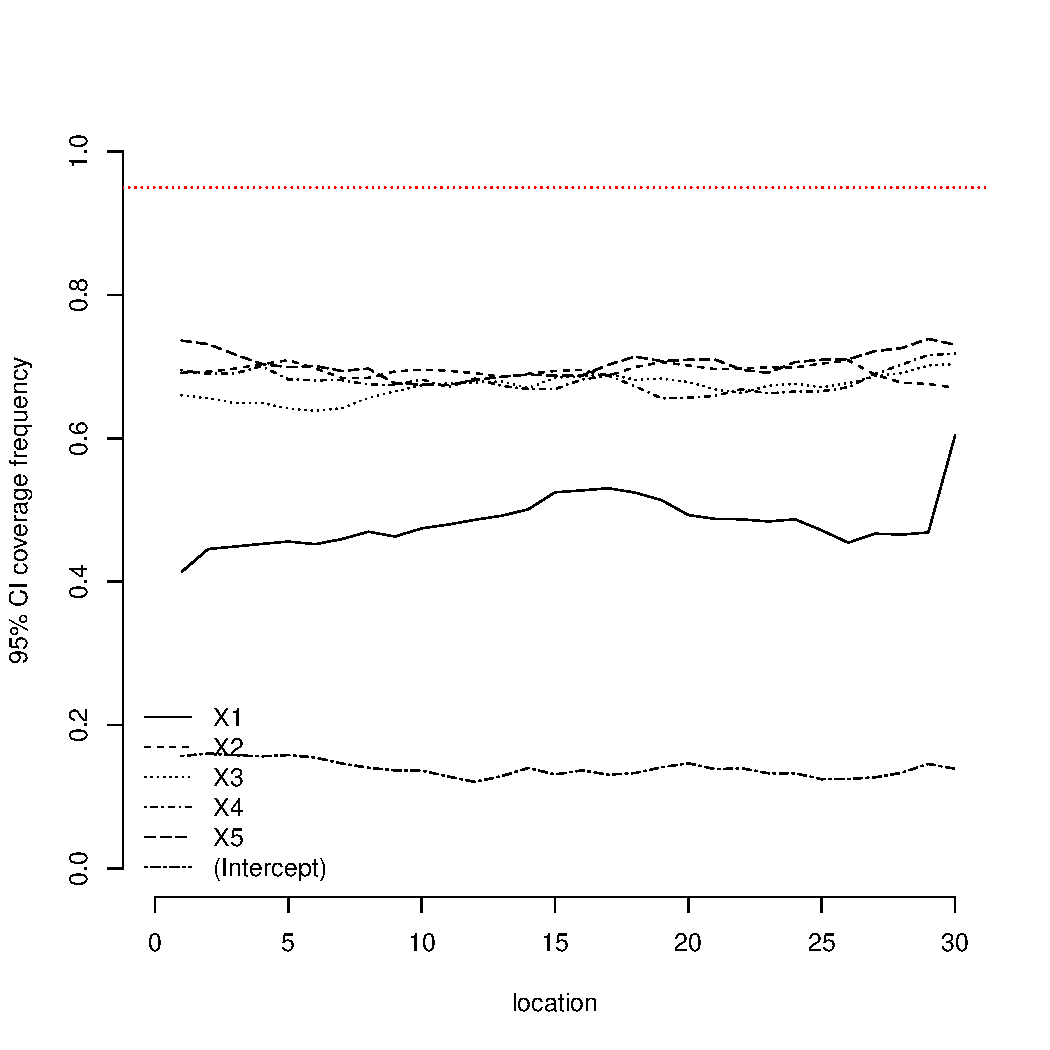
\includegraphics[width=\textwidth]{../../figures/simulation/15.6.profile_se_coverage.pdf}
		\caption{SE CI coverage}
		%\label{fig:gull}
	\end{subfigure}%
	\\%add desired spacing between images, e. g. ~, \quad, \qquad etc. 
          %(or a blank line to force the subfigure onto a new line)
	\begin{subfigure}[b]{0.45\textwidth}
	\centering
		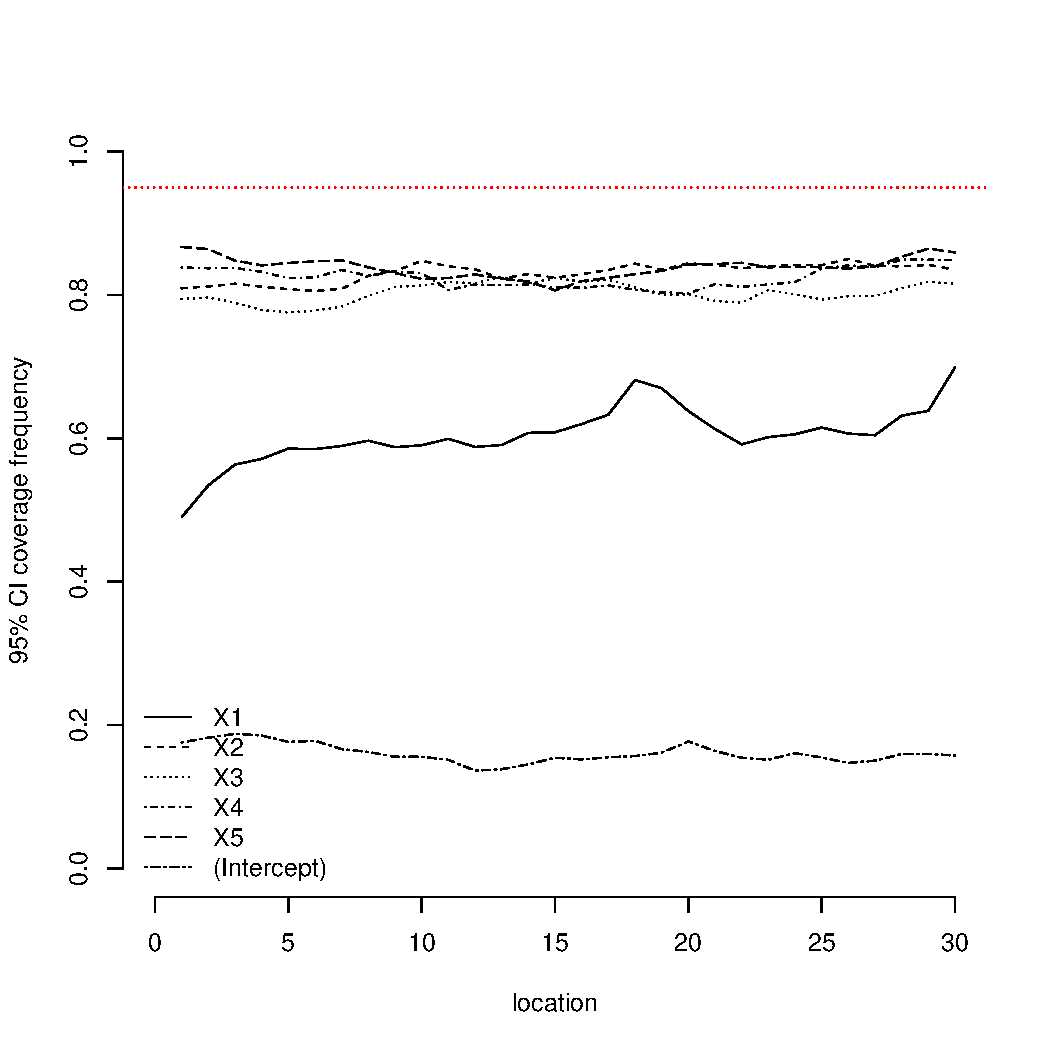
\includegraphics[width=\textwidth]{../../figures/simulation/15.6.profile_unshrunk_bootstrap_coverage.pdf}
		\caption{Unshrunk bootstrap CI coverage}
		%\label{fig:gull}
	\end{subfigure}%
	~ %add desired spacing between images, e. g. ~, \quad, \qquad etc. 
	%(or a blank line to force the subfigure onto a new line)
	\begin{subfigure}[b]{0.45\textwidth}
	\centering
		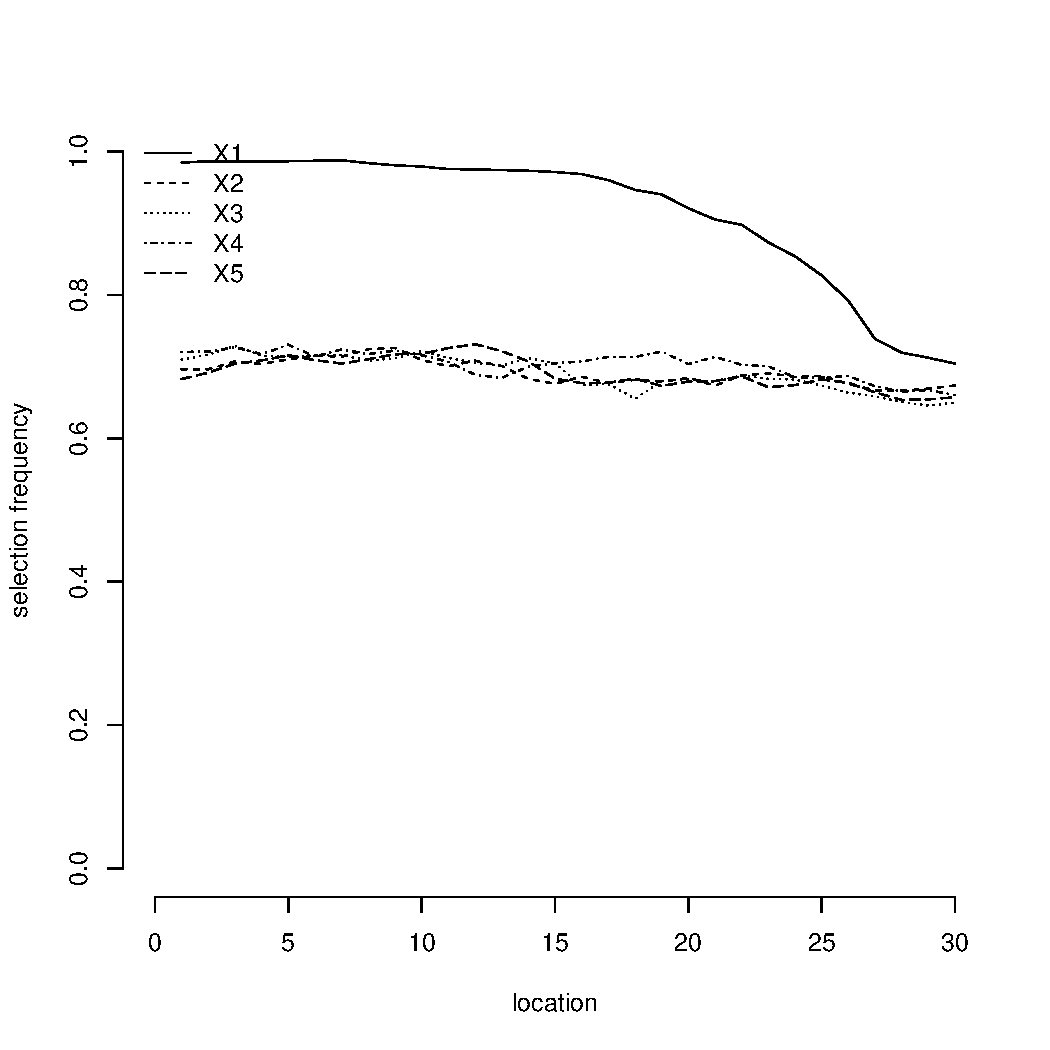
\includegraphics[width=\textwidth]{../../figures/simulation/15.6.profile_selection.pdf}
		\caption{Selection frequency}
		%\label{fig:gull}
	\end{subfigure}
	\begin{subfigure}[b]{0.45\textwidth}
	\centering
		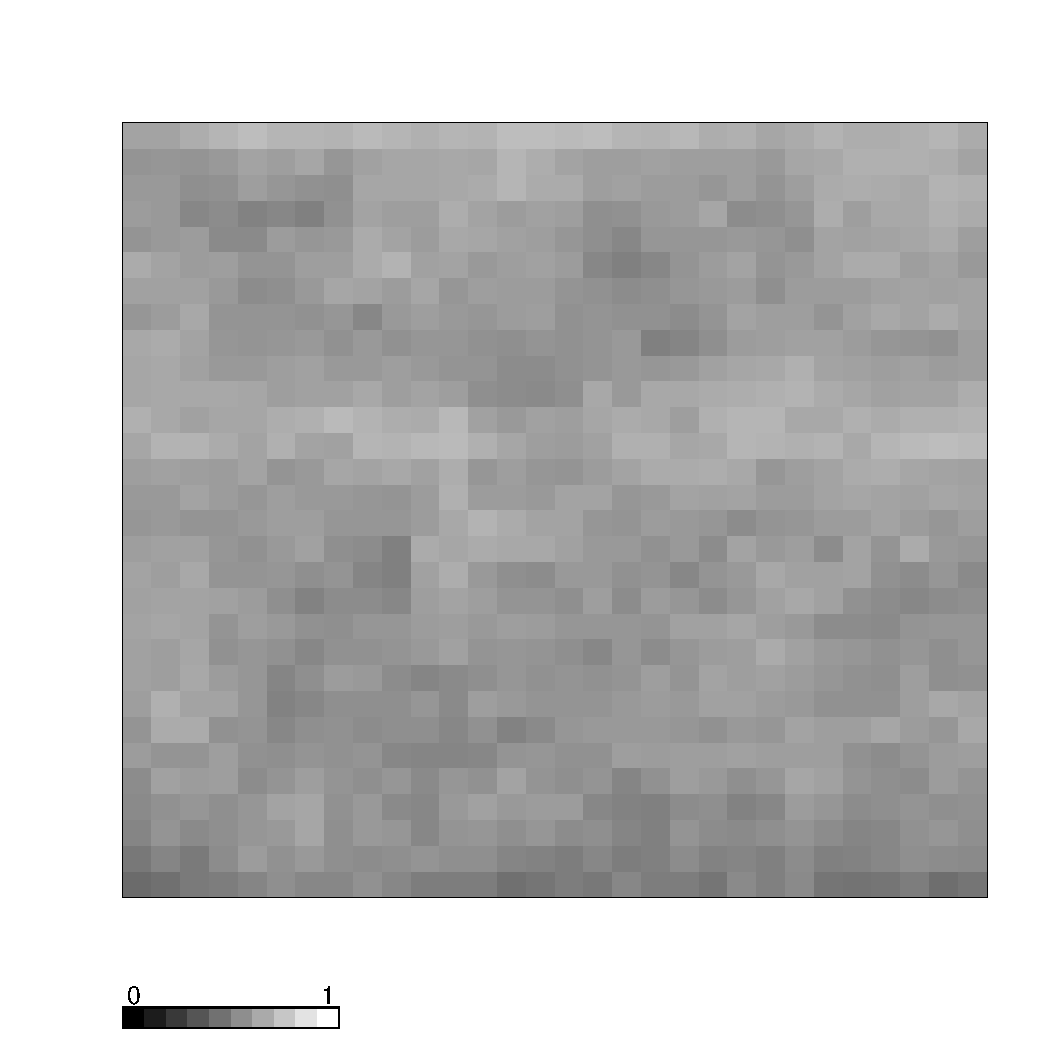
\includegraphics[width=\textwidth]{../../figures/simulation/X1.15.6.unshrunk_bootstrap_coverage.pdf}
		\caption{Unshrunk bootstrap CI coverage}
		%\label{fig:gull}
	\end{subfigure}%
	~ %add desired spacing between images, e. g. ~, \quad, \qquad etc. 
	%(or a blank line to force the subfigure onto a new line)
	\begin{subfigure}[b]{0.45\textwidth}
	\centering
		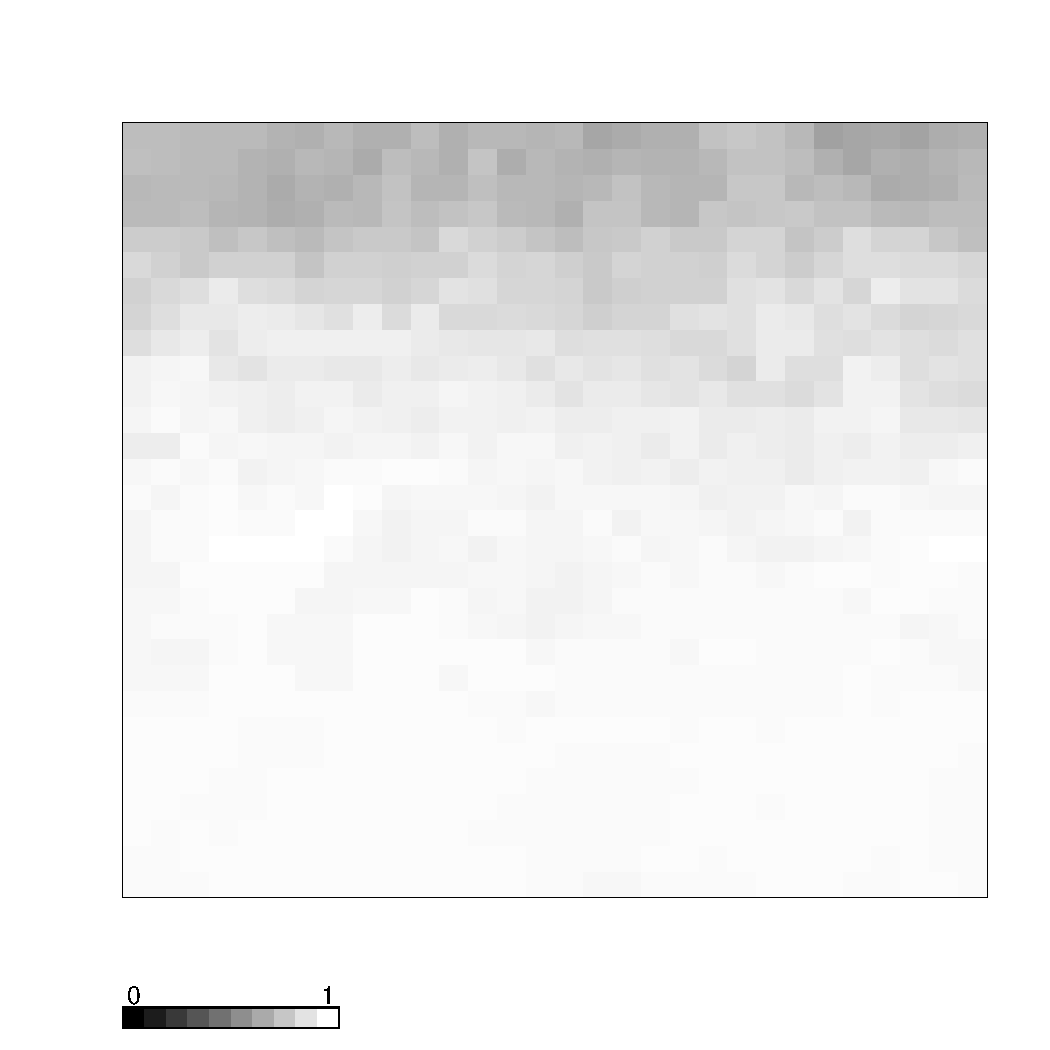
\includegraphics[width=\textwidth]{../../figures/simulation/X1.15.6.selection.pdf}
		\caption{Selection frequency}
		%\label{fig:gull}
	\end{subfigure}
	\caption{Simulation setting 6}
\end{figure}

\clearpage

\begin{figure}
	\vspace{-30mm}
	\centering
	\begin{subfigure}[b]{0.45\textwidth}
	\centering
		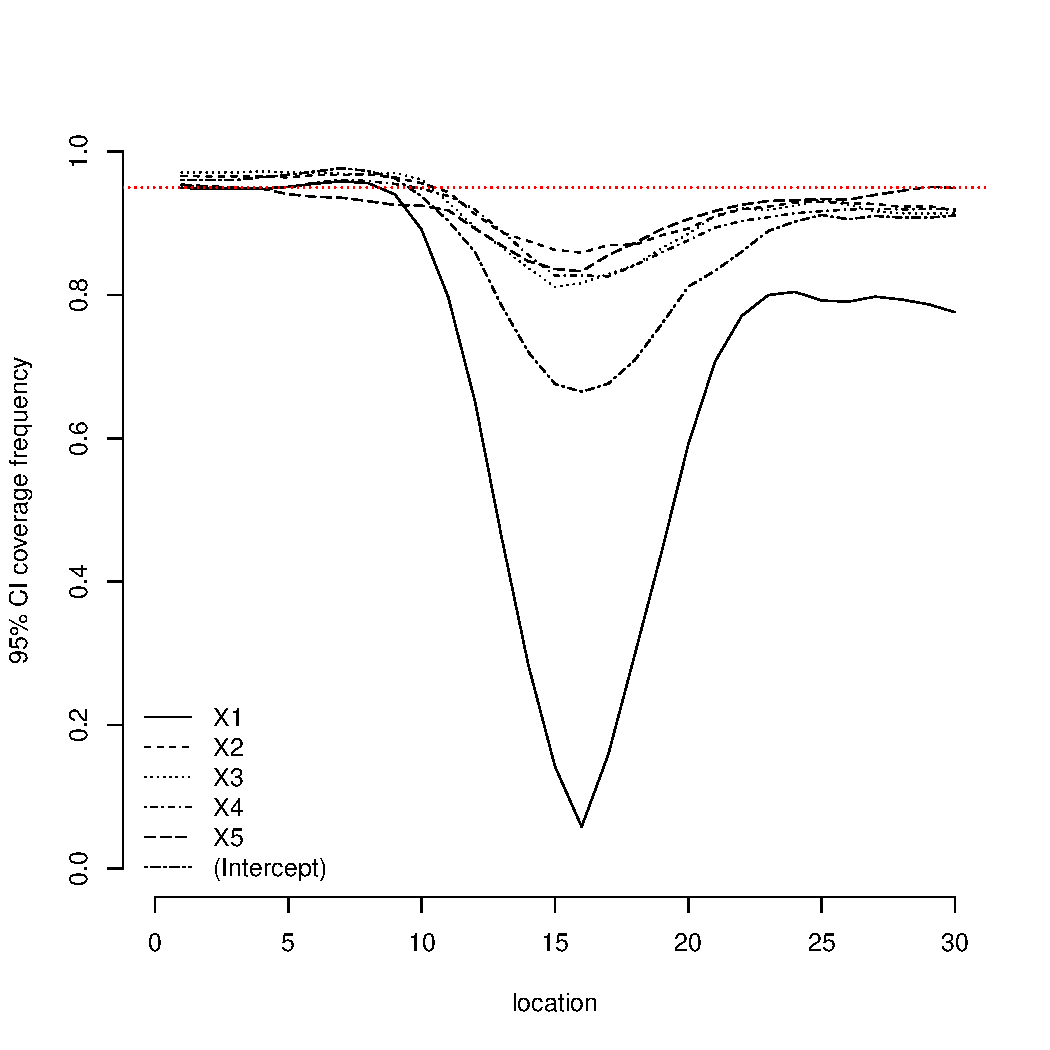
\includegraphics[width=\textwidth]{../../figures/simulation/15.7.profile_bootstrap_coverage.pdf}
		\caption{Bootstrap CI coverage}
		%\label{fig:gull}
	\end{subfigure}%
	~ %add desired spacing between images, e. g. ~, \quad, \qquad etc. 
	%(or a blank line to force the subfigure onto a new line)
	\begin{subfigure}[b]{0.45\textwidth}
	\centering
		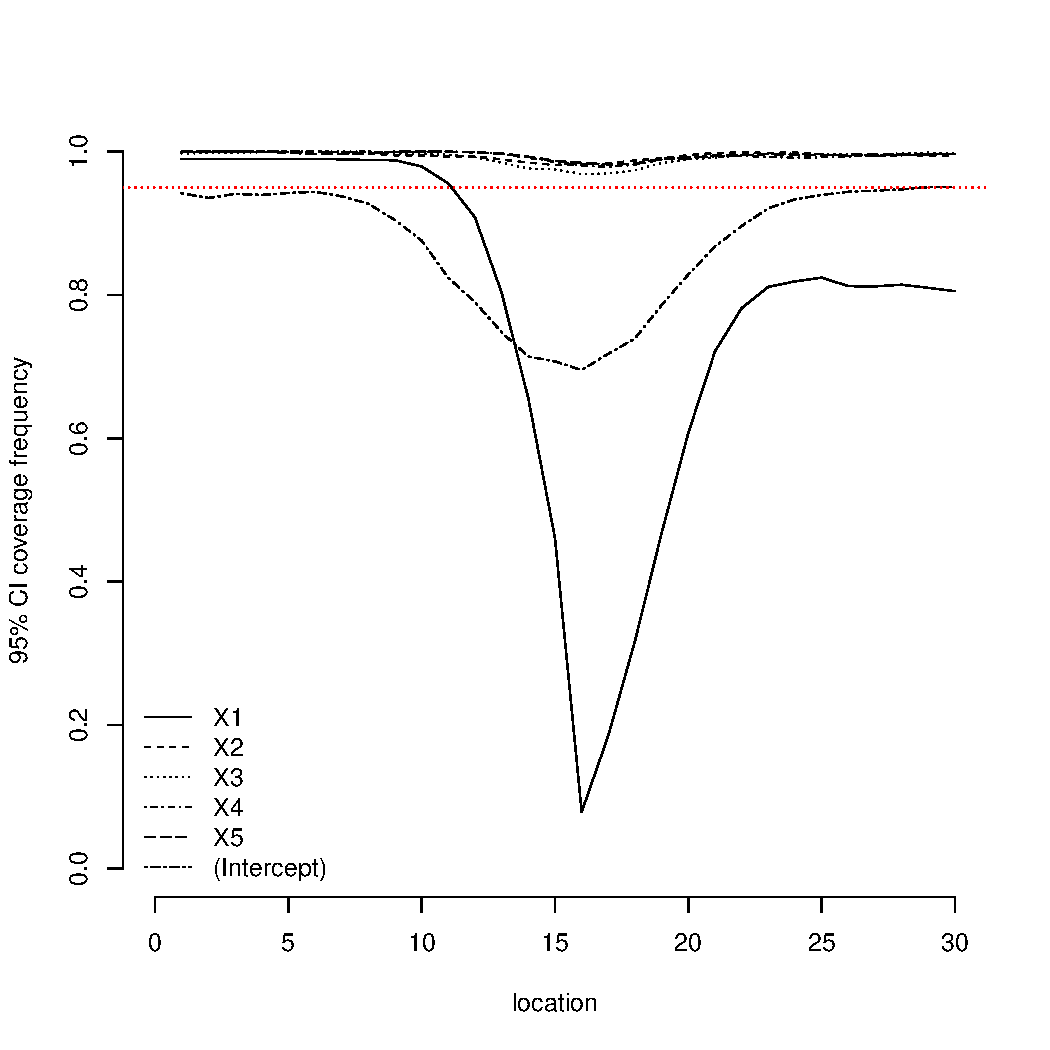
\includegraphics[width=\textwidth]{../../figures/simulation/15.7.profile_se_coverage.pdf}
		\caption{SE CI coverage}
		%\label{fig:gull}
	\end{subfigure}%
	\\%add desired spacing between images, e. g. ~, \quad, \qquad etc. 
          %(or a blank line to force the subfigure onto a new line)
	\begin{subfigure}[b]{0.45\textwidth}
	\centering
		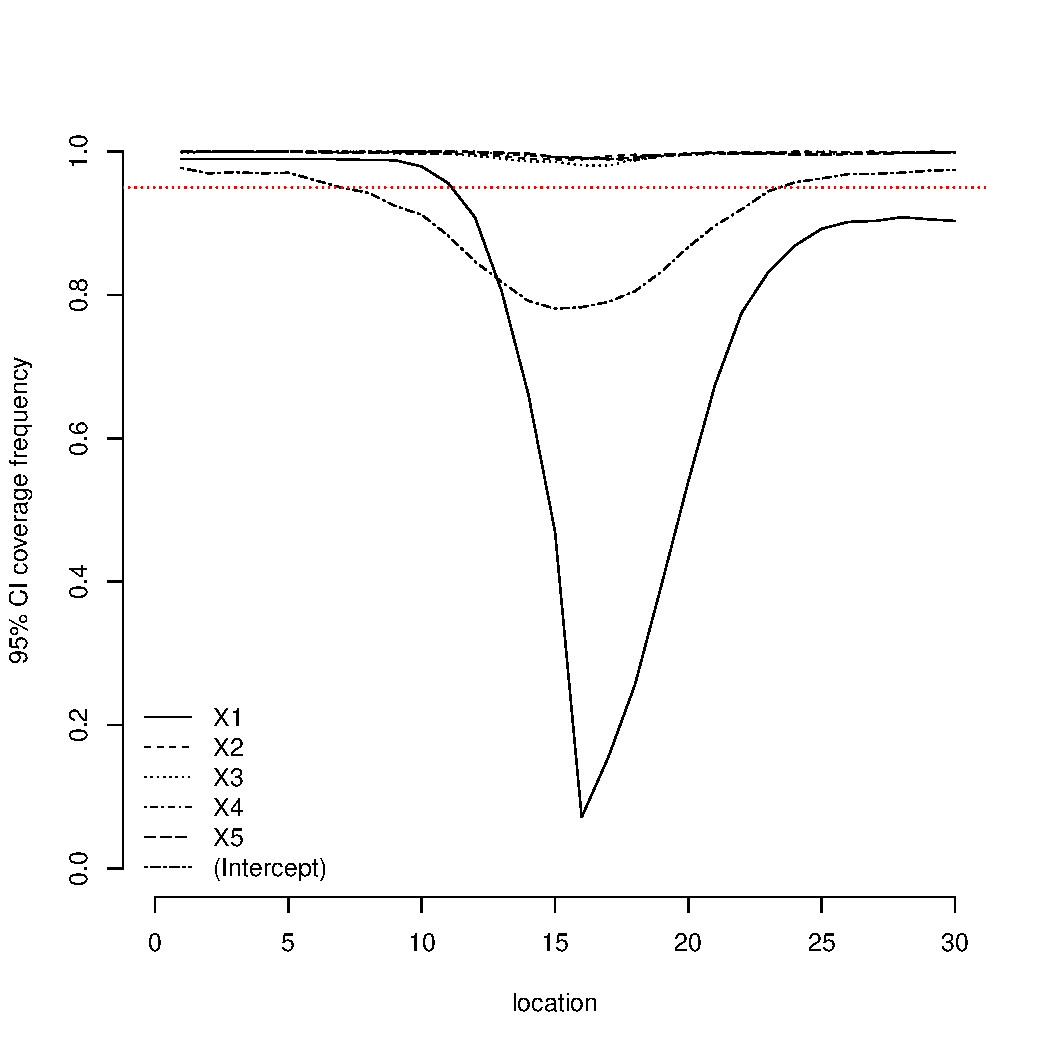
\includegraphics[width=\textwidth]{../../figures/simulation/15.7.profile_unshrunk_bootstrap_coverage.pdf}
		\caption{Unshrunk bootstrap CI coverage}
		%\label{fig:gull}
	\end{subfigure}%
	~ %add desired spacing between images, e. g. ~, \quad, \qquad etc. 
	%(or a blank line to force the subfigure onto a new line)
	\begin{subfigure}[b]{0.45\textwidth}
	\centering
		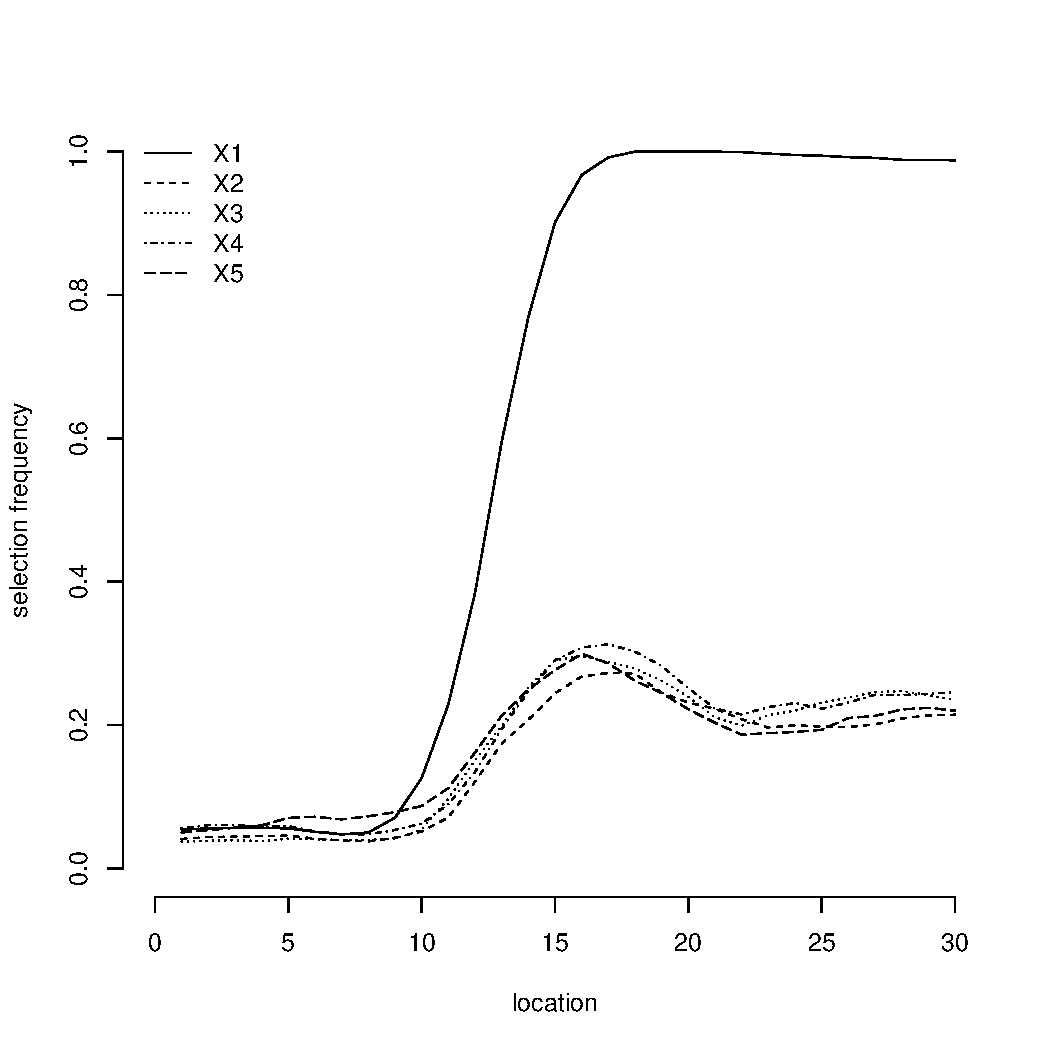
\includegraphics[width=\textwidth]{../../figures/simulation/15.7.profile_selection.pdf}
		\caption{Selection frequency}
		%\label{fig:gull}
	\end{subfigure}
	\begin{subfigure}[b]{0.45\textwidth}
	\centering
		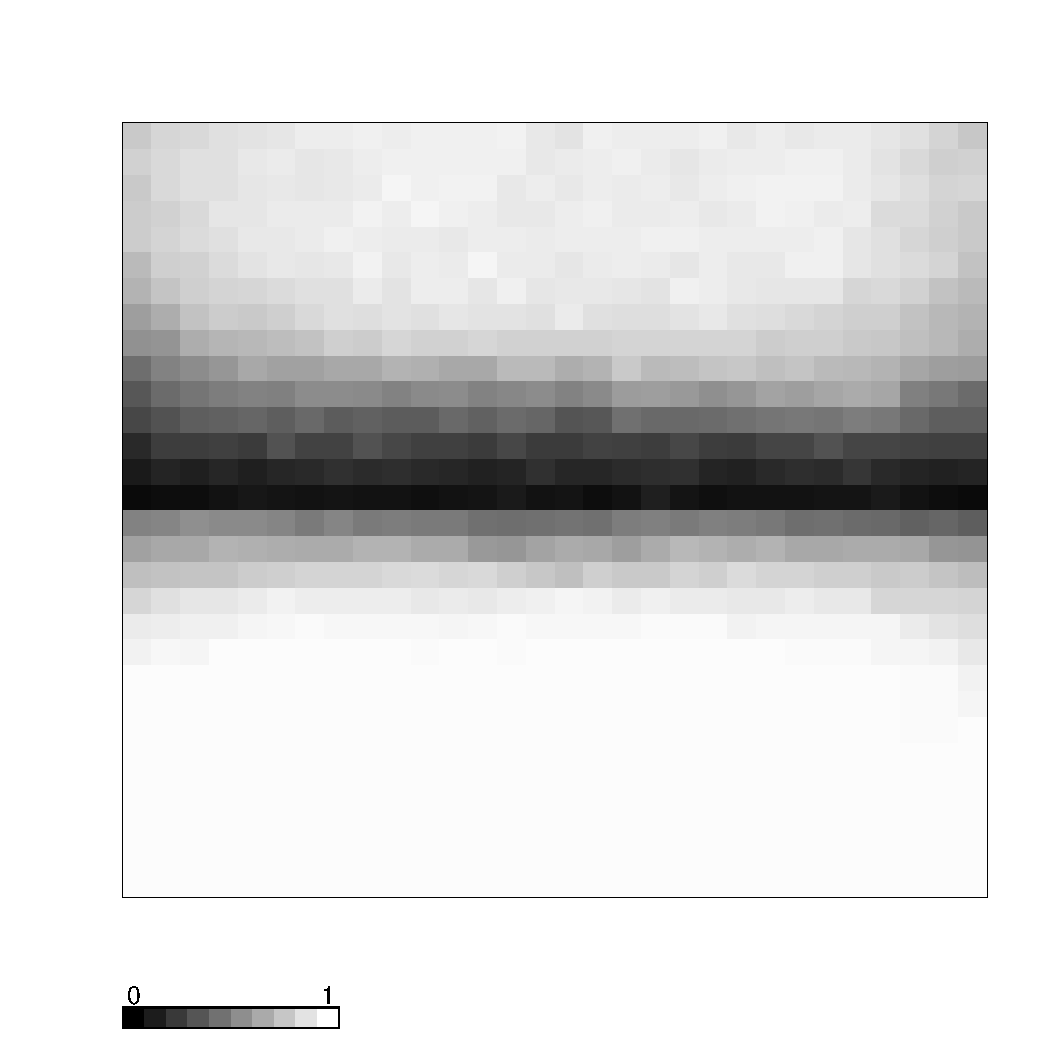
\includegraphics[width=\textwidth]{../../figures/simulation/X1.15.7.unshrunk_bootstrap_coverage.pdf}
		\caption{Unshrunk bootstrap CI coverage}
		%\label{fig:gull}
	\end{subfigure}%
	~ %add desired spacing between images, e. g. ~, \quad, \qquad etc. 
	%(or a blank line to force the subfigure onto a new line)
	\begin{subfigure}[b]{0.45\textwidth}
	\centering
		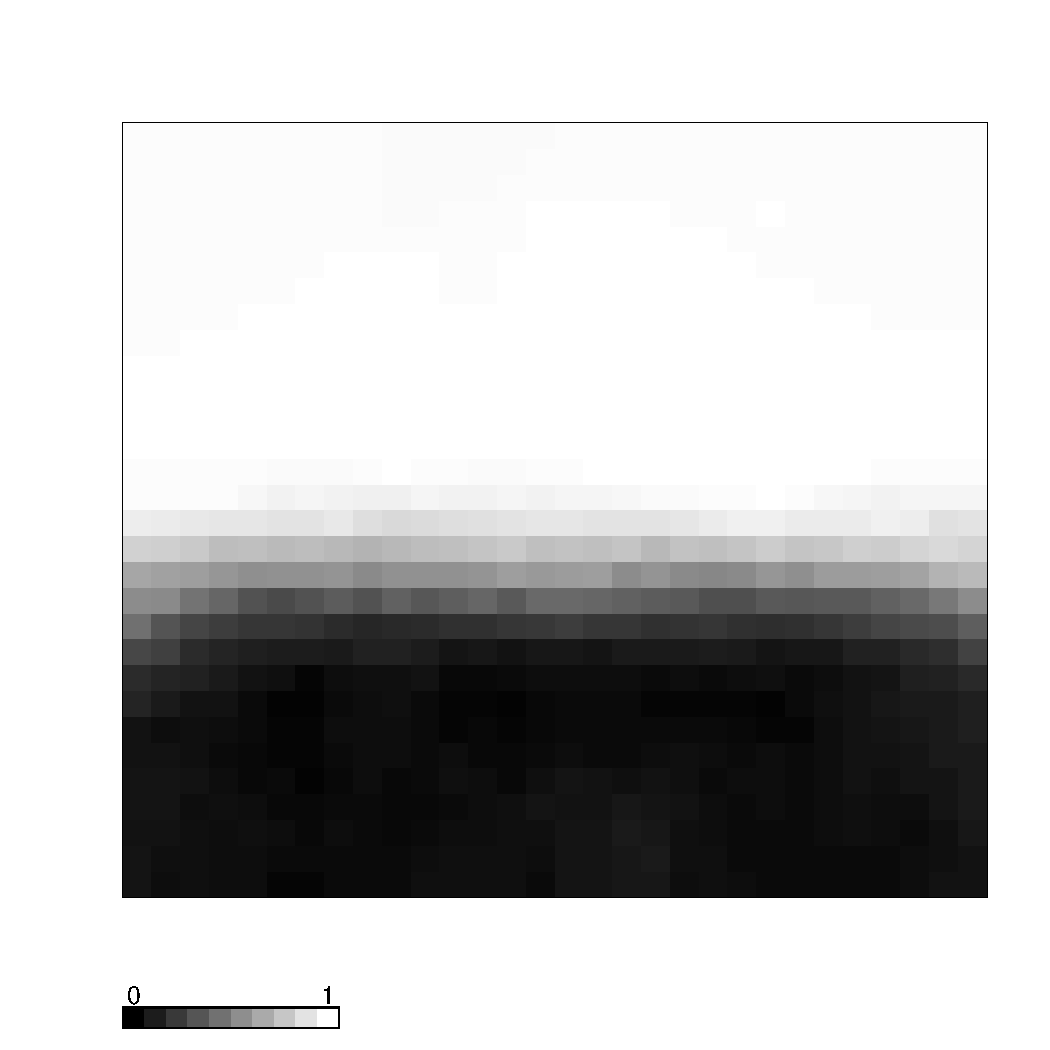
\includegraphics[width=\textwidth]{../../figures/simulation/X1.15.7.selection.pdf}
		\caption{Selection frequency}
		%\label{fig:gull}
	\end{subfigure}
	\caption{Simulation setting 7}
\end{figure}
	
\clearpage

\begin{figure}
	\vspace{-30mm}
	\centering
	\begin{subfigure}[b]{0.45\textwidth}
	\centering
		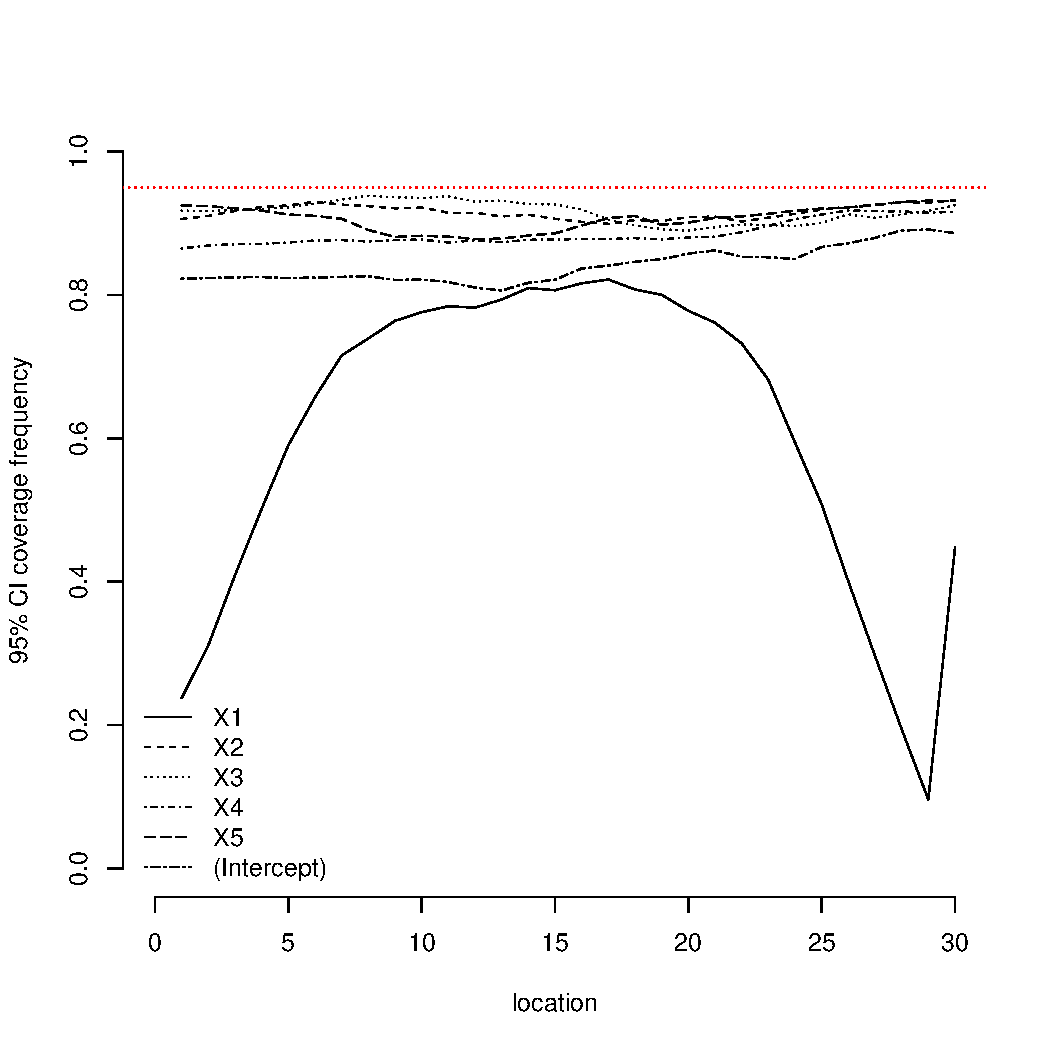
\includegraphics[width=\textwidth]{../../figures/simulation/15.8.profile_bootstrap_coverage.pdf}
		\caption{Bootstrap CI coverage}
		%\label{fig:gull}
	\end{subfigure}%
	~ %add desired spacing between images, e. g. ~, \quad, \qquad etc. 
	%(or a blank line to force the subfigure onto a new line)
	\begin{subfigure}[b]{0.45\textwidth}
	\centering
		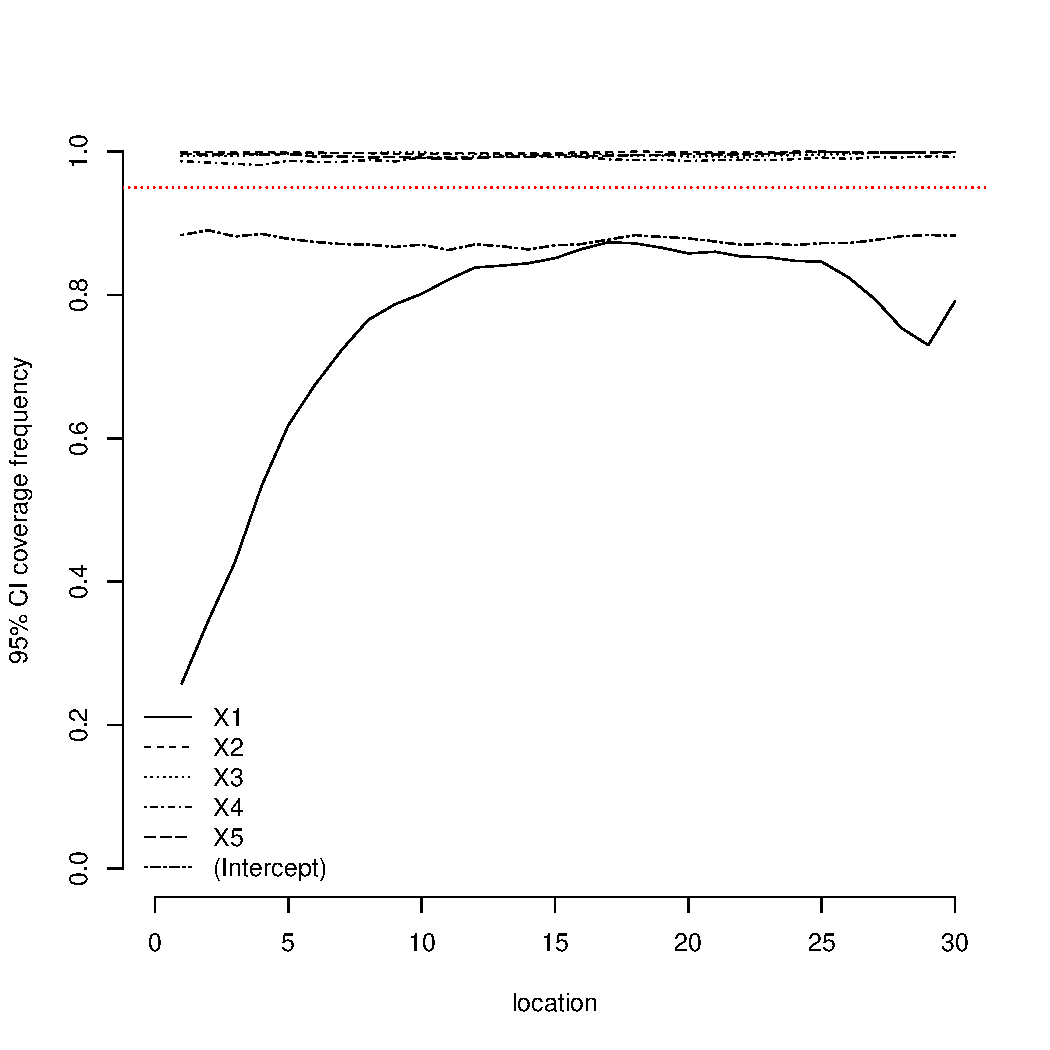
\includegraphics[width=\textwidth]{../../figures/simulation/15.8.profile_se_coverage.pdf}
		\caption{SE CI coverage}
		%\label{fig:gull}
	\end{subfigure}%
	\\%add desired spacing between images, e. g. ~, \quad, \qquad etc. 
          %(or a blank line to force the subfigure onto a new line)
	\begin{subfigure}[b]{0.45\textwidth}
	\centering
		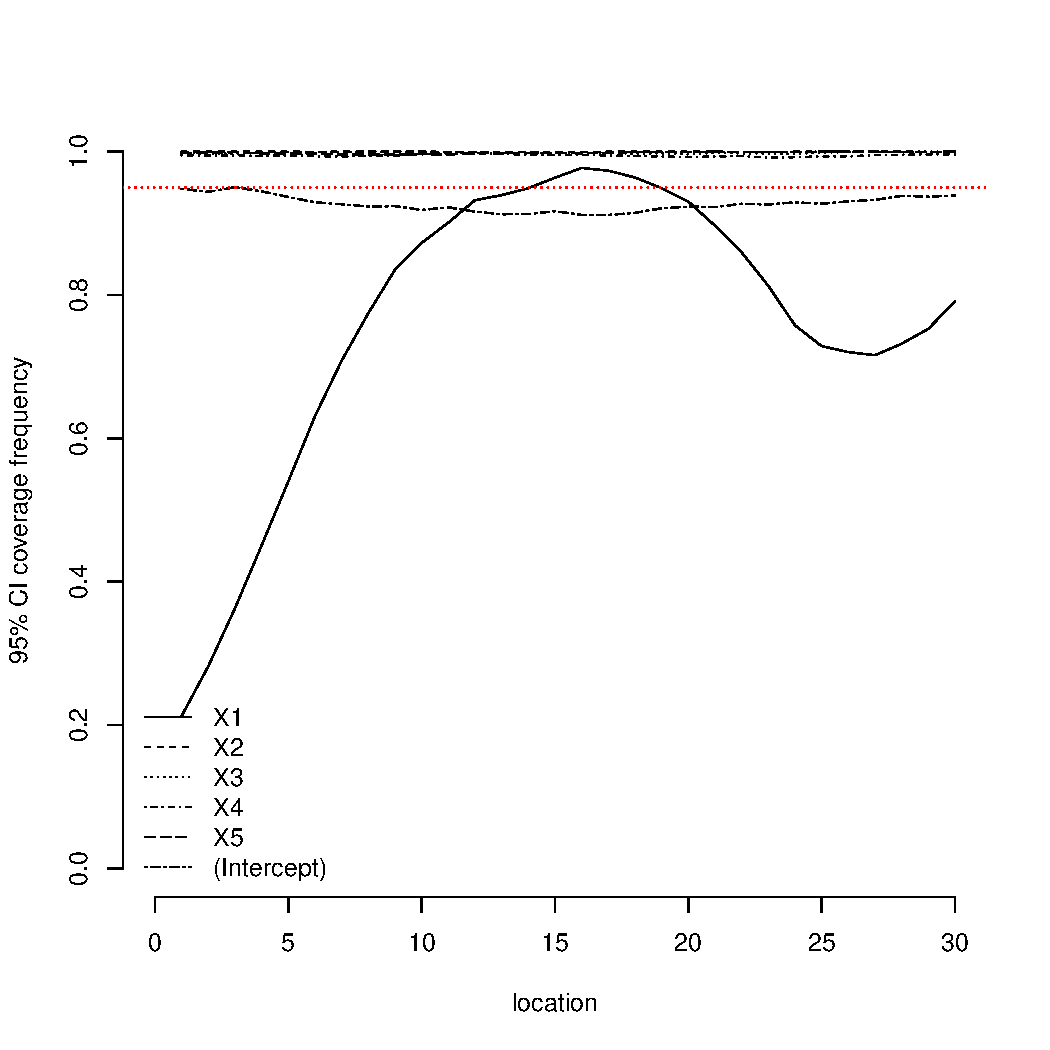
\includegraphics[width=\textwidth]{../../figures/simulation/15.8.profile_unshrunk_bootstrap_coverage.pdf}
		\caption{Unshrunk bootstrap CI coverage}
		%\label{fig:gull}
	\end{subfigure}%
	~ %add desired spacing between images, e. g. ~, \quad, \qquad etc. 
	%(or a blank line to force the subfigure onto a new line)
	\begin{subfigure}[b]{0.45\textwidth}
	\centering
		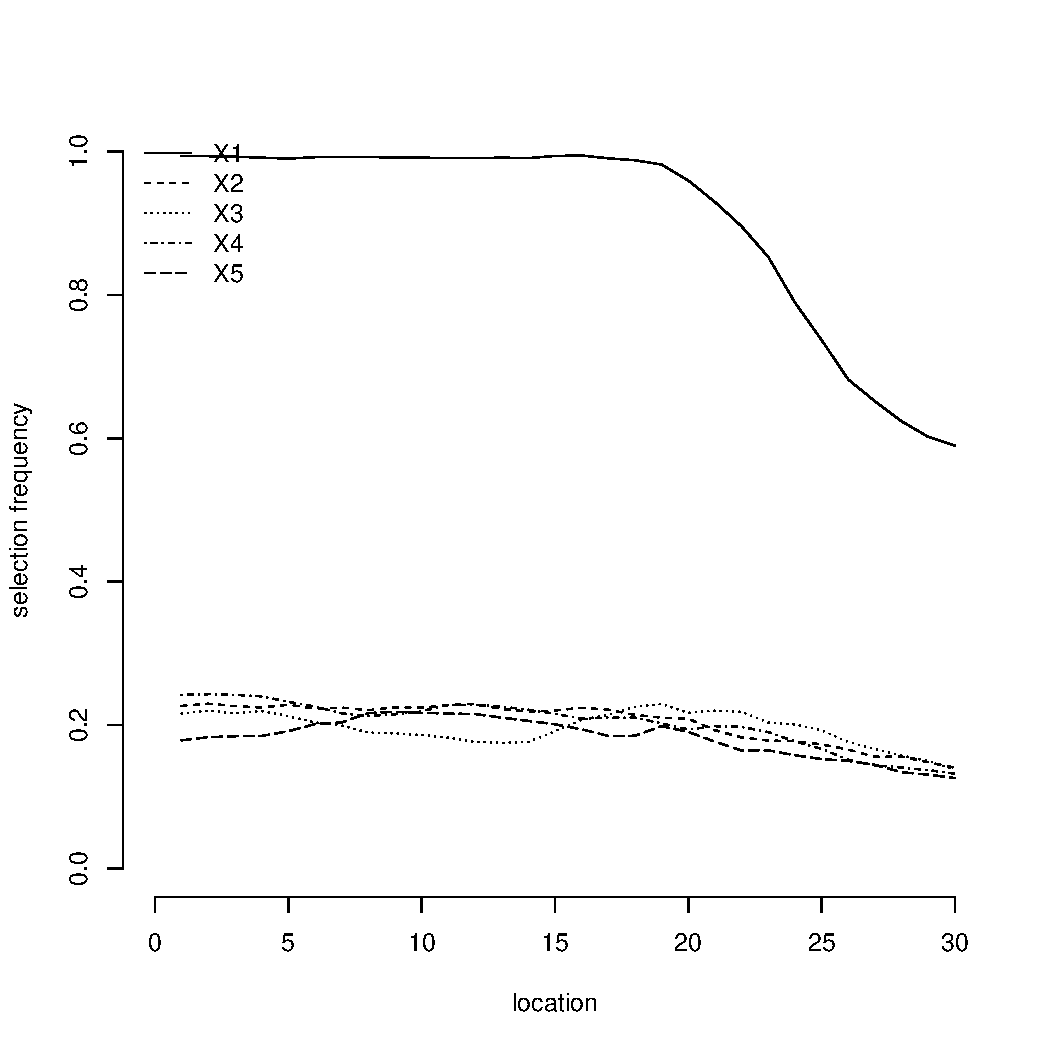
\includegraphics[width=\textwidth]{../../figures/simulation/15.8.profile_selection.pdf}
		\caption{Selection frequency}
		%\label{fig:gull}
	\end{subfigure}
	\begin{subfigure}[b]{0.45\textwidth}
	\centering
		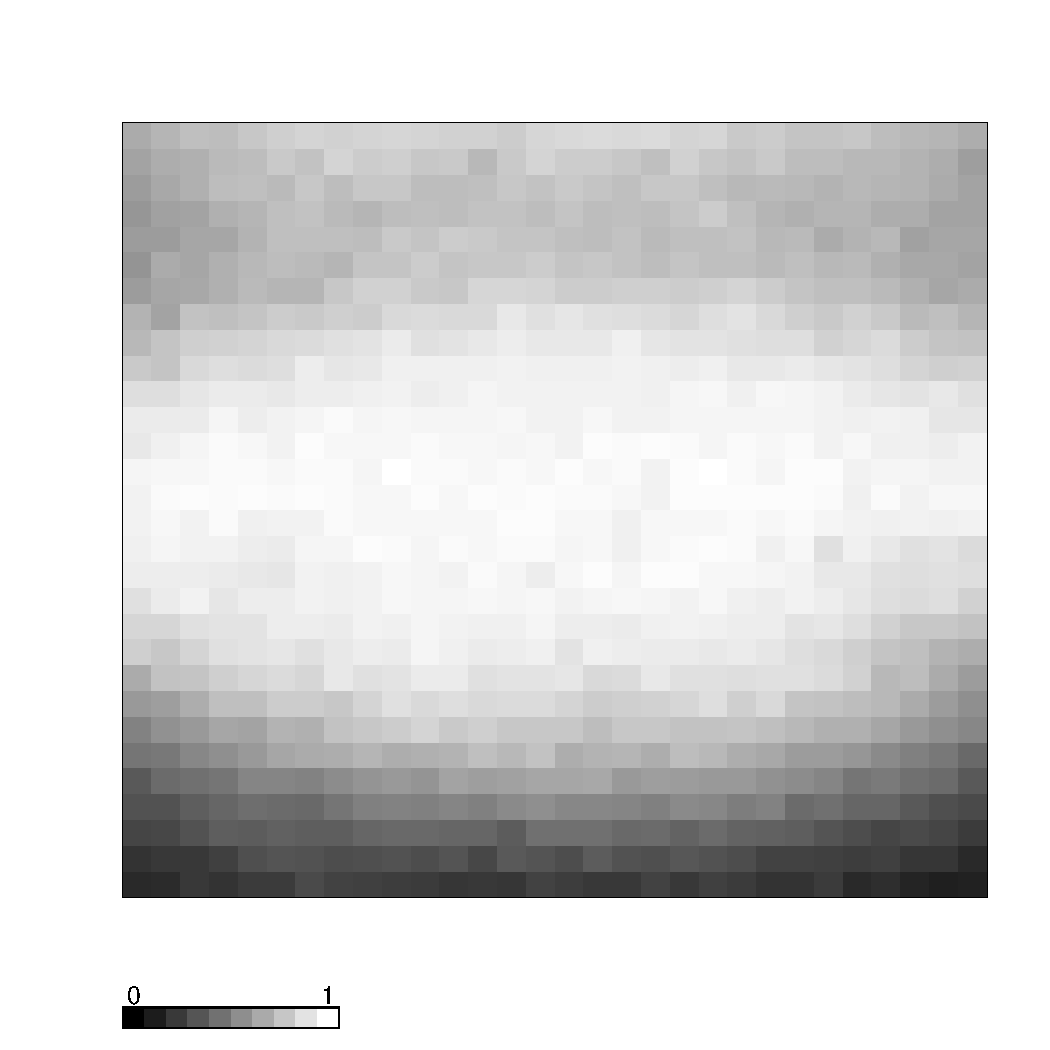
\includegraphics[width=\textwidth]{../../figures/simulation/X1.15.8.unshrunk_bootstrap_coverage.pdf}
		\caption{Unshrunk bootstrap CI coverage}
		%\label{fig:gull}
	\end{subfigure}%
	~ %add desired spacing between images, e. g. ~, \quad, \qquad etc. 
	%(or a blank line to force the subfigure onto a new line)
	\begin{subfigure}[b]{0.45\textwidth}
	\centering
		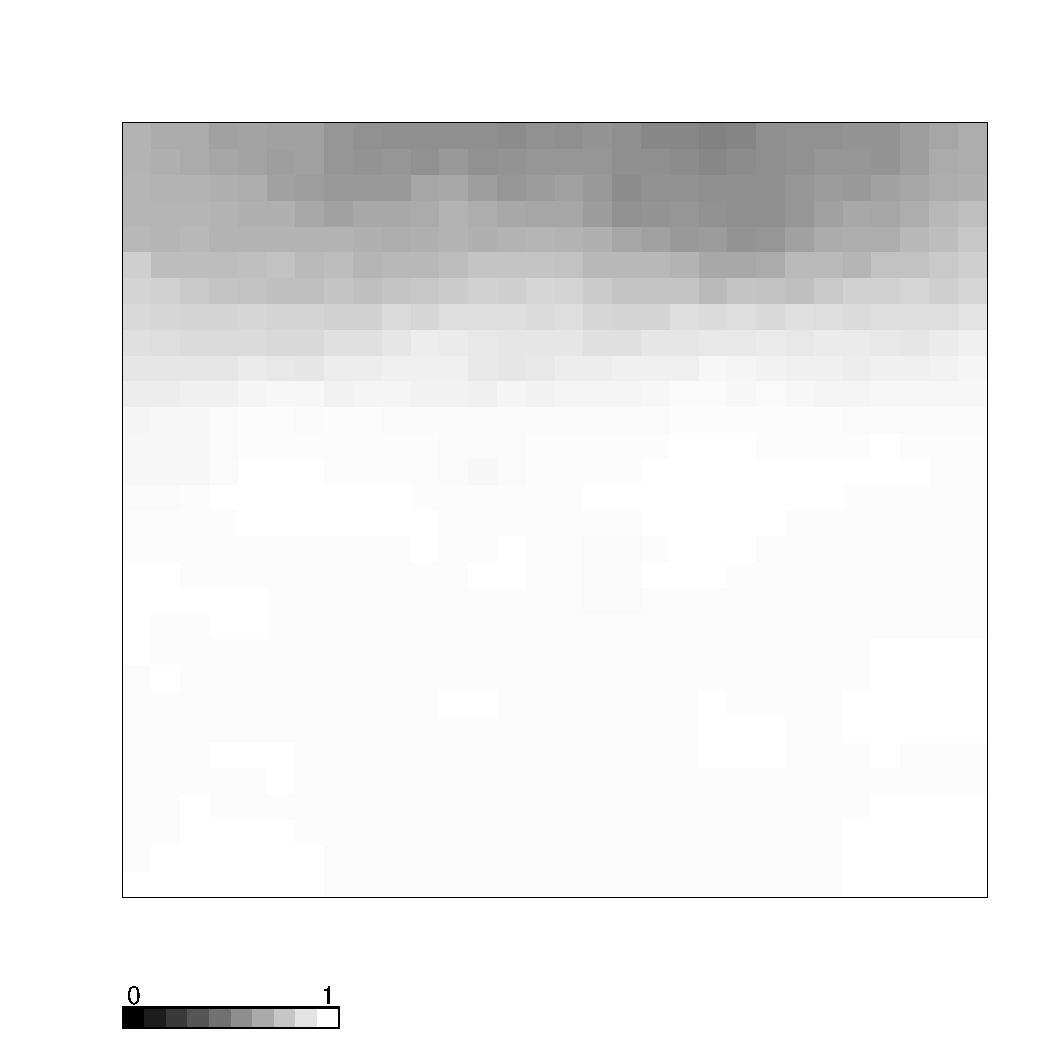
\includegraphics[width=\textwidth]{../../figures/simulation/X1.15.8.selection.pdf}
		\caption{Selection frequency}
		%\label{fig:gull}
	\end{subfigure}
	\caption{Simulation setting 8}
\end{figure}
	
	\clearpage
	
\begin{figure}
	\vspace{-30mm}
	\centering
	\begin{subfigure}[b]{0.45\textwidth}
	\centering
		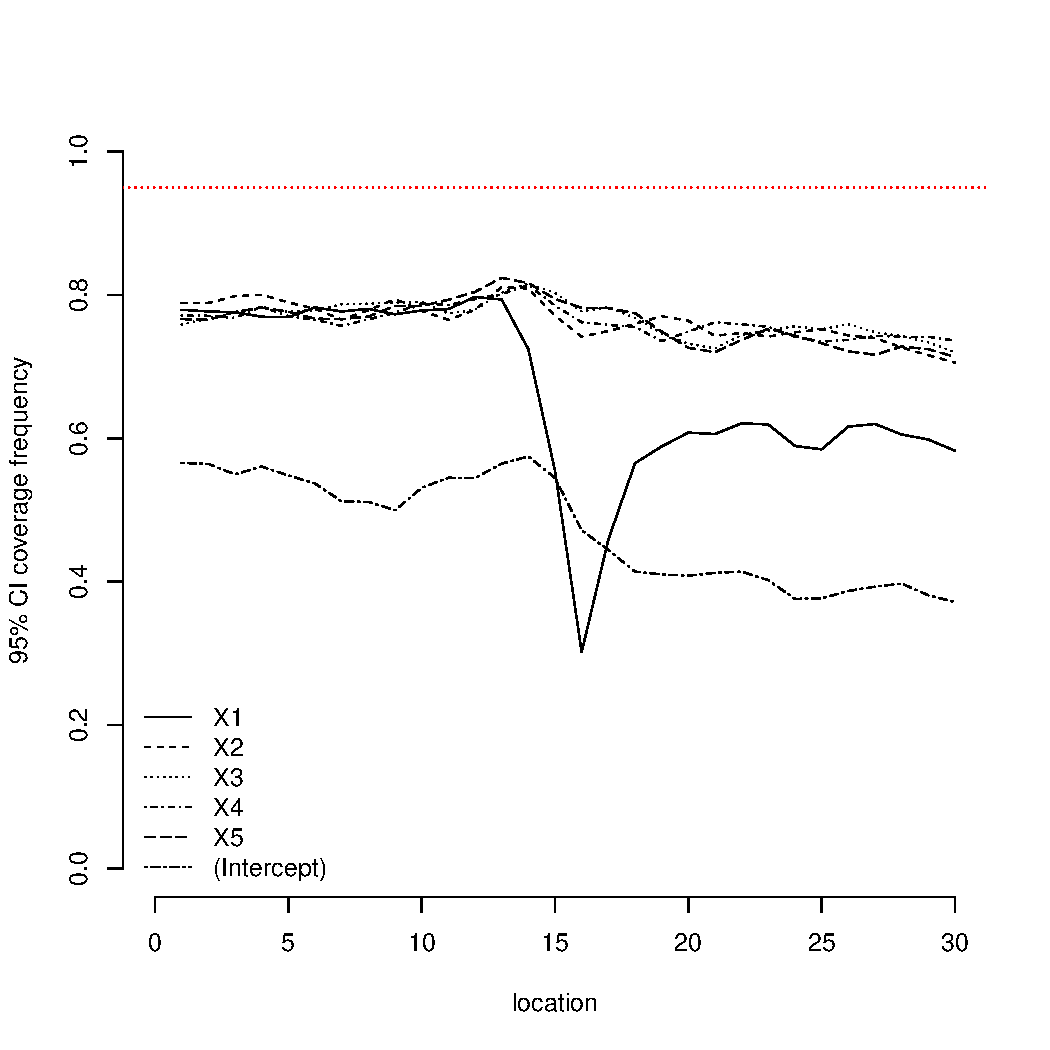
\includegraphics[width=\textwidth]{../../figures/simulation/15.9.profile_bootstrap_coverage.pdf}
		\caption{Bootstrap CI coverage}
		%\label{fig:gull}
	\end{subfigure}%
	~ %add desired spacing between images, e. g. ~, \quad, \qquad etc. 
	%(or a blank line to force the subfigure onto a new line)
	\begin{subfigure}[b]{0.45\textwidth}
	\centering
		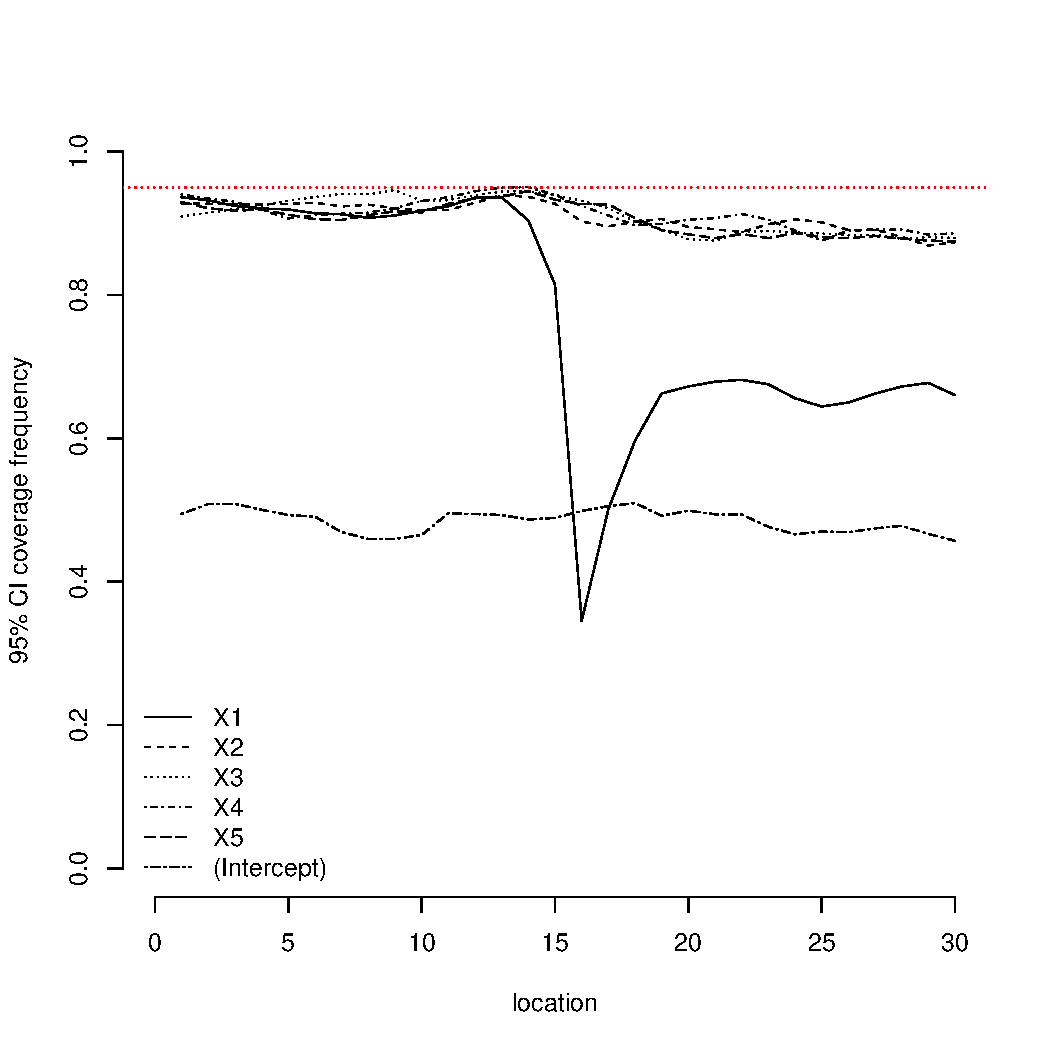
\includegraphics[width=\textwidth]{../../figures/simulation/15.9.profile_se_coverage.pdf}
		\caption{SE CI coverage}
		%\label{fig:gull}
	\end{subfigure}%
	\\%add desired spacing between images, e. g. ~, \quad, \qquad etc. 
          %(or a blank line to force the subfigure onto a new line)
	\begin{subfigure}[b]{0.45\textwidth}
	\centering
		\includegraphics[width=\textwidth]{../../figures/simulation/15.9.profile_unshrunk_bootstrap_coverage.pdf}
		\caption{Unshrunk bootstrap CI coverage}
		%\label{fig:gull}
	\end{subfigure}%
	~ %add desired spacing between images, e. g. ~, \quad, \qquad etc. 
	%(or a blank line to force the subfigure onto a new line)
	\begin{subfigure}[b]{0.45\textwidth}
	\centering
		\includegraphics[width=\textwidth]{../../figures/simulation/15.9.profile_selection.pdf}
		\caption{Selection frequency}
		%\label{fig:gull}
	\end{subfigure}
	\begin{subfigure}[b]{0.45\textwidth}
	\centering
		\includegraphics[width=\textwidth]{../../figures/simulation/X1.15.9.unshrunk_bootstrap_coverage.pdf}
		\caption{Unshrunk bootstrap CI coverage}
		%\label{fig:gull}
	\end{subfigure}%
	~ %add desired spacing between images, e. g. ~, \quad, \qquad etc. 
	%(or a blank line to force the subfigure onto a new line)
	\begin{subfigure}[b]{0.45\textwidth}
	\centering
		\includegraphics[width=\textwidth]{../../figures/simulation/X1.15.9.selection.pdf}
		\caption{Selection frequency}
		%\label{fig:gull}
	\end{subfigure}
	\caption{Simulation setting 9}
\end{figure}

\clearpage

\begin{figure}
	\vspace{-30mm}
	\centering
	\begin{subfigure}[b]{0.45\textwidth}
	\centering
		\includegraphics[width=\textwidth]{../../figures/simulation/15.10.profile_bootstrap_coverage.pdf}
		\caption{Bootstrap CI coverage}
		%\label{fig:gull}
	\end{subfigure}%
	~ %add desired spacing between images, e. g. ~, \quad, \qquad etc. 
	%(or a blank line to force the subfigure onto a new line)
	\begin{subfigure}[b]{0.45\textwidth}
	\centering
		\includegraphics[width=\textwidth]{../../figures/simulation/15.10.profile_se_coverage.pdf}
		\caption{SE CI coverage}
		%\label{fig:gull}
	\end{subfigure}%
	\\%add desired spacing between images, e. g. ~, \quad, \qquad etc. 
          %(or a blank line to force the subfigure onto a new line)
	\begin{subfigure}[b]{0.45\textwidth}
	\centering
		\includegraphics[width=\textwidth]{../../figures/simulation/15.10.profile_unshrunk_bootstrap_coverage.pdf}
		\caption{Unshrunk bootstrap CI coverage}
		%\label{fig:gull}
	\end{subfigure}%
	~ %add desired spacing between images, e. g. ~, \quad, \qquad etc. 
	%(or a blank line to force the subfigure onto a new line)
	\begin{subfigure}[b]{0.45\textwidth}
	\centering
		\includegraphics[width=\textwidth]{../../figures/simulation/15.10.profile_selection.pdf}
		\caption{Selection frequency}
		%\label{fig:gull}
	\end{subfigure}
	\begin{subfigure}[b]{0.45\textwidth}
	\centering
		\includegraphics[width=\textwidth]{../../figures/simulation/X1.15.10.unshrunk_bootstrap_coverage.pdf}
		\caption{Unshrunk bootstrap CI coverage}
		%\label{fig:gull}
	\end{subfigure}%
	~ %add desired spacing between images, e. g. ~, \quad, \qquad etc. 
	%(or a blank line to force the subfigure onto a new line)
	\begin{subfigure}[b]{0.45\textwidth}
	\centering
		\includegraphics[width=\textwidth]{../../figures/simulation/X1.15.10.selection.pdf}
		\caption{Selection frequency}
		%\label{fig:gull}
	\end{subfigure}
	\caption{Simulation setting 10}
\end{figure}
	
	\clearpage

\begin{figure}
	\vspace{-30mm}
	\centering
	\begin{subfigure}[b]{0.45\textwidth}
	\centering
		\includegraphics[width=\textwidth]{../../figures/simulation/15.11.profile_bootstrap_coverage.pdf}
		\caption{Bootstrap CI coverage}
		%\label{fig:gull}
	\end{subfigure}%
	~ %add desired spacing between images, e. g. ~, \quad, \qquad etc. 
	%(or a blank line to force the subfigure onto a new line)
	\begin{subfigure}[b]{0.45\textwidth}
	\centering
		\includegraphics[width=\textwidth]{../../figures/simulation/15.11.profile_se_coverage.pdf}
		\caption{SE CI coverage}
		%\label{fig:gull}
	\end{subfigure}%
	\\%add desired spacing between images, e. g. ~, \quad, \qquad etc. 
          %(or a blank line to force the subfigure onto a new line)
	\begin{subfigure}[b]{0.45\textwidth}
	\centering
		\includegraphics[width=\textwidth]{../../figures/simulation/15.11.profile_unshrunk_bootstrap_coverage.pdf}
		\caption{Unshrunk bootstrap CI coverage}
		%\label{fig:gull}
	\end{subfigure}%
	~ %add desired spacing between images, e. g. ~, \quad, \qquad etc. 
	%(or a blank line to force the subfigure onto a new line)
	\begin{subfigure}[b]{0.45\textwidth}
	\centering
		\includegraphics[width=\textwidth]{../../figures/simulation/15.11.profile_selection.pdf}
		\caption{Selection frequency}
		%\label{fig:gull}
	\end{subfigure}
	\begin{subfigure}[b]{0.45\textwidth}
	\centering
		\includegraphics[width=\textwidth]{../../figures/simulation/X1.15.11.unshrunk_bootstrap_coverage.pdf}
		\caption{Unshrunk bootstrap CI coverage}
		%\label{fig:gull}
	\end{subfigure}%
	~ %add desired spacing between images, e. g. ~, \quad, \qquad etc. 
	%(or a blank line to force the subfigure onto a new line)
	\begin{subfigure}[b]{0.45\textwidth}
	\centering
		\includegraphics[width=\textwidth]{../../figures/simulation/X1.15.11.selection.pdf}
		\caption{Selection frequency}
		%\label{fig:gull}
	\end{subfigure}
	\caption{Simulation setting 11}
\end{figure}

\clearpage

\begin{figure}
	\vspace{-30mm}
	\centering
	\begin{subfigure}[b]{0.45\textwidth}
	\centering
		\includegraphics[width=\textwidth]{../../figures/simulation/15.12.profile_bootstrap_coverage.pdf}
		\caption{Bootstrap CI coverage}
		%\label{fig:gull}
	\end{subfigure}%
	~ %add desired spacing between images, e. g. ~, \quad, \qquad etc. 
	%(or a blank line to force the subfigure onto a new line)
	\begin{subfigure}[b]{0.45\textwidth}
	\centering
		\includegraphics[width=\textwidth]{../../figures/simulation/15.12.profile_se_coverage.pdf}
		\caption{SE CI coverage}
		%\label{fig:gull}
	\end{subfigure}%
	\\%add desired spacing between images, e. g. ~, \quad, \qquad etc. 
          %(or a blank line to force the subfigure onto a new line)
	\begin{subfigure}[b]{0.45\textwidth}
	\centering
		\includegraphics[width=\textwidth]{../../figures/simulation/15.12.profile_unshrunk_bootstrap_coverage.pdf}
		\caption{Unshrunk bootstrap CI coverage}
		%\label{fig:gull}
	\end{subfigure}%
	~ %add desired spacing between images, e. g. ~, \quad, \qquad etc. 
	%(or a blank line to force the subfigure onto a new line)
	\begin{subfigure}[b]{0.45\textwidth}
	\centering
		\includegraphics[width=\textwidth]{../../figures/simulation/15.12.profile_selection.pdf}
		\caption{Selection frequency}
		%\label{fig:gull}
	\end{subfigure}
	\begin{subfigure}[b]{0.45\textwidth}
	\centering
		\includegraphics[width=\textwidth]{../../figures/simulation/X1.15.12.unshrunk_bootstrap_coverage.pdf}
		\caption{Unshrunk bootstrap CI coverage}
		%\label{fig:gull}
	\end{subfigure}%
	~ %add desired spacing between images, e. g. ~, \quad, \qquad etc. 
	%(or a blank line to force the subfigure onto a new line)
	\begin{subfigure}[b]{0.45\textwidth}
	\centering
		\includegraphics[width=\textwidth]{../../figures/simulation/X1.15.12.selection.pdf}
		\caption{Selection frequency}
		%\label{fig:gull}
	\end{subfigure}
	\caption{Simulation setting 12}
\end{figure}


\begin{figure}
	\vspace{-30mm}
	\centering
	\begin{subfigure}[b]{0.45\textwidth}
	\centering
		\includegraphics[width=\textwidth]{../../figures/simulation/15.13.profile_bootstrap_coverage.pdf}
		\caption{Bootstrap CI coverage}
		%\label{fig:gull}
	\end{subfigure}%
	~ %add desired spacing between images, e. g. ~, \quad, \qquad etc. 
	%(or a blank line to force the subfigure onto a new line)
	\begin{subfigure}[b]{0.45\textwidth}
	\centering
		\includegraphics[width=\textwidth]{../../figures/simulation/15.13.profile_se_coverage.pdf}
		\caption{SE CI coverage}
		%\label{fig:gull}
	\end{subfigure}%
	\\%add desired spacing between images, e. g. ~, \quad, \qquad etc. 
          %(or a blank line to force the subfigure onto a new line)
	\begin{subfigure}[b]{0.45\textwidth}
	\centering
		\includegraphics[width=\textwidth]{../../figures/simulation/15.13.profile_unshrunk_bootstrap_coverage.pdf}
		\caption{Unshrunk bootstrap CI coverage}
		%\label{fig:gull}
	\end{subfigure}%
	~ %add desired spacing between images, e. g. ~, \quad, \qquad etc. 
	%(or a blank line to force the subfigure onto a new line)
	\begin{subfigure}[b]{0.45\textwidth}
	\centering
		\includegraphics[width=\textwidth]{../../figures/simulation/15.13.profile_selection.pdf}
		\caption{Selection frequency}
		%\label{fig:gull}
	\end{subfigure}
	\begin{subfigure}[b]{0.45\textwidth}
	\centering
		\includegraphics[width=\textwidth]{../../figures/simulation/X1.15.13.unshrunk_bootstrap_coverage.pdf}
		\caption{Unshrunk bootstrap CI coverage}
		%\label{fig:gull}
	\end{subfigure}%
	~ %add desired spacing between images, e. g. ~, \quad, \qquad etc. 
	%(or a blank line to force the subfigure onto a new line)
	\begin{subfigure}[b]{0.45\textwidth}
	\centering
		\includegraphics[width=\textwidth]{../../figures/simulation/X1.15.13.selection.pdf}
		\caption{Selection frequency}
		%\label{fig:gull}
	\end{subfigure}
	\caption{Simulation setting 13}
\end{figure}


\begin{figure}
	\vspace{-30mm}
	\centering
	\begin{subfigure}[b]{0.45\textwidth}
	\centering
		\includegraphics[width=\textwidth]{../../figures/simulation/15.14.profile_bootstrap_coverage.pdf}
		\caption{Bootstrap CI coverage}
		%\label{fig:gull}
	\end{subfigure}%
	~ %add desired spacing between images, e. g. ~, \quad, \qquad etc. 
	%(or a blank line to force the subfigure onto a new line)
	\begin{subfigure}[b]{0.45\textwidth}
	\centering
		\includegraphics[width=\textwidth]{../../figures/simulation/15.14.profile_se_coverage.pdf}
		\caption{SE CI coverage}
		%\label{fig:gull}
	\end{subfigure}%
	\\%add desired spacing between images, e. g. ~, \quad, \qquad etc. 
          %(or a blank line to force the subfigure onto a new line)
	\begin{subfigure}[b]{0.45\textwidth}
	\centering
		\includegraphics[width=\textwidth]{../../figures/simulation/15.14.profile_unshrunk_bootstrap_coverage.pdf}
		\caption{Unshrunk bootstrap CI coverage}
		%\label{fig:gull}
	\end{subfigure}%
	~ %add desired spacing between images, e. g. ~, \quad, \qquad etc. 
	%(or a blank line to force the subfigure onto a new line)
	\begin{subfigure}[b]{0.45\textwidth}
	\centering
		\includegraphics[width=\textwidth]{../../figures/simulation/15.14.profile_selection.pdf}
		\caption{Selection frequency}
		%\label{fig:gull}
	\end{subfigure}
	\begin{subfigure}[b]{0.45\textwidth}
	\centering
		\includegraphics[width=\textwidth]{../../figures/simulation/X1.15.14.unshrunk_bootstrap_coverage.pdf}
		\caption{Unshrunk bootstrap CI coverage}
		%\label{fig:gull}
	\end{subfigure}%
	~ %add desired spacing between images, e. g. ~, \quad, \qquad etc. 
	%(or a blank line to force the subfigure onto a new line)
	\begin{subfigure}[b]{0.45\textwidth}
	\centering
		\includegraphics[width=\textwidth]{../../figures/simulation/X1.15.14.selection.pdf}
		\caption{Selection frequency}
		%\label{fig:gull}
	\end{subfigure}
	\caption{Simulation setting 14}
\end{figure}


\begin{figure}
	\vspace{-30mm}
	\centering
	\begin{subfigure}[b]{0.45\textwidth}
	\centering
		\includegraphics[width=\textwidth]{../../figures/simulation/15.15.profile_bootstrap_coverage.pdf}
		\caption{Bootstrap CI coverage}
		%\label{fig:gull}
	\end{subfigure}%
	~ %add desired spacing between images, e. g. ~, \quad, \qquad etc. 
	%(or a blank line to force the subfigure onto a new line)
	\begin{subfigure}[b]{0.45\textwidth}
	\centering
		\includegraphics[width=\textwidth]{../../figures/simulation/15.15.profile_se_coverage.pdf}
		\caption{SE CI coverage}
		%\label{fig:gull}
	\end{subfigure}%
	\\%add desired spacing between images, e. g. ~, \quad, \qquad etc. 
          %(or a blank line to force the subfigure onto a new line)
	\begin{subfigure}[b]{0.45\textwidth}
	\centering
		\includegraphics[width=\textwidth]{../../figures/simulation/15.15.profile_unshrunk_bootstrap_coverage.pdf}
		\caption{Unshrunk bootstrap CI coverage}
		%\label{fig:gull}
	\end{subfigure}%
	~ %add desired spacing between images, e. g. ~, \quad, \qquad etc. 
	%(or a blank line to force the subfigure onto a new line)
	\begin{subfigure}[b]{0.45\textwidth}
	\centering
		\includegraphics[width=\textwidth]{../../figures/simulation/15.15.profile_selection.pdf}
		\caption{Selection frequency}
		%\label{fig:gull}
	\end{subfigure}
	\begin{subfigure}[b]{0.45\textwidth}
	\centering
		\includegraphics[width=\textwidth]{../../figures/simulation/X1.15.15.unshrunk_bootstrap_coverage.pdf}
		\caption{Unshrunk bootstrap CI coverage}
		%\label{fig:gull}
	\end{subfigure}%
	~ %add desired spacing between images, e. g. ~, \quad, \qquad etc. 
	%(or a blank line to force the subfigure onto a new line)
	\begin{subfigure}[b]{0.45\textwidth}
	\centering
		\includegraphics[width=\textwidth]{../../figures/simulation/X1.15.15.selection.pdf}
		\caption{Selection frequency}
		%\label{fig:gull}
	\end{subfigure}
	\caption{Simulation setting 15}
\end{figure}


\begin{figure}
	\vspace{-30mm}
	\centering
	\begin{subfigure}[b]{0.45\textwidth}
	\centering
		\includegraphics[width=\textwidth]{../../figures/simulation/15.16.profile_bootstrap_coverage.pdf}
		\caption{Bootstrap CI coverage}
		%\label{fig:gull}
	\end{subfigure}%
	~ %add desired spacing between images, e. g. ~, \quad, \qquad etc. 
	%(or a blank line to force the subfigure onto a new line)
	\begin{subfigure}[b]{0.45\textwidth}
	\centering
		\includegraphics[width=\textwidth]{../../figures/simulation/15.16.profile_se_coverage.pdf}
		\caption{SE CI coverage}
		%\label{fig:gull}
	\end{subfigure}%
	\\%add desired spacing between images, e. g. ~, \quad, \qquad etc. 
          %(or a blank line to force the subfigure onto a new line)
	\begin{subfigure}[b]{0.45\textwidth}
	\centering
		\includegraphics[width=\textwidth]{../../figures/simulation/15.16.profile_unshrunk_bootstrap_coverage.pdf}
		\caption{Unshrunk bootstrap CI coverage}
		%\label{fig:gull}
	\end{subfigure}%
	~ %add desired spacing between images, e. g. ~, \quad, \qquad etc. 
	%(or a blank line to force the subfigure onto a new line)
	\begin{subfigure}[b]{0.45\textwidth}
	\centering
		\includegraphics[width=\textwidth]{../../figures/simulation/15.16.profile_selection.pdf}
		\caption{Selection frequency}
		%\label{fig:gull}
	\end{subfigure}
	\begin{subfigure}[b]{0.45\textwidth}
	\centering
		\includegraphics[width=\textwidth]{../../figures/simulation/X1.15.16.unshrunk_bootstrap_coverage.pdf}
		\caption{Unshrunk bootstrap CI coverage}
		%\label{fig:gull}
	\end{subfigure}%
	~ %add desired spacing between images, e. g. ~, \quad, \qquad etc. 
	%(or a blank line to force the subfigure onto a new line)
	\begin{subfigure}[b]{0.45\textwidth}
	\centering
		\includegraphics[width=\textwidth]{../../figures/simulation/X1.15.16.selection.pdf}
		\caption{Selection frequency}
		%\label{fig:gull}
	\end{subfigure}
	\caption{Simulation setting 16}
\end{figure}


\begin{figure}
	\vspace{-30mm}
	\centering
	\begin{subfigure}[b]{0.45\textwidth}
	\centering
		\includegraphics[width=\textwidth]{../../figures/simulation/15.17.profile_bootstrap_coverage.pdf}
		\caption{Bootstrap CI coverage}
		%\label{fig:gull}
	\end{subfigure}%
	~ %add desired spacing between images, e. g. ~, \quad, \qquad etc. 
	%(or a blank line to force the subfigure onto a new line)
	\begin{subfigure}[b]{0.45\textwidth}
	\centering
		\includegraphics[width=\textwidth]{../../figures/simulation/15.17.profile_se_coverage.pdf}
		\caption{SE CI coverage}
		%\label{fig:gull}
	\end{subfigure}%
	\\%add desired spacing between images, e. g. ~, \quad, \qquad etc. 
          %(or a blank line to force the subfigure onto a new line)
	\begin{subfigure}[b]{0.45\textwidth}
	\centering
		\includegraphics[width=\textwidth]{../../figures/simulation/15.17.profile_unshrunk_bootstrap_coverage.pdf}
		\caption{Unshrunk bootstrap CI coverage}
		%\label{fig:gull}
	\end{subfigure}%
	~ %add desired spacing between images, e. g. ~, \quad, \qquad etc. 
	%(or a blank line to force the subfigure onto a new line)
	\begin{subfigure}[b]{0.45\textwidth}
	\centering
		\includegraphics[width=\textwidth]{../../figures/simulation/15.17.profile_selection.pdf}
		\caption{Selection frequency}
		%\label{fig:gull}
	\end{subfigure}
	\begin{subfigure}[b]{0.45\textwidth}
	\centering
		\includegraphics[width=\textwidth]{../../figures/simulation/X1.15.17.unshrunk_bootstrap_coverage.pdf}
		\caption{Unshrunk bootstrap CI coverage}
		%\label{fig:gull}
	\end{subfigure}%
	~ %add desired spacing between images, e. g. ~, \quad, \qquad etc. 
	%(or a blank line to force the subfigure onto a new line)
	\begin{subfigure}[b]{0.45\textwidth}
	\centering
		\includegraphics[width=\textwidth]{../../figures/simulation/X1.15.17.selection.pdf}
		\caption{Selection frequency}
		%\label{fig:gull}
	\end{subfigure}
	\caption{Simulation setting 17}
\end{figure}


\begin{figure}
	\vspace{-30mm}
	\centering
	\begin{subfigure}[b]{0.45\textwidth}
	\centering
		\includegraphics[width=\textwidth]{../../figures/simulation/15.18.profile_bootstrap_coverage.pdf}
		\caption{Bootstrap CI coverage}
		%\label{fig:gull}
	\end{subfigure}%
	~ %add desired spacing between images, e. g. ~, \quad, \qquad etc. 
	%(or a blank line to force the subfigure onto a new line)
	\begin{subfigure}[b]{0.45\textwidth}
	\centering
		\includegraphics[width=\textwidth]{../../figures/simulation/15.18.profile_se_coverage.pdf}
		\caption{SE CI coverage}
		%\label{fig:gull}
	\end{subfigure}%
	\\%add desired spacing between images, e. g. ~, \quad, \qquad etc. 
          %(or a blank line to force the subfigure onto a new line)
	\begin{subfigure}[b]{0.45\textwidth}
	\centering
		\includegraphics[width=\textwidth]{../../figures/simulation/15.18.profile_unshrunk_bootstrap_coverage.pdf}
		\caption{Unshrunk bootstrap CI coverage}
		%\label{fig:gull}
	\end{subfigure}%
	~ %add desired spacing between images, e. g. ~, \quad, \qquad etc. 
	%(or a blank line to force the subfigure onto a new line)
	\begin{subfigure}[b]{0.45\textwidth}
	\centering
		\includegraphics[width=\textwidth]{../../figures/simulation/15.18.profile_selection.pdf}
		\caption{Selection frequency}
		%\label{fig:gull}
	\end{subfigure}
	\begin{subfigure}[b]{0.45\textwidth}
	\centering
		\includegraphics[width=\textwidth]{../../figures/simulation/X1.15.18.unshrunk_bootstrap_coverage.pdf}
		\caption{Unshrunk bootstrap CI coverage}
		%\label{fig:gull}
	\end{subfigure}%
	~ %add desired spacing between images, e. g. ~, \quad, \qquad etc. 
	%(or a blank line to force the subfigure onto a new line)
	\begin{subfigure}[b]{0.45\textwidth}
	\centering
		\includegraphics[width=\textwidth]{../../figures/simulation/X1.15.18.selection.pdf}
		\caption{Selection frequency}
		%\label{fig:gull}
	\end{subfigure}
	\caption{Simulation setting 18}
\end{figure}


\begin{figure}
	\vspace{-30mm}
	\centering
	\begin{subfigure}[b]{0.45\textwidth}
	\centering
		\includegraphics[width=\textwidth]{../../figures/simulation/15.19.profile_bootstrap_coverage.pdf}
		\caption{Bootstrap CI coverage}
		%\label{fig:gull}
	\end{subfigure}%
	~ %add desired spacing between images, e. g. ~, \quad, \qquad etc. 
	%(or a blank line to force the subfigure onto a new line)
	\begin{subfigure}[b]{0.45\textwidth}
	\centering
		\includegraphics[width=\textwidth]{../../figures/simulation/15.19.profile_se_coverage.pdf}
		\caption{SE CI coverage}
		%\label{fig:gull}
	\end{subfigure}%
	\\%add desired spacing between images, e. g. ~, \quad, \qquad etc. 
          %(or a blank line to force the subfigure onto a new line)
	\begin{subfigure}[b]{0.45\textwidth}
	\centering
		\includegraphics[width=\textwidth]{../../figures/simulation/15.19.profile_unshrunk_bootstrap_coverage.pdf}
		\caption{Unshrunk bootstrap CI coverage}
		%\label{fig:gull}
	\end{subfigure}%
	~ %add desired spacing between images, e. g. ~, \quad, \qquad etc. 
	%(or a blank line to force the subfigure onto a new line)
	\begin{subfigure}[b]{0.45\textwidth}
	\centering
		\includegraphics[width=\textwidth]{../../figures/simulation/15.19.profile_selection.pdf}
		\caption{Selection frequency}
		%\label{fig:gull}
	\end{subfigure}
	\begin{subfigure}[b]{0.45\textwidth}
	\centering
		\includegraphics[width=\textwidth]{../../figures/simulation/X1.15.19.unshrunk_bootstrap_coverage.pdf}
		\caption{Unshrunk bootstrap CI coverage}
		%\label{fig:gull}
	\end{subfigure}%
	~ %add desired spacing between images, e. g. ~, \quad, \qquad etc. 
	%(or a blank line to force the subfigure onto a new line)
	\begin{subfigure}[b]{0.45\textwidth}
	\centering
		\includegraphics[width=\textwidth]{../../figures/simulation/X1.15.19.selection.pdf}
		\caption{Selection frequency}
		%\label{fig:gull}
	\end{subfigure}
	\caption{Simulation setting 19}
\end{figure}


\begin{figure}
	\vspace{-30mm}
	\centering
	\begin{subfigure}[b]{0.45\textwidth}
	\centering
		\includegraphics[width=\textwidth]{../../figures/simulation/15.20.profile_bootstrap_coverage.pdf}
		\caption{Bootstrap CI coverage}
		%\label{fig:gull}
	\end{subfigure}%
	~ %add desired spacing between images, e. g. ~, \quad, \qquad etc. 
	%(or a blank line to force the subfigure onto a new line)
	\begin{subfigure}[b]{0.45\textwidth}
	\centering
		\includegraphics[width=\textwidth]{../../figures/simulation/15.20.profile_se_coverage.pdf}
		\caption{SE CI coverage}
		%\label{fig:gull}
	\end{subfigure}%
	\\%add desired spacing between images, e. g. ~, \quad, \qquad etc. 
          %(or a blank line to force the subfigure onto a new line)
	\begin{subfigure}[b]{0.45\textwidth}
	\centering
		\includegraphics[width=\textwidth]{../../figures/simulation/15.20.profile_unshrunk_bootstrap_coverage.pdf}
		\caption{Unshrunk bootstrap CI coverage}
		%\label{fig:gull}
	\end{subfigure}%
	~ %add desired spacing between images, e. g. ~, \quad, \qquad etc. 
	%(or a blank line to force the subfigure onto a new line)
	\begin{subfigure}[b]{0.45\textwidth}
	\centering
		\includegraphics[width=\textwidth]{../../figures/simulation/15.20.profile_selection.pdf}
		\caption{Selection frequency}
		%\label{fig:gull}
	\end{subfigure}
	\begin{subfigure}[b]{0.45\textwidth}
	\centering
		\includegraphics[width=\textwidth]{../../figures/simulation/X1.15.20.unshrunk_bootstrap_coverage.pdf}
		\caption{Unshrunk bootstrap CI coverage}
		%\label{fig:gull}
	\end{subfigure}%
	~ %add desired spacing between images, e. g. ~, \quad, \qquad etc. 
	%(or a blank line to force the subfigure onto a new line)
	\begin{subfigure}[b]{0.45\textwidth}
	\centering
		\includegraphics[width=\textwidth]{../../figures/simulation/X1.15.20.selection.pdf}
		\caption{Selection frequency}
		%\label{fig:gull}
	\end{subfigure}
	\caption{Simulation setting 20}
\end{figure}


\begin{figure}
	\vspace{-30mm}
	\centering
	\begin{subfigure}[b]{0.45\textwidth}
	\centering
		\includegraphics[width=\textwidth]{../../figures/simulation/15.21.profile_bootstrap_coverage.pdf}
		\caption{Bootstrap CI coverage}
		%\label{fig:gull}
	\end{subfigure}%
	~ %add desired spacing between images, e. g. ~, \quad, \qquad etc. 
	%(or a blank line to force the subfigure onto a new line)
	\begin{subfigure}[b]{0.45\textwidth}
	\centering
		\includegraphics[width=\textwidth]{../../figures/simulation/15.21.profile_se_coverage.pdf}
		\caption{SE CI coverage}
		%\label{fig:gull}
	\end{subfigure}%
	\\%add desired spacing between images, e. g. ~, \quad, \qquad etc. 
          %(or a blank line to force the subfigure onto a new line)
	\begin{subfigure}[b]{0.45\textwidth}
	\centering
		\includegraphics[width=\textwidth]{../../figures/simulation/15.21.profile_unshrunk_bootstrap_coverage.pdf}
		\caption{Unshrunk bootstrap CI coverage}
		%\label{fig:gull}
	\end{subfigure}%
	~ %add desired spacing between images, e. g. ~, \quad, \qquad etc. 
	%(or a blank line to force the subfigure onto a new line)
	\begin{subfigure}[b]{0.45\textwidth}
	\centering
		\includegraphics[width=\textwidth]{../../figures/simulation/15.21.profile_selection.pdf}
		\caption{Selection frequency}
		%\label{fig:gull}
	\end{subfigure}
	\begin{subfigure}[b]{0.45\textwidth}
	\centering
		\includegraphics[width=\textwidth]{../../figures/simulation/X1.15.21.unshrunk_bootstrap_coverage.pdf}
		\caption{Unshrunk bootstrap CI coverage}
		%\label{fig:gull}
	\end{subfigure}%
	~ %add desired spacing between images, e. g. ~, \quad, \qquad etc. 
	%(or a blank line to force the subfigure onto a new line)
	\begin{subfigure}[b]{0.45\textwidth}
	\centering
		\includegraphics[width=\textwidth]{../../figures/simulation/X1.15.21.selection.pdf}
		\caption{Selection frequency}
		%\label{fig:gull}
	\end{subfigure}
	\caption{Simulation setting 21}
\end{figure}


\begin{figure}
	\vspace{-30mm}
	\centering
	\begin{subfigure}[b]{0.45\textwidth}
	\centering
		\includegraphics[width=\textwidth]{../../figures/simulation/15.22.profile_bootstrap_coverage.pdf}
		\caption{Bootstrap CI coverage}
		%\label{fig:gull}
	\end{subfigure}%
	~ %add desired spacing between images, e. g. ~, \quad, \qquad etc. 
	%(or a blank line to force the subfigure onto a new line)
	\begin{subfigure}[b]{0.45\textwidth}
	\centering
		\includegraphics[width=\textwidth]{../../figures/simulation/15.22.profile_se_coverage.pdf}
		\caption{SE CI coverage}
		%\label{fig:gull}
	\end{subfigure}%
	\\%add desired spacing between images, e. g. ~, \quad, \qquad etc. 
          %(or a blank line to force the subfigure onto a new line)
	\begin{subfigure}[b]{0.45\textwidth}
	\centering
		\includegraphics[width=\textwidth]{../../figures/simulation/15.22.profile_unshrunk_bootstrap_coverage.pdf}
		\caption{Unshrunk bootstrap CI coverage}
		%\label{fig:gull}
	\end{subfigure}%
	~ %add desired spacing between images, e. g. ~, \quad, \qquad etc. 
	%(or a blank line to force the subfigure onto a new line)
	\begin{subfigure}[b]{0.45\textwidth}
	\centering
		\includegraphics[width=\textwidth]{../../figures/simulation/15.22.profile_selection.pdf}
		\caption{Selection frequency}
		%\label{fig:gull}
	\end{subfigure}
	\begin{subfigure}[b]{0.45\textwidth}
	\centering
		\includegraphics[width=\textwidth]{../../figures/simulation/X1.15.22.unshrunk_bootstrap_coverage.pdf}
		\caption{Unshrunk bootstrap CI coverage}
		%\label{fig:gull}
	\end{subfigure}%
	~ %add desired spacing between images, e. g. ~, \quad, \qquad etc. 
	%(or a blank line to force the subfigure onto a new line)
	\begin{subfigure}[b]{0.45\textwidth}
	\centering
		\includegraphics[width=\textwidth]{../../figures/simulation/X1.15.22.selection.pdf}
		\caption{Selection frequency}
		%\label{fig:gull}
	\end{subfigure}
	\caption{Simulation setting 22}
\end{figure}


\begin{figure}
	\vspace{-30mm}
	\centering
	\begin{subfigure}[b]{0.45\textwidth}
	\centering
		\includegraphics[width=\textwidth]{../../figures/simulation/15.23.profile_bootstrap_coverage.pdf}
		\caption{Bootstrap CI coverage}
		%\label{fig:gull}
	\end{subfigure}%
	~ %add desired spacing between images, e. g. ~, \quad, \qquad etc. 
	%(or a blank line to force the subfigure onto a new line)
	\begin{subfigure}[b]{0.45\textwidth}
	\centering
		\includegraphics[width=\textwidth]{../../figures/simulation/15.23.profile_se_coverage.pdf}
		\caption{SE CI coverage}
		%\label{fig:gull}
	\end{subfigure}%
	\\%add desired spacing between images, e. g. ~, \quad, \qquad etc. 
          %(or a blank line to force the subfigure onto a new line)
	\begin{subfigure}[b]{0.45\textwidth}
	\centering
		\includegraphics[width=\textwidth]{../../figures/simulation/15.23.profile_unshrunk_bootstrap_coverage.pdf}
		\caption{Unshrunk bootstrap CI coverage}
		%\label{fig:gull}
	\end{subfigure}%
	~ %add desired spacing between images, e. g. ~, \quad, \qquad etc. 
	%(or a blank line to force the subfigure onto a new line)
	\begin{subfigure}[b]{0.45\textwidth}
	\centering
		\includegraphics[width=\textwidth]{../../figures/simulation/15.23.profile_selection.pdf}
		\caption{Selection frequency}
		%\label{fig:gull}
	\end{subfigure}
	\begin{subfigure}[b]{0.45\textwidth}
	\centering
		\includegraphics[width=\textwidth]{../../figures/simulation/X1.15.23.unshrunk_bootstrap_coverage.pdf}
		\caption{Unshrunk bootstrap CI coverage}
		%\label{fig:gull}
	\end{subfigure}%
	~ %add desired spacing between images, e. g. ~, \quad, \qquad etc. 
	%(or a blank line to force the subfigure onto a new line)
	\begin{subfigure}[b]{0.45\textwidth}
	\centering
		\includegraphics[width=\textwidth]{../../figures/simulation/X1.15.23.selection.pdf}
		\caption{Selection frequency}
		%\label{fig:gull}
	\end{subfigure}
	\caption{Simulation setting 23}
\end{figure}


\begin{figure}
	\vspace{-30mm}
	\centering
	\begin{subfigure}[b]{0.45\textwidth}
	\centering
		\includegraphics[width=\textwidth]{../../figures/simulation/15.24.profile_bootstrap_coverage.pdf}
		\caption{Bootstrap CI coverage}
		%\label{fig:gull}
	\end{subfigure}%
	~ %add desired spacing between images, e. g. ~, \quad, \qquad etc. 
	%(or a blank line to force the subfigure onto a new line)
	\begin{subfigure}[b]{0.45\textwidth}
	\centering
		\includegraphics[width=\textwidth]{../../figures/simulation/15.24.profile_se_coverage.pdf}
		\caption{SE CI coverage}
		%\label{fig:gull}
	\end{subfigure}%
	\\%add desired spacing between images, e. g. ~, \quad, \qquad etc. 
          %(or a blank line to force the subfigure onto a new line)
	\begin{subfigure}[b]{0.45\textwidth}
	\centering
		\includegraphics[width=\textwidth]{../../figures/simulation/15.24.profile_unshrunk_bootstrap_coverage.pdf}
		\caption{Unshrunk bootstrap CI coverage}
		%\label{fig:gull}
	\end{subfigure}%
	~ %add desired spacing between images, e. g. ~, \quad, \qquad etc. 
	%(or a blank line to force the subfigure onto a new line)
	\begin{subfigure}[b]{0.45\textwidth}
	\centering
		\includegraphics[width=\textwidth]{../../figures/simulation/15.24.profile_selection.pdf}
		\caption{Selection frequency}
		%\label{fig:gull}
	\end{subfigure}
	\begin{subfigure}[b]{0.45\textwidth}
	\centering
		\includegraphics[width=\textwidth]{../../figures/simulation/X1.15.24.unshrunk_bootstrap_coverage.pdf}
		\caption{Unshrunk bootstrap CI coverage}
		%\label{fig:gull}
	\end{subfigure}%
	~ %add desired spacing between images, e. g. ~, \quad, \qquad etc. 
	%(or a blank line to force the subfigure onto a new line)
	\begin{subfigure}[b]{0.45\textwidth}
	\centering
		\includegraphics[width=\textwidth]{../../figures/simulation/X1.15.24.selection.pdf}
		\caption{Selection frequency}
		%\label{fig:gull}
	\end{subfigure}
	\caption{Simulation setting 24}
\end{figure}


\begin{figure}
	\vspace{-30mm}
	\centering
	\begin{subfigure}[b]{0.45\textwidth}
	\centering
		\includegraphics[width=\textwidth]{../../figures/simulation/15.25.profile_bootstrap_coverage.pdf}
		\caption{Bootstrap CI coverage}
		%\label{fig:gull}
	\end{subfigure}%
	~ %add desired spacing between images, e. g. ~, \quad, \qquad etc. 
	%(or a blank line to force the subfigure onto a new line)
	\begin{subfigure}[b]{0.45\textwidth}
	\centering
		\includegraphics[width=\textwidth]{../../figures/simulation/15.25.profile_se_coverage.pdf}
		\caption{SE CI coverage}
		%\label{fig:gull}
	\end{subfigure}%
	\\%add desired spacing between images, e. g. ~, \quad, \qquad etc. 
          %(or a blank line to force the subfigure onto a new line)
	\begin{subfigure}[b]{0.45\textwidth}
	\centering
		\includegraphics[width=\textwidth]{../../figures/simulation/15.25.profile_unshrunk_bootstrap_coverage.pdf}
		\caption{Unshrunk bootstrap CI coverage}
		%\label{fig:gull}
	\end{subfigure}%
	~ %add desired spacing between images, e. g. ~, \quad, \qquad etc. 
	%(or a blank line to force the subfigure onto a new line)
	\begin{subfigure}[b]{0.45\textwidth}
	\centering
		\includegraphics[width=\textwidth]{../../figures/simulation/15.25.profile_selection.pdf}
		\caption{Selection frequency}
		%\label{fig:gull}
	\end{subfigure}
	\begin{subfigure}[b]{0.45\textwidth}
	\centering
		\includegraphics[width=\textwidth]{../../figures/simulation/X1.15.25.unshrunk_bootstrap_coverage.pdf}
		\caption{Unshrunk bootstrap CI coverage}
		%\label{fig:gull}
	\end{subfigure}%
	~ %add desired spacing between images, e. g. ~, \quad, \qquad etc. 
	%(or a blank line to force the subfigure onto a new line)
	\begin{subfigure}[b]{0.45\textwidth}
	\centering
		\includegraphics[width=\textwidth]{../../figures/simulation/X1.15.25.selection.pdf}
		\caption{Selection frequency}
		%\label{fig:gull}
	\end{subfigure}
	\caption{Simulation setting 25}
\end{figure}


\begin{figure}
	\vspace{-30mm}
	\centering
	\begin{subfigure}[b]{0.45\textwidth}
	\centering
		\includegraphics[width=\textwidth]{../../figures/simulation/15.26.profile_bootstrap_coverage.pdf}
		\caption{Bootstrap CI coverage}
		%\label{fig:gull}
	\end{subfigure}%
	~ %add desired spacing between images, e. g. ~, \quad, \qquad etc. 
	%(or a blank line to force the subfigure onto a new line)
	\begin{subfigure}[b]{0.45\textwidth}
	\centering
		\includegraphics[width=\textwidth]{../../figures/simulation/15.26.profile_se_coverage.pdf}
		\caption{SE CI coverage}
		%\label{fig:gull}
	\end{subfigure}%
	\\%add desired spacing between images, e. g. ~, \quad, \qquad etc. 
          %(or a blank line to force the subfigure onto a new line)
	\begin{subfigure}[b]{0.45\textwidth}
	\centering
		\includegraphics[width=\textwidth]{../../figures/simulation/15.26.profile_unshrunk_bootstrap_coverage.pdf}
		\caption{Unshrunk bootstrap CI coverage}
		%\label{fig:gull}
	\end{subfigure}%
	~ %add desired spacing between images, e. g. ~, \quad, \qquad etc. 
	%(or a blank line to force the subfigure onto a new line)
	\begin{subfigure}[b]{0.45\textwidth}
	\centering
		\includegraphics[width=\textwidth]{../../figures/simulation/15.26.profile_selection.pdf}
		\caption{Selection frequency}
		%\label{fig:gull}
	\end{subfigure}
	\begin{subfigure}[b]{0.45\textwidth}
	\centering
		\includegraphics[width=\textwidth]{../../figures/simulation/X1.15.26.unshrunk_bootstrap_coverage.pdf}
		\caption{Unshrunk bootstrap CI coverage}
		%\label{fig:gull}
	\end{subfigure}%
	~ %add desired spacing between images, e. g. ~, \quad, \qquad etc. 
	%(or a blank line to force the subfigure onto a new line)
	\begin{subfigure}[b]{0.45\textwidth}
	\centering
		\includegraphics[width=\textwidth]{../../figures/simulation/X1.15.26.selection.pdf}
		\caption{Selection frequency}
		%\label{fig:gull}
	\end{subfigure}
	\caption{Simulation setting 26}
\end{figure}

\clearpage

\begin{figure}
	\vspace{-30mm}
	\centering
	\begin{subfigure}[b]{0.45\textwidth}
	\centering
		\includegraphics[width=\textwidth]{../../figures/simulation/15.27.profile_bootstrap_coverage.pdf}
		\caption{Bootstrap CI coverage}
		%\label{fig:gull}
	\end{subfigure}%
	~ %add desired spacing between images, e. g. ~, \quad, \qquad etc. 
	%(or a blank line to force the subfigure onto a new line)
	\begin{subfigure}[b]{0.45\textwidth}
	\centering
		\includegraphics[width=\textwidth]{../../figures/simulation/15.27.profile_se_coverage.pdf}
		\caption{SE CI coverage}
		%\label{fig:gull}
	\end{subfigure}%
	\\%add desired spacing between images, e. g. ~, \quad, \qquad etc. 
          %(or a blank line to force the subfigure onto a new line)
	%\begin{subfigure}[b]{0.45\textwidth}
	%\centering
	%	\includegraphics[width=\textwidth]{../../figures/simulation/15.27.profile_unshrunk_bootstrap_coverage.pdf}
	%	\caption{Unshrunk bootstrap CI coverage}
	%	%\label{fig:gull}
	%\end{subfigure}%
	~ %add desired spacing between images, e. g. ~, \quad, \qquad etc. 
	%(or a blank line to force the subfigure onto a new line)
	\begin{subfigure}[b]{0.45\textwidth}
	\centering
		\includegraphics[width=\textwidth]{../../figures/simulation/15.27.profile_selection.pdf}
		\caption{Selection frequency}
		%\label{fig:gull}
	\end{subfigure}
	%\begin{subfigure}[b]{0.45\textwidth}
	%\centering
	%	\includegraphics[width=\textwidth]{../../figures/simulation/X1.15.27.unshrunk_bootstrap_coverage.pdf}
	%	\caption{Unshrunk bootstrap CI coverage}
	%	%\label{fig:gull}
	%\end{subfigure}%
	~ %add desired spacing between images, e. g. ~, \quad, \qquad etc. 
	%(or a blank line to force the subfigure onto a new line)
	\begin{subfigure}[b]{0.45\textwidth}
	\centering
		\includegraphics[width=\textwidth]{../../figures/simulation/X1.15.27.selection.pdf}
		\caption{Selection frequency}
		%\label{fig:gull}
	\end{subfigure}
	\caption{Simulation setting 27}
\end{figure}


\begin{figure}
	\vspace{-30mm}
	\centering
	\begin{subfigure}[b]{0.45\textwidth}
	\centering
		\includegraphics[width=\textwidth]{../../figures/simulation/15.28.profile_bootstrap_coverage.pdf}
		\caption{Bootstrap CI coverage}
		%\label{fig:gull}
	\end{subfigure}%
	~ %add desired spacing between images, e. g. ~, \quad, \qquad etc. 
	%(or a blank line to force the subfigure onto a new line)
	\begin{subfigure}[b]{0.45\textwidth}
	\centering
		\includegraphics[width=\textwidth]{../../figures/simulation/15.28.profile_se_coverage.pdf}
		\caption{SE CI coverage}
		%\label{fig:gull}
	\end{subfigure}%
	\\%add desired spacing between images, e. g. ~, \quad, \qquad etc. 
          %(or a blank line to force the subfigure onto a new line)
	%\begin{subfigure}[b]{0.45\textwidth}
	%\centering
	%	\includegraphics[width=\textwidth]{../../figures/simulation/15.28.profile_unshrunk_bootstrap_coverage.pdf}
	%	\caption{Unshrunk bootstrap CI coverage}
	%	%\label{fig:gull}
	%\end{subfigure}%
	~ %add desired spacing between images, e. g. ~, \quad, \qquad etc. 
	%(or a blank line to force the subfigure onto a new line)
	\begin{subfigure}[b]{0.45\textwidth}
	\centering
		\includegraphics[width=\textwidth]{../../figures/simulation/15.28.profile_selection.pdf}
		\caption{Selection frequency}
		%\label{fig:gull}
	\end{subfigure}
	%\begin{subfigure}[b]{0.45\textwidth}
	%\centering
	%	\includegraphics[width=\textwidth]{../../figures/simulation/X1.15.28.unshrunk_bootstrap_coverage.pdf}
	%	\caption{Unshrunk bootstrap CI coverage}
	%	%\label{fig:gull}
	%\end{subfigure}%
	~ %add desired spacing between images, e. g. ~, \quad, \qquad etc. 
	%(or a blank line to force the subfigure onto a new line)
	\begin{subfigure}[b]{0.45\textwidth}
	\centering
		\includegraphics[width=\textwidth]{../../figures/simulation/X1.15.28.selection.pdf}
		\caption{Selection frequency}
		%\label{fig:gull}
	\end{subfigure}
	\caption{Simulation setting 28}
\end{figure}

\clearpage

\begin{figure}
	\vspace{-30mm}
	\centering
	\begin{subfigure}[b]{0.45\textwidth}
	\centering
		\includegraphics[width=\textwidth]{../../figures/simulation/15.29.profile_bootstrap_coverage.pdf}
		\caption{Bootstrap CI coverage}
		%\label{fig:gull}
	\end{subfigure}%
	~ %add desired spacing between images, e. g. ~, \quad, \qquad etc. 
	%(or a blank line to force the subfigure onto a new line)
	\begin{subfigure}[b]{0.45\textwidth}
	\centering
		\includegraphics[width=\textwidth]{../../figures/simulation/15.29.profile_se_coverage.pdf}
		\caption{SE CI coverage}
		%\label{fig:gull}
	\end{subfigure}%
	\\%add desired spacing between images, e. g. ~, \quad, \qquad etc. 
          %(or a blank line to force the subfigure onto a new line)
	%\begin{subfigure}[b]{0.45\textwidth}
	%\centering
	%	\includegraphics[width=\textwidth]{../../figures/simulation/15.29.profile_unshrunk_bootstrap_coverage.pdf}
	%	\caption{Unshrunk bootstrap CI coverage}
	%	%\label{fig:gull}
	%\end{subfigure}%
	~ %add desired spacing between images, e. g. ~, \quad, \qquad etc. 
	%(or a blank line to force the subfigure onto a new line)
	\begin{subfigure}[b]{0.45\textwidth}
	\centering
		\includegraphics[width=\textwidth]{../../figures/simulation/15.29.profile_selection.pdf}
		\caption{Selection frequency}
		%\label{fig:gull}
	\end{subfigure}
	%\begin{subfigure}[b]{0.45\textwidth}
	%\centering
	%	\includegraphics[width=\textwidth]{../../figures/simulation/X1.15.29.unshrunk_bootstrap_coverage.pdf}
	%	\caption{Unshrunk bootstrap CI coverage}
	%	%\label{fig:gull}
	%\end{subfigure}%
	~ %add desired spacing between images, e. g. ~, \quad, \qquad etc. 
	%(or a blank line to force the subfigure onto a new line)
	\begin{subfigure}[b]{0.45\textwidth}
	\centering
		\includegraphics[width=\textwidth]{../../figures/simulation/X1.15.29.selection.pdf}
		\caption{Selection frequency}
		%\label{fig:gull}
	\end{subfigure}
	\caption{Simulation setting 29}
\end{figure}


\begin{figure}
	\vspace{-30mm}
	\centering
	\begin{subfigure}[b]{0.45\textwidth}
	\centering
		\includegraphics[width=\textwidth]{../../figures/simulation/15.30.profile_bootstrap_coverage.pdf}
		\caption{Bootstrap CI coverage}
		%\label{fig:gull}
	\end{subfigure}%
	~ %add desired spacing between images, e. g. ~, \quad, \qquad etc. 
	%(or a blank line to force the subfigure onto a new line)
	\begin{subfigure}[b]{0.45\textwidth}
	\centering
		\includegraphics[width=\textwidth]{../../figures/simulation/15.30.profile_se_coverage.pdf}
		\caption{SE CI coverage}
		%\label{fig:gull}
	\end{subfigure}%
	\\%add desired spacing between images, e. g. ~, \quad, \qquad etc. 
          %(or a blank line to force the subfigure onto a new line)
	%\begin{subfigure}[b]{0.45\textwidth}
	%\centering
	%	\includegraphics[width=\textwidth]{../../figures/simulation/15.30.profile_unshrunk_bootstrap_coverage.pdf}
	%	\caption{Unshrunk bootstrap CI coverage}
	%	%\label{fig:gull}
	%\end{subfigure}%
	~ %add desired spacing between images, e. g. ~, \quad, \qquad etc. 
	%(or a blank line to force the subfigure onto a new line)
	\begin{subfigure}[b]{0.45\textwidth}
	\centering
		\includegraphics[width=\textwidth]{../../figures/simulation/15.30.profile_selection.pdf}
		\caption{Selection frequency}
		%\label{fig:gull}
	\end{subfigure}
	%\begin{subfigure}[b]{0.45\textwidth}
	%\centering
	%	\includegraphics[width=\textwidth]{../../figures/simulation/X1.15.30.unshrunk_bootstrap_coverage.pdf}
	%	\caption{Unshrunk bootstrap CI coverage}
	%	%\label{fig:gull}
	%\end{subfigure}%
	~ %add desired spacing between images, e. g. ~, \quad, \qquad etc. 
	%(or a blank line to force the subfigure onto a new line)
	\begin{subfigure}[b]{0.45\textwidth}
	\centering
		\includegraphics[width=\textwidth]{../../figures/simulation/X1.15.30.selection.pdf}
		\caption{Selection frequency}
		%\label{fig:gull}
	\end{subfigure}
	\caption{Simulation setting 30}
\end{figure}



\begin{figure}
	\vspace{-30mm}
	\centering
	\begin{subfigure}[b]{0.45\textwidth}
	\centering
		\includegraphics[width=\textwidth]{../../figures/simulation/15.31.profile_bootstrap_coverage.pdf}
		\caption{Bootstrap CI coverage}
		%\label{fig:gull}
	\end{subfigure}%
	~ %add desired spacing between images, e. g. ~, \quad, \qquad etc. 
	%(or a blank line to force the subfigure onto a new line)
	\begin{subfigure}[b]{0.45\textwidth}
	\centering
		\includegraphics[width=\textwidth]{../../figures/simulation/15.31.profile_se_coverage.pdf}
		\caption{SE CI coverage}
		%\label{fig:gull}
	\end{subfigure}%
	\\%add desired spacing between images, e. g. ~, \quad, \qquad etc. 
          %(or a blank line to force the subfigure onto a new line)
	%\begin{subfigure}[b]{0.45\textwidth}
	%\centering
	%	\includegraphics[width=\textwidth]{../../figures/simulation/15.31.profile_unshrunk_bootstrap_coverage.pdf}
	%	\caption{Unshrunk bootstrap CI coverage}
	%	%\label{fig:gull}
	%\end{subfigure}%
	~ %add desired spacing between images, e. g. ~, \quad, \qquad etc. 
	%(or a blank line to force the subfigure onto a new line)
	\begin{subfigure}[b]{0.45\textwidth}
	\centering
		\includegraphics[width=\textwidth]{../../figures/simulation/15.31.profile_selection.pdf}
		\caption{Selection frequency}
		%\label{fig:gull}
	\end{subfigure}
	%\begin{subfigure}[b]{0.45\textwidth}
	%\centering
	%	\includegraphics[width=\textwidth]{../../figures/simulation/X1.15.31.unshrunk_bootstrap_coverage.pdf}
	%	\caption{Unshrunk bootstrap CI coverage}
	%	%\label{fig:gull}
	%\end{subfigure}%
	~ %add desired spacing between images, e. g. ~, \quad, \qquad etc. 
	%(or a blank line to force the subfigure onto a new line)
	\begin{subfigure}[b]{0.45\textwidth}
	\centering
		\includegraphics[width=\textwidth]{../../figures/simulation/X1.15.31.selection.pdf}
		\caption{Selection frequency}
		%\label{fig:gull}
	\end{subfigure}
	\caption{Simulation setting 31}
\end{figure}

\clearpage

\begin{figure}
	\vspace{-30mm}
	\centering
	\begin{subfigure}[b]{0.45\textwidth}
	\centering
		\includegraphics[width=\textwidth]{../../figures/simulation/15.32.profile_bootstrap_coverage.pdf}
		\caption{Bootstrap CI coverage}
		%\label{fig:gull}
	\end{subfigure}%
	~ %add desired spacing between images, e. g. ~, \quad, \qquad etc. 
	%(or a blank line to force the subfigure onto a new line)
	\begin{subfigure}[b]{0.45\textwidth}
	\centering
		\includegraphics[width=\textwidth]{../../figures/simulation/15.32.profile_se_coverage.pdf}
		\caption{SE CI coverage}
		%\label{fig:gull}
	\end{subfigure}%
	\\%add desired spacing between images, e. g. ~, \quad, \qquad etc. 
          %(or a blank line to force the subfigure onto a new line)
	%\begin{subfigure}[b]{0.45\textwidth}
	%\centering
	%	\includegraphics[width=\textwidth]{../../figures/simulation/15.32.profile_unshrunk_bootstrap_coverage.pdf}
	%	\caption{Unshrunk bootstrap CI coverage}
	%	%\label{fig:gull}
	%\end{subfigure}%
	~ %add desired spacing between images, e. g. ~, \quad, \qquad etc. 
	%(or a blank line to force the subfigure onto a new line)
	\begin{subfigure}[b]{0.45\textwidth}
	\centering
		\includegraphics[width=\textwidth]{../../figures/simulation/15.32.profile_selection.pdf}
		\caption{Selection frequency}
		%\label{fig:gull}
	\end{subfigure}
	%\begin{subfigure}[b]{0.45\textwidth}
	%\centering
	%	\includegraphics[width=\textwidth]{../../figures/simulation/X1.15.32.unshrunk_bootstrap_coverage.pdf}
	%	\caption{Unshrunk bootstrap CI coverage}
	%	%\label{fig:gull}
	%\end{subfigure}%
	~ %add desired spacing between images, e. g. ~, \quad, \qquad etc. 
	%(or a blank line to force the subfigure onto a new line)
	\begin{subfigure}[b]{0.45\textwidth}
	\centering
		\includegraphics[width=\textwidth]{../../figures/simulation/X1.15.32.selection.pdf}
		\caption{Selection frequency}
		%\label{fig:gull}
	\end{subfigure}
	\caption{Simulation setting 32}
\end{figure}


\begin{figure}
	\vspace{-30mm}
	\centering
	\begin{subfigure}[b]{0.45\textwidth}
	\centering
		\includegraphics[width=\textwidth]{../../figures/simulation/15.33.profile_bootstrap_coverage.pdf}
		\caption{Bootstrap CI coverage}
		%\label{fig:gull}
	\end{subfigure}%
	~ %add desired spacing between images, e. g. ~, \quad, \qquad etc. 
	%(or a blank line to force the subfigure onto a new line)
	\begin{subfigure}[b]{0.45\textwidth}
	\centering
		\includegraphics[width=\textwidth]{../../figures/simulation/15.33.profile_se_coverage.pdf}
		\caption{SE CI coverage}
		%\label{fig:gull}
	\end{subfigure}%
	\\%add desired spacing between images, e. g. ~, \quad, \qquad etc. 
          %(or a blank line to force the subfigure onto a new line)
	%\begin{subfigure}[b]{0.45\textwidth}
	%\centering
	%	\includegraphics[width=\textwidth]{../../figures/simulation/15.33.profile_unshrunk_bootstrap_coverage.pdf}
	%	\caption{Unshrunk bootstrap CI coverage}
	%	%\label{fig:gull}
	%\end{subfigure}%
	~ %add desired spacing between images, e. g. ~, \quad, \qquad etc. 
	%(or a blank line to force the subfigure onto a new line)
	\begin{subfigure}[b]{0.45\textwidth}
	\centering
		\includegraphics[width=\textwidth]{../../figures/simulation/15.33.profile_selection.pdf}
		\caption{Selection frequency}
		%\label{fig:gull}
	\end{subfigure}
	%\begin{subfigure}[b]{0.45\textwidth}
	%\centering
	%	\includegraphics[width=\textwidth]{../../figures/simulation/X1.15.33.unshrunk_bootstrap_coverage.pdf}
	%	\caption{Unshrunk bootstrap CI coverage}
	%	%\label{fig:gull}
	%\end{subfigure}%
	~ %add desired spacing between images, e. g. ~, \quad, \qquad etc. 
	%(or a blank line to force the subfigure onto a new line)
	\begin{subfigure}[b]{0.45\textwidth}
	\centering
		\includegraphics[width=\textwidth]{../../figures/simulation/X1.15.33.selection.pdf}
		\caption{Selection frequency}
		%\label{fig:gull}
	\end{subfigure}
	\caption{Simulation setting 33}
\end{figure}

\clearpage

\begin{figure}
	\vspace{-30mm}
	\centering
	\begin{subfigure}[b]{0.45\textwidth}
	\centering
		\includegraphics[width=\textwidth]{../../figures/simulation/15.34.profile_bootstrap_coverage.pdf}
		\caption{Bootstrap CI coverage}
		%\label{fig:gull}
	\end{subfigure}%
	~ %add desired spacing between images, e. g. ~, \quad, \qquad etc. 
	%(or a blank line to force the subfigure onto a new line)
	\begin{subfigure}[b]{0.45\textwidth}
	\centering
		\includegraphics[width=\textwidth]{../../figures/simulation/15.34.profile_se_coverage.pdf}
		\caption{SE CI coverage}
		%\label{fig:gull}
	\end{subfigure}%
	\\%add desired spacing between images, e. g. ~, \quad, \qquad etc. 
          %(or a blank line to force the subfigure onto a new line)
	%\begin{subfigure}[b]{0.45\textwidth}
	%\centering
	%	\includegraphics[width=\textwidth]{../../figures/simulation/15.34.profile_unshrunk_bootstrap_coverage.pdf}
	%	\caption{Unshrunk bootstrap CI coverage}
	%	%\label{fig:gull}
	%\end{subfigure}%
	~ %add desired spacing between images, e. g. ~, \quad, \qquad etc. 
	%(or a blank line to force the subfigure onto a new line)
	\begin{subfigure}[b]{0.45\textwidth}
	\centering
		\includegraphics[width=\textwidth]{../../figures/simulation/15.34.profile_selection.pdf}
		\caption{Selection frequency}
		%\label{fig:gull}
	\end{subfigure}
	%\begin{subfigure}[b]{0.45\textwidth}
	%\centering
	%	\includegraphics[width=\textwidth]{../../figures/simulation/X1.15.34.unshrunk_bootstrap_coverage.pdf}
	%	\caption{Unshrunk bootstrap CI coverage}
	%	%\label{fig:gull}
	%\end{subfigure}%
	~ %add desired spacing between images, e. g. ~, \quad, \qquad etc. 
	%(or a blank line to force the subfigure onto a new line)
	\begin{subfigure}[b]{0.45\textwidth}
	\centering
		\includegraphics[width=\textwidth]{../../figures/simulation/X1.15.34.selection.pdf}
		\caption{Selection frequency}
		%\label{fig:gull}
	\end{subfigure}
	\caption{Simulation setting 34}
\end{figure}


\begin{figure}
	\vspace{-30mm}
	\centering
	\begin{subfigure}[b]{0.45\textwidth}
	\centering
		\includegraphics[width=\textwidth]{../../figures/simulation/15.35.profile_bootstrap_coverage.pdf}
		\caption{Bootstrap CI coverage}
		%\label{fig:gull}
	\end{subfigure}%
	~ %add desired spacing between images, e. g. ~, \quad, \qquad etc. 
	%(or a blank line to force the subfigure onto a new line)
	\begin{subfigure}[b]{0.45\textwidth}
	\centering
		\includegraphics[width=\textwidth]{../../figures/simulation/15.35.profile_se_coverage.pdf}
		\caption{SE CI coverage}
		%\label{fig:gull}
	\end{subfigure}%
	\\%add desired spacing between images, e. g. ~, \quad, \qquad etc. 
          %(or a blank line to force the subfigure onto a new line)
	%\begin{subfigure}[b]{0.45\textwidth}
	%\centering
	%	\includegraphics[width=\textwidth]{../../figures/simulation/15.35.profile_unshrunk_bootstrap_coverage.pdf}
	%	\caption{Unshrunk bootstrap CI coverage}
	%	%\label{fig:gull}
	%\end{subfigure}%
	~ %add desired spacing between images, e. g. ~, \quad, \qquad etc. 
	%(or a blank line to force the subfigure onto a new line)
	\begin{subfigure}[b]{0.45\textwidth}
	\centering
		\includegraphics[width=\textwidth]{../../figures/simulation/15.35.profile_selection.pdf}
		\caption{Selection frequency}
		%\label{fig:gull}
	\end{subfigure}
	%\begin{subfigure}[b]{0.45\textwidth}
	%\centering
	%	\includegraphics[width=\textwidth]{../../figures/simulation/X1.15.35.unshrunk_bootstrap_coverage.pdf}
	%	\caption{Unshrunk bootstrap CI coverage}
	%	%\label{fig:gull}
	%\end{subfigure}%
	~ %add desired spacing between images, e. g. ~, \quad, \qquad etc. 
	%(or a blank line to force the subfigure onto a new line)
	\begin{subfigure}[b]{0.45\textwidth}
	\centering
		\includegraphics[width=\textwidth]{../../figures/simulation/X1.15.35.selection.pdf}
		\caption{Selection frequency}
		%\label{fig:gull}
	\end{subfigure}
	\caption{Simulation setting 35}
\end{figure}


\begin{figure}
	\vspace{-30mm}
	\centering
	\begin{subfigure}[b]{0.45\textwidth}
	\centering
		\includegraphics[width=\textwidth]{../../figures/simulation/15.36.profile_bootstrap_coverage.pdf}
		\caption{Bootstrap CI coverage}
		%\label{fig:gull}
	\end{subfigure}%
	~ %add desired spacing between images, e. g. ~, \quad, \qquad etc. 
	%(or a blank line to force the subfigure onto a new line)
	\begin{subfigure}[b]{0.45\textwidth}
	\centering
		\includegraphics[width=\textwidth]{../../figures/simulation/15.36.profile_se_coverage.pdf}
		\caption{SE CI coverage}
		%\label{fig:gull}
	\end{subfigure}%
	\\%add desired spacing between images, e. g. ~, \quad, \qquad etc. 
          %(or a blank line to force the subfigure onto a new line)
	%\begin{subfigure}[b]{0.45\textwidth}
	%\centering
	%	\includegraphics[width=\textwidth]{../../figures/simulation/15.36.profile_unshrunk_bootstrap_coverage.pdf}
	%	\caption{Unshrunk bootstrap CI coverage}
	%	%\label{fig:gull}
	%\end{subfigure}%
	~ %add desired spacing between images, e. g. ~, \quad, \qquad etc. 
	%(or a blank line to force the subfigure onto a new line)
	\begin{subfigure}[b]{0.45\textwidth}
	\centering
		\includegraphics[width=\textwidth]{../../figures/simulation/15.36.profile_selection.pdf}
		\caption{Selection frequency}
		%\label{fig:gull}
	\end{subfigure}
	%\begin{subfigure}[b]{0.45\textwidth}
	%\centering
	%	\includegraphics[width=\textwidth]{../../figures/simulation/X1.15.36.unshrunk_bootstrap_coverage.pdf}
	%	\caption{Unshrunk bootstrap CI coverage}
	%	%\label{fig:gull}
	%\end{subfigure}%
	~ %add desired spacing between images, e. g. ~, \quad, \qquad etc. 
	%(or a blank line to force the subfigure onto a new line)
	\begin{subfigure}[b]{0.45\textwidth}
	\centering
		\includegraphics[width=\textwidth]{../../figures/simulation/X1.15.36.selection.pdf}
		\caption{Selection frequency}
		%\label{fig:gull}
	\end{subfigure}
	\caption{Simulation setting 36}
\end{figure}

\end{document}  